% % % % \section{Introduction}
% % % % \label{sec:introduction}

% % % % \begin{figure}[ht!]
% % % %     \centering
% % % %     \includegraphics[width=1.0\linewidth]{figs/cheetah_v4.png}
% % % % \caption{Sequential vs Unified Optimization Paradigm Comparison.
% % % % (Left) Baseline methods decouple hardware search, operation-level tiling, and static fusion; precluding cross-stage trade-offs.
% % % % (Right) CHEETAH presents a unified LLM-driven LP-solver-based framework that jointly optimizes tiling, placement, and rematerialization while learning from a causal ledger.}
% % % % \label{fig::workflow}
% % % % \end{figure}
% % % % % The rapid evolution of deep learning workloads varies from convolutions to self-attention (LLaMA), mixture-of-experts (DeepSeek-V3), and state-space models (Mamba). These diverse architectures serve billions of daily users, and have fundamentally shifted the requirements for hardware acceleration. As foundation models continue to scale in parameters, the primary cost and bottleneck of model deployment has shifted from training to inference. Therefore much recent research has been focused on optimizing for more efficient execution and throughput across diverse, high-dimensional workloads. General-purpose GPUs remain largely designed for graphics-heavy throughput, and leave substantial efficiency and compute on the table at these tasks. Therefore we are motivated to design targeted accelerators that are optimized for handling the varying tensor shapes and data-reuse patterns of modern deep learning architectures.
% % % % % Much research has been done in accelerating inference through custom accelerator design, more efficient neural network (NN) batching algorithms, and domain specific packages and languages that aim to speed up general NN inference. For example, the widely adopted Flash Attention uses tiling to provide significant speedups by optimizing memory movement between SRAM and DRAM. Co-design takes this a step further by aiming to optimize hardware, software and scheduling to unlock performance neither could reach independently. The traditional framework of doing this is a sequential pipeline of heuristics tools, requiring human engineers to iterate through a large search space for months from testing for the size of DRAM, to determining higher level scheduling problems. Optimizing each piece of this complex pipeline is extremely challenging, since hardware datapaths, software schedules, and compiler transforms across a combinatorial space exceeding $\mathcal O(10^{2300})$.
% % % % The AI inference demand is expected to grow by $10,000\times$ over the next 5 years \citep{cra2026aifuture}. General-purpose accelerators leave significant efficiency gains unrealized, which motivates the design of targeted custom accelerators. Co-design, which jointly optimizes hardware, software, and scheduling for target workloads, offers a path to unlock performance efficiency for the upcoming inference era. However, the prevailing approach relies on sequential pipelines of heuristic tools, a slow, human-driven process navigating a combinatorial search space exceeding $O(10^{2300})$ \citep{zhang_fast}. State-of-the-art frameworks like FAST \citep{zhang_fast} improve on through an automated flow (a hardware proposer feeds an operation-level tiling agent, which feeds a downstream fusion solver), but remain fundamentally decoupled.  For example, a tiling configuration that is \textit{locally} optimal for one layer may create an activation footprint that later prevents \textit{global} fusion, while a slightly slower tiling might shrink the working set enough to eliminate a DRAM bottleneck entirely. Sequential pipelines are systematically unable to express these interactions, leading to locally good but globally sub-optimal designs.

% % % % % The co-design problem is increasingly important as inference efficiency is the dominant AI workload and is rapidly growing. Therefore industry leaders such as NVIDIA and Google have designed chips for improved hardware-native agentic AI and , and state-of-the-art frameworks such as FAST, address this through a sequential decomposition of heuristics (a hardware proposer feeds an operation-level tiling agent, which feeds a downstream fusion solver). While FAST-generated accelerators can provide increased speedups over baseline TPU-v3, this decoupled approach is limited since it cannot capture cross-stage trade-offs. A tiling configuration that is \textit{locally} optimal for one layer may create an activation footprint that later prevents \textit{global} fusion, while a slightly slower tiling might shrink the working set enough to eliminate a DRAM bottleneck entirely. Sequential pipelines are systematically unable to express these interactions, leading to locally good but globally sub-optimal designs. 
% % % % We prove that by unifying the design space into a single convex relaxation, we find global optima that were previously  infeasible. Specifically, we introduce CHEETAH: a custom inference accelerator design framework that unlocks globally optimized designs with a dual-loop engine (See Figure \ref{fig::workflow}). Our inner-loop is a novel large-scale Linear Program (LP) to precisely mathematically model strict design decisions and constraints that must not be violated. The LP captures trade-offs for targeted workloads through time-indexed placement and rematerialization, thus allowing tensors to be dynamically pinned, evicted, recomputed across inference timesteps. We further extend our reformulation to internalize tiling selection into the LP, by introducing Pareto-pruned tiling variables and the McCormick linearization (a convex relaxation used for optimization of bilinear problems \citep{mccormick1976computability}). By exploiting the structural invariance of our matrices across hardware trials, we also adapt a GPU-accelerated primal-dual solver in JAX that can resolve millions of variables to rapidly reduce trial time from days to hours. This allows the LP solver to jointly reason about hardware configuration, activation placement, and weight pinning in a single pass, while providing feedback signal via Lagrangian duals.

% % % % Our outer-loop framework stacks a black-box optimizer (Google Vizier \citep{google_vizier}) to propose candidate hardware configurations defined by a set of hyperparameters (e.g., processing element grid dimensions, systolic array sizes, DRAM size, etc), while a LLM is used for efficient search-space steering. The LLM acts as a causal architect, interpreting a compact trial ledger of roofline checks and LP feedback diagnostics to propose constrained architectural search input for Vizier. This prevents the search-space gaming typical of black-box optimizers in wide design regions, and reduces the need for thousands of sequential trails via Bayesian search strategies in Vizier to learn good vs bad neighborhoods in search topology. Our results demonstrate that the LLM-Architect framework further reduces invalid hardware trials from 24.5\% under vanilla Vizier to 5.9\%, while reaching the Pareto frontier 4.5x faster than the next strongest baseline. We validate all results with Model Flop Utilization (MFU)  and roofline lower-bound audits, ensuring predicted latencies are physically grounded in compute and memory throughput limits. 
% % % % % \todo{Add best of both worlds, strengths from principled LP side, from LLM aggregate info side}
% % % % % \todo{Aggregates past experience to gain insight into steering hardware-software co-design. We offload the strict solves, with constraints that must the strictly respected, to the LP solve part. This combines the best of both worlds.} 
% % % % \paragraph{Contributions.} We reformulated the fundamental HW/SW co-design problem into a unified  framework in CHEETAH, combining principled mathematical rigor of the LP formulation to solve strict design decisions optimally, with the powerful aggregation and causal learning of an LLM Architect outer loop for meta-optimization. Our open-source repository for full reproducibility is at \href{https://anonymous.4open.science/r/CHEETAH-B268/readme}{https://anonymous.4open.science/r/CHEETAH-B268/}.

% % % % \begin{enumerate}
% % % %     \item \textbf{CHEETAH-V0 - Dynamic Placement with Rematerialization:}
% % % %     We introduce the time-indexed and rematerialization variables to enable cheap recompute operations (\eg, depthwise convolutions that account for only $5\%$ of FLOPs but produce large activations) instead of paying DRAM reload costs. This addresses the restrictions of existing baseline methods where activations can only be pinned between consecutively-executed operations, and supports skip connections and multi-fanout nodes.

% % % %     \item \textbf{CHEETAH-V1 - Joint Tiling-Fusion:}
% % % %     We unify tiling and fusion into a single LP problem by introducing tiling selection variables $y_{i,c}$, and employ McCormick envelopes to exactly linearize the bilinear interaction between tiling and tensor pinning. This technique yields a tight, parameter-free LP relaxation, and the coupling internalizes the tiling-placement trade-off to discover optimal design points that sequential pipelines systematically miss.
% % % %     % This enables the LP to discover trade-offs where accepting a suboptimal tiling configuration enables superior fusion, or vice versa---precisely the cross-stage interactions that the sequential pipeline cannot capture.
% % % %     \item \textbf{LLM-guided Causal Architect:} The LLM outer loop steers hardware search and bridges high-level architectural reasoning with low-level solver duals. It interprets Lagrangian sensitivity signals to perform targeted subspace interventions, transforming black-box search into a structured, diagnostic-driven process. We use a context-aware LLM Architect to propose good search areas as input to Vizier (a black-box Bayesian optimizer). Feedback signals are aggregated across historical trials through both the Causal Ledger and the LP solver. The Architect then guides Vizier through widened search spaces, reducing invalid trials by ${\sim}4\times$ while preserving the global optimal score, while enabling profile-specific designs (speech models may emphasize latency, while data synthesis models may prioritize bandwidth). 
% % % %     \item \textbf{Speedup:} We show that across a large suite of vision and language modeling workloads, CHEETAH results in an average of 20.9X faster designs than prior work. 

% % % %     % profiles into consideration to push the black-box optimizer responsible for hardware suggestions to output with structured reasoning about architectural trade-offs. 

% % % % \end{enumerate}

% % % % We anticipate that future work may build from this framework in two ways: as an end-to-end co-design system for efficient accelerators, and as an automated optimization engine for existing hardware. By fixing the architecture, the inner loop derives optimal tiling and scheduling strategies that can act as custom speedups for targeted inference tasks.

% % % % % \begin{figure}[ht!] 
% % % % %     \centering
% % % % % 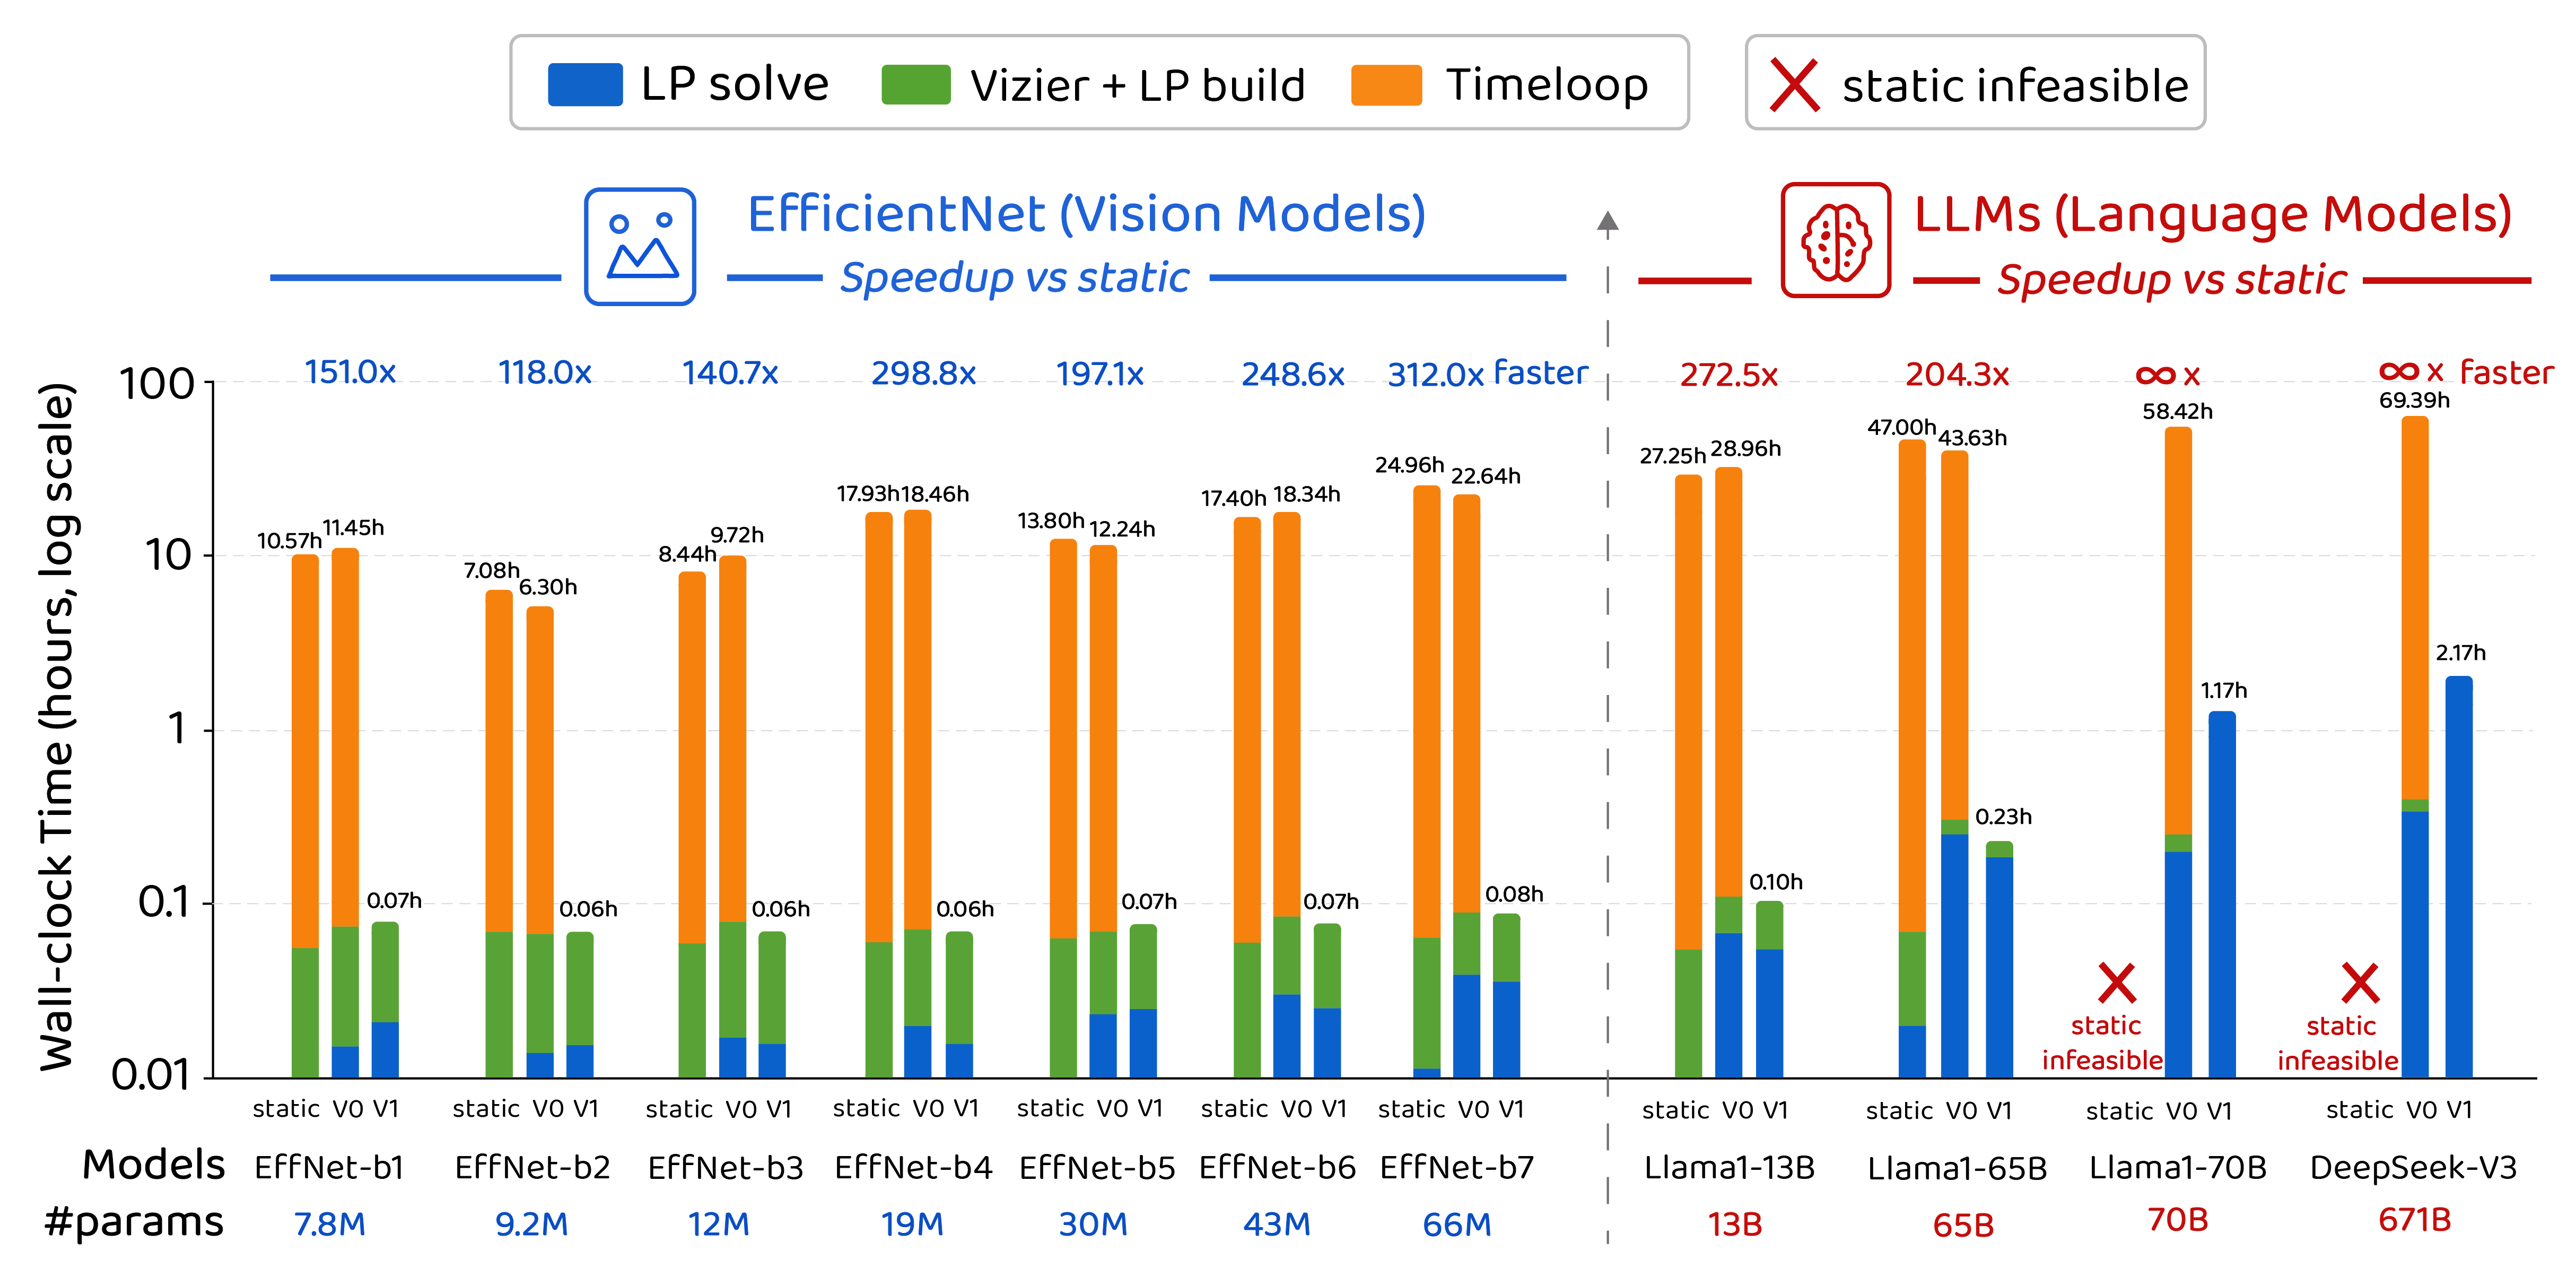
\includegraphics[width=1.0\linewidth]{fig3/wallclock_new_v5.png}
% % % % % \caption{Wall-clock time decomposition and performance acceleration across formulations: CHEETAH-V1's internalized tiling eliminates the Timeloop bottleneck, achieving up to 100–300× faster search than classical static method.}
% % % % % \label{fig:wallclock}
% % % % % \end{figure}

% % % % \begin{figure}[ht!]
% % % %     \centering
% % % % 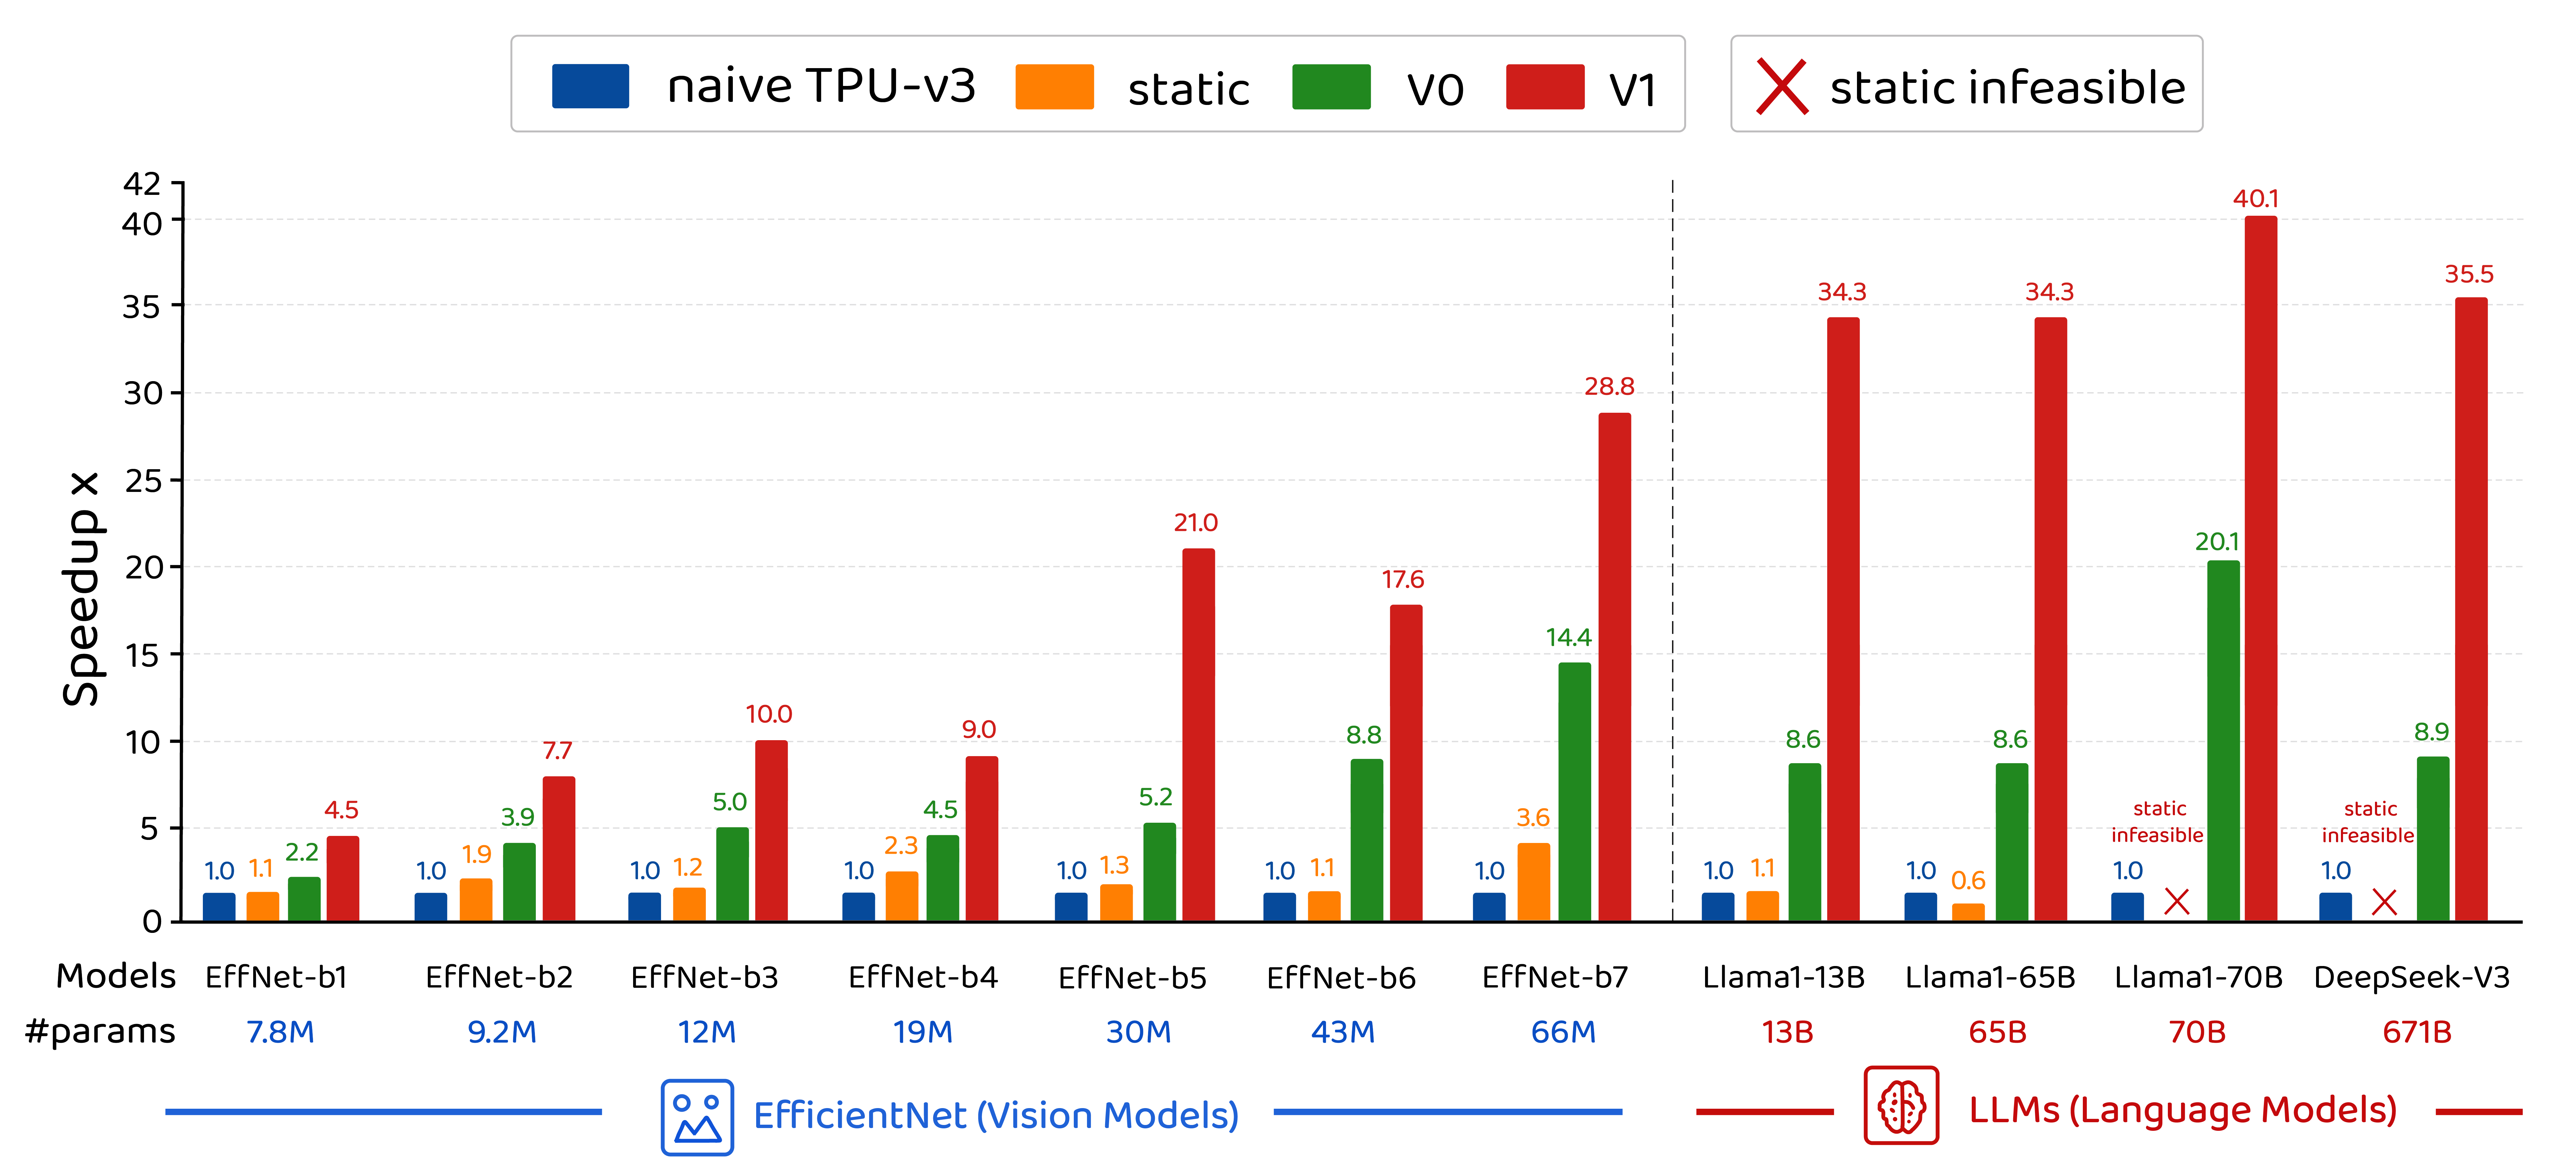
\includegraphics[width=1.0\linewidth]{fig3/speedup_final_v2.png}
% % % % \caption{Speedup over modeled TPU-v3 baseline across formulations and workloads: CHEETAH-V1's joint tiling-fusion optimization achieves up to $\sim$35× acceleration, while static fusion is infeasible on large-scale LLMs.}
% % % % \label{fig:speedup}
% % % % \end{figure}

% % % % % In addition to efficiently enabling more globally optimized accelerator designs, we anticipate that future work may build off this foundation to implement custom Flash Attention type speedup mechanisms for individual hardware (such as RTX5090) and workloads (such as LLama70B) tractably within hours, as well as quickly and efficiently design custom accelerators for targeted inference tasks. 
% % % % % compromise on any single workload; a growing body of evidence suggests that workload-specialized designs can deliver $2$--$6\times$ improvements in performance per watt.
% % % % % The resulting system replaces FAST's sequential Timeloop$\rightarrow$fusion~ILP pipeline with a single LP that jointly optimizes tiling, fusion, and memory scheduling, while preserving Vizier's outer loop over hardware configurations (or replacing it with LLM-guided search).

% % % % % Furthermore, FAST's fusion ILP uses static tensor placement: a tensor is either pinned for the entire inference pass or not at all.
% % % % % This is overly conservative for models with long dependency chains or skip connections, where different tensors are live at different times during execution.
% % % % % A dynamic placement strategy that can evict and re-pin tensors across timesteps could substantially improve global memory utilization. Joint Optimization is the only way to solve the "Memory Wall" for large scale models like DeepSeek-V3.

% % % % % FAST operates via a three-stage sequential pipeline (Figure \ref{fig::workflow}): (1)~a black-box optimizer (Google Vizier \citep{google_vizier}) proposes a hardware configuration defined by 16 hyperparameters---PE grid dimensions, systolic array sizes, buffer capacities, DRAM channels, and batch size; (2)~a scheduling engine (Timeloop \citep{timeloop}) finds the best tiling and mapping for each operation independently given the fixed hardware; and (3)~an integer linear program (ILP) decides which tensors to pin in the on-chip Global Memory to reduce DRAM traffic.
% % % % % The result of each trial---predicted performance per TDP---is fed back to Vizier, which proposes the next hardware configuration, repeating for thousands of trials until convergence.


% % % % % automate the framework with SkyDiscover Loop for profile and context aware co-design. Therefore in less than five hours, we are able to find an more performant design spec than the strongest baseline on designing , in terms of both perf/TDP and speedup. Our experiments also include freezing any hardware at input, and reducing the scheduling, tiling, etc search to just the LP can yield speedups of avg 2.2x than just the base hardware along. We anticipate that future work may build off this foundation to implement custom Flash Attention type speedup mechanisms for individual hardware (such as RTX5090) and workloads (such as LLama70B) tractably within hours. 

% % % % % Our propose the formulation for global co-design for a custom accelerator as a large scale linear program which captures strict dependencies and tradeoffs sequential methods may miss. Our LP formulation captures scheduling, tiling, rematerialization, and is able to solve matrices at scales of $6{,}319 \times 4{,}516$,\ nnz$=829{,}852$ \& $3{,}669{,}793 \times 3{,}263{,}443$,\ nnz$=7{,}342{,}293$ \& $2{,}983{,}450 \times 2{,}504{,}019$,\ nnz$=6{,}094{,}156$ quickly, by utilizing a JAX based large scale solver. Our insight is that despite the challenging large scale of the problem, the structure of the matrices, once formed, retain the same structure. Therefore we are able to design one preconditioning scheme to these large scale systems matrices that can be re-used across any NN. This also allows us to capture dependencies prior methods cannot, for example our formulation introduces a dynamic placement strategy that can evict and re-pin tensors across timesteps could substantially improve global memory utilization. Joint Optimization is the only way to solve the "Memory Wall" for large scale models like DeepSeek-V3. 

% % % % % For EfficientNet-B7 at $L=400$ operations and $T=400$ timesteps, the V1 LP contains approximately $2$ million variables and $5$ million constraints with $15$--$25$ million nonzeros. To better solve such large-scale LP problems more efficiently, we implement our own variant of a GPU-accelerated solver based on recent primal-dual LP algorithm \citep{applegate2022practicallargescalelinearprogramming}. We extend its original formulation in various ways and benchmark our implementation compared to existing commercial SciPy solvers, which showcase the advantage of our solver. To keep the main context clean and focused, we defer LP solver-related details to Appendix \ref{app:solver}.

% % % % % A large number of black box optimization tools to handle this large search space have been recently proposed, such as Google's Vizier, Meta's AX, and Optuna. In addition search strategies are also explored, for example Google's Vizier proposes numerous methods Gaussian Process Upper Confidence Bound, Eagle Strategy as a metaheuristic optimization algorithm designed for global optimization via a two-stage hybrid approach that combines global exploration with intensive local search, and Linear Combination Swarm (LCS). However these methods share certain limitations, since they cannot globally capture the tradeoffs and tensions between sequential decisions and rely on brute force iterations. This requires human engineers to spend months of compute and thousands of repetitive trials to get improvements, without feedback on what might be globally optimal. 

% % % % % While this sequential decomposition makes the problem tractable, it introduces a fundamental limitation: \emph{each stage takes the previous stage's output as fixed input, preventing the discovery of solutions that require trading off across stages.} Consider a concrete example: for a depthwise-separable convolution layer in a NN, a search tool such as Timeloop might select a tiling configuration that maximizes compute utilization at $74\%$, producing an activation working set of $6$ MiB. THe stacked The downstream fusion ILP solver tool receives this fixed working set size, cannot fit the tensor into the $128$ MiB Global Memory alongside other pinned tensors. However, an alternative tiling configuration with slightly lower utilization ($70\%$) might produce a working set of only $3$ MiB, enabling the fusion solver to pin an additional weight tensor that eliminates a DRAM bottleneck entirely, thus yielding a net $>20\%$ cycle reduction despite the $4\%$ utilization loss. Therefore these sequential pipelines systematically misses such cross-stage trade-offs.

% % % % % The rapid evolution of deep learning workloads has created a compelling opportunity for domain-optimized inference accelerators.
% % % % % Production models now serve billions of daily users, and the computational demands of architectures based on depthwise-separable convolutions (EfficientNet), self-attention (BERT, LLaMA), mixture-of-experts (DeepSeek-V3, Mixtral), and state-space models (Mamba) differ dramatically in their compute-to-memory ratios, tensor shapes, and data reuse patterns. However although the NN training strategy has been scaled up and we've done a lot of work on it, we now face the inference bottle neck era since general-purpose hardware, Nvidia's gaming GPUs are not necessarily optimized for deep learning tasks, and leaves a huge amount of compute on the table.


% % % % page edit

% % % \section{Introduction}
% % % \label{sec:introduction}

% % % \begin{figure}[ht!]
% % %     \centering
% % %     \includegraphics[width=1.0\linewidth]{figs/cheetah_v4.png}
% % %     % \caption{\textbf{FAST vs.\ FAST-CORGI pipeline comparison.} 
% % % \caption{Sequential vs Our Unified Optimization Paradigm.
% % % (Left) Baseline methods decouple hardware search, operation-level tiling, and static fusion; precluding cross-stage trade-offs.
% % % (Right) CHEETAH presents a unified LLM-driven LP-solver-based framework that jointly optimizes tiling, placement, and rematerialization while learning from a causal ledger.}
% % % \label{fig::workflow}
% % % \end{figure}
% % % % The rapid evolution of deep learning workloads varies from convolutions to self-attention (LLaMA), mixture-of-experts (DeepSeek-V3), and state-space models (Mamba). These diverse architectures serve billions of daily users, and have fundamentally shifted the requirements for hardware acceleration. As foundation models continue to scale in parameters, the primary cost and bottleneck of model deployment has shifted from training to inference. Therefore much recent research has been focused on optimizing for more efficient execution and throughput across diverse, high-dimensional workloads. General-purpose GPUs remain largely designed for graphics-heavy throughput, and leave substantial efficiency and compute on the table at these tasks. Therefore we are motivated to design targeted accelerators that are optimized for handling the varying tensor shapes and data-reuse patterns of modern deep learning architectures.
% % % % Much research has been done in accelerating inference through custom accelerator design, more efficient neural network (NN) batching algorithms, and domain specific packages and languages that aim to speed up general NN inference. For example, the widely adopted Flash Attention uses tiling to provide significant speedups by optimizing memory movement between SRAM and DRAM. Co-design takes this a step further by aiming to optimize hardware, software and scheduling to unlock performance neither could reach independently. The traditional framework of doing this is a sequential pipeline of heuristics tools, requiring human engineers to iterate through a large search space for months from testing for the size of DRAM, to determining higher level scheduling problems. Optimizing each piece of this complex pipeline is extremely challenging, since hardware datapaths, software schedules, and compiler transforms across a combinatorial space exceeding $\mathcal O(10^{2300})$.
% % % The AI inference demand is expected to grow by $10,000\times$ over the next 5 years \citep{cra2026aifuture}. General-purpose accelerators leave significant efficiency gains unrealized, which motivates the design of targeted custom accelerators. Co-design, which jointly optimizes hardware-software (HW/SW), and scheduling for target workloads, offers a path to unlock performance efficiency for the upcoming inference era. However, the prevailing approach relies on sequential pipelines of heuristic tools, a slow, human-driven process navigating a combinatorial search space exceeding $O(10^{2300})$ \citep{zhang_fast}. State-of-the-art frameworks like FAST \citep{zhang_fast} improve on through an automated flow (a hardware proposer feeds an operation-level tiling agent, which feeds a downstream fusion solver), but remain fundamentally decoupled.  For example, a tiling configuration that is \textit{locally} optimal for one layer may create an activation footprint that later prevents \textit{global} fusion, while a slightly slower tiling might shrink the working set enough to eliminate a DRAM bottleneck entirely. Sequential pipelines are systematically unable to express these interactions, leading to locally good but globally sub-optimal designs.

% % % % The co-design problem is increasingly important as inference efficiency is the dominant AI workload and is rapidly growing. Therefore industry leaders such as NVIDIA and Google have designed chips for improved hardware-native agentic AI and , and state-of-the-art frameworks such as FAST, address this through a sequential decomposition of heuristics (a hardware proposer feeds an operation-level tiling agent, which feeds a downstream fusion solver). While FAST-generated accelerators can provide increased speedups over baseline TPU-v3, this decoupled approach is limited since it cannot capture cross-stage trade-offs. A tiling configuration that is \textit{locally} optimal for one layer may create an activation footprint that later prevents \textit{global} fusion, while a slightly slower tiling might shrink the working set enough to eliminate a DRAM bottleneck entirely. Sequential pipelines are systematically unable to express these interactions, leading to locally good but globally sub-optimal designs. 
% % % We prove that by unifying the design space into a single convex relaxation, we find global optima that were previously  infeasible. Specifically, we introduce CHEETAH: a custom inference accelerator design framework that unlocks globally optimized designs with a dual-loop. Our inner-loop is a novel large-scale Linear Program (LP) to precisely mathematically model strict design decisions and constraints that must not be violated. The LP captures trade-offs for targeted workloads through time-indexed placement and rematerialization, thus allowing tensors to be dynamically pinned, evicted, recomputed across inference timesteps. We further extend our reformulation to internalize tiling selection into the LP, by introducing Pareto-pruned tiling variables and the McCormick linearization (a convex relaxation used for optimization of bilinear problems \citep{mccormick1976computability}). By exploiting the structural invariance of our matrices across hardware trials, we also adapt a GPU-accelerated primal-dual solver in JAX \citep{jax2018github} that can resolve millions of variables to rapidly reduce trial time from days to hours. This allows the LP solver to jointly reason about hardware configuration, activation placement, and weight pinning in a single pass, while providing feedback signal via Lagrangian duals.

% % % Our outer-loop framework stacks a black-box optimizer (Google Vizier \citep{google_vizier}) to propose candidate hardware configurations defined by a set of hyperparameters (e.g., processing element grid dimensions, systolic array sizes, DRAM size, etc), while a LLM is used for efficient search-space steering. The LLM acts as a causal architect, interpreting a compact trial ledger of roofline checks and LP feedback diagnostics to propose constrained architectural search input for Vizier. This prevents the search-space gaming typical of black-box optimizers in wide design regions, and reduces the need for thousands of sequential trials via Bayesian search strategies in Vizier to learn good vs bad neighborhoods in search topology. Our results demonstrate that the LLM Architect framework further reduces invalid hardware trials from 24.5\% under vanilla Vizier to 5.9\%, while reaching the Pareto frontier 4.5x faster than the next strongest baseline. We validate all results with Model Flop Utilization (MFU) and roofline lower-bound audits, ensuring predicted latencies are physically grounded in compute and memory throughput limits. 
% % % % \todo{Add best of both worlds, strengths from principled LP side, from LLM aggregate info side}
% % % % \todo{Aggregates past experience to gain insight into steering hardware-software co-design. We offload the strict solves, with constraints that must the strictly respected, to the LP solve part. This combines the best of both worlds.} 
% % % \paragraph{Contributions.} We reformulated the fundamental HW/SW co-design problem into a unified  framework in CHEETAH, combining principled mathematical rigor of the LP formulation to solve strict design decisions optimally, with the powerful aggregation and causal learning of an LLM Architect outer loop for meta-optimization. Our open-source repository for full reproducibility is at \href{https://anonymous.4open.science/r/CHEETAH-B268/readme}{https://anonymous.4open.science/r/CHEETAH-B268/}.

% % % \begin{enumerate}
% % %     \item \textbf{CHEETAH-V0 - Dynamic Placement with Rematerialization:}
% % %     We introduce time-indexed LP variables $p_{i,t}^k$ and rematerialization variables $r_{i,t}$ to enable cheap recompute operations (\eg, depthwise convolutions that account for only $5\%$ of FLOPs but produce large activations) instead of paying DRAM reload costs, supporting skip connections and multi-fanout nodes.

% % %     \item \textbf{CHEETAH-V1 - Joint Tiling-Fusion:}
% % %     We unify tiling and fusion into a single LP problem by introducing tiling selection variables $y_{i,c}$, and employ McCormick envelopes to exactly linearize the bilinear interaction between tiling and tensor pinning. This technique yields a tight, parameter-free LP relaxation, and the coupling internalizes the tiling-placement trade-off to discover optimal design points that sequential pipelines systematically miss.
% % %     % This enables the LP to discover trade-offs where accepting a suboptimal tiling configuration enables superior fusion, or vice versa---precisely the cross-stage interactions that the sequential pipeline cannot capture.
% % %     \item \textbf{LLM-guided Causal Architect:} The LLM outer loop steers hardware search by interpreting Lagrangian sensitivity signals and a Causal Ledger of past trials to perform targeted subspace interventions, transforming black-box search into a structured, diagnostic-driven process. The Architect guides Vizier through widened search spaces, reducing invalid trials by ${\sim}4\times$ while preserving the global optimal score, and enables profile-specific designs (speech models may emphasize latency, while data synthesis models may prioritize bandwidth). 
% % %     \item \textbf{Speedup:} Our method demonstrates an average speedup of $\sim22.07\times$ over the baseline across a wide range of $11$ vision and language models. 

% % %     % profiles into consideration to push the black-box optimizer responsible for hardware suggestions to output with structured reasoning about architectural trade-offs. 

% % % \end{enumerate}

% % % \begin{figure}[ht!]
% % %     \centering
% % % 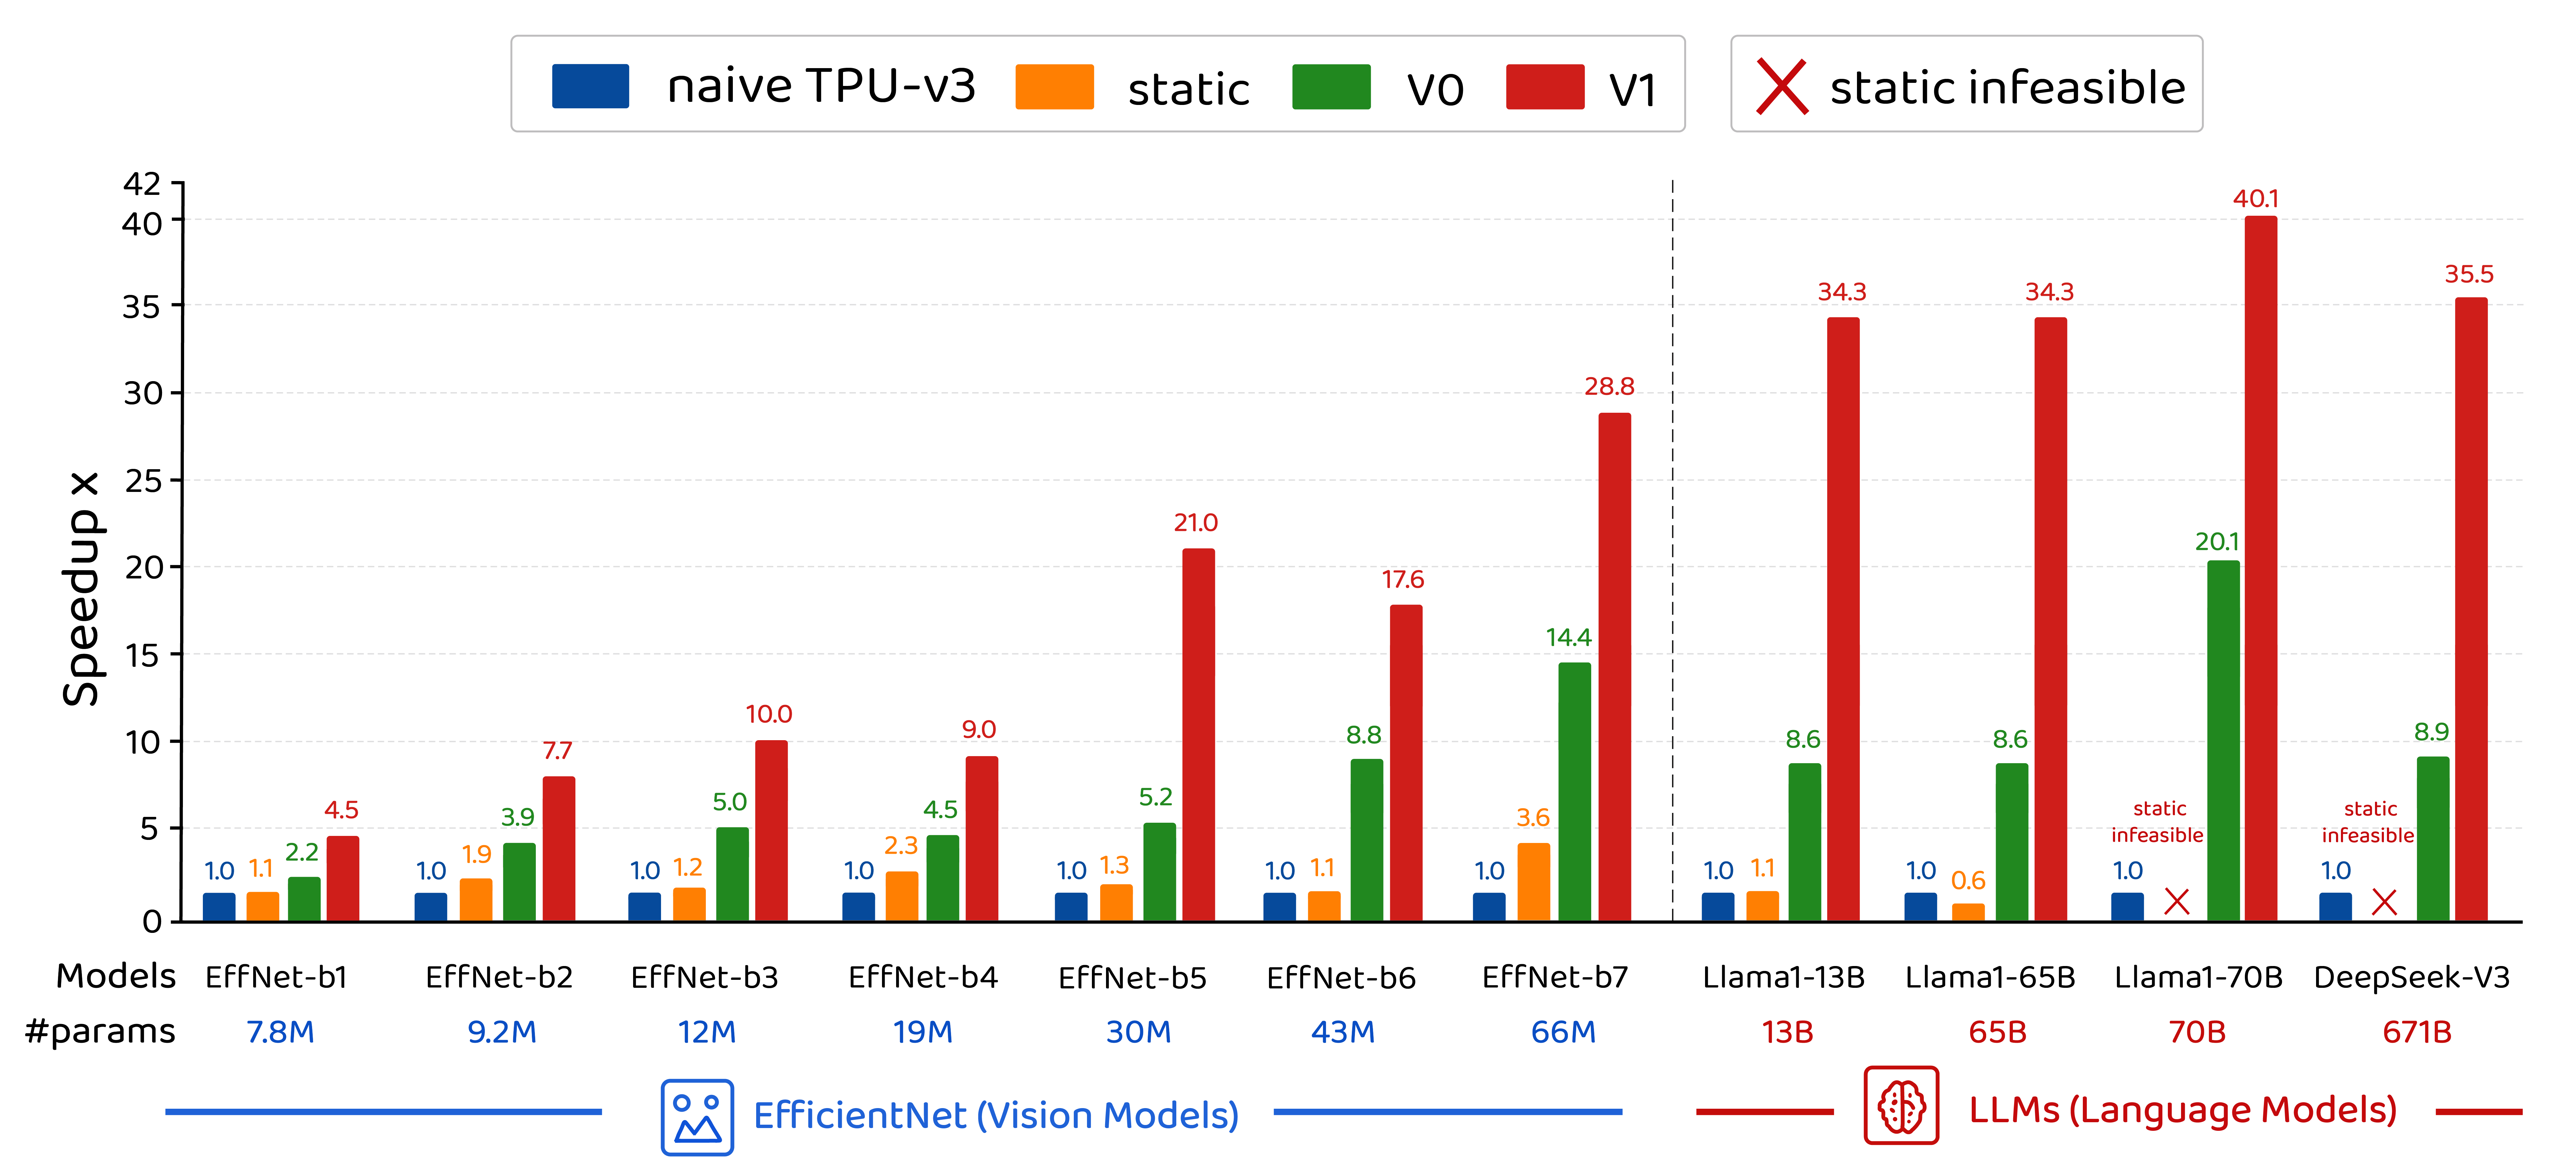
\includegraphics[width=1.0\linewidth]{fig3/speedup_final_v2.png}
% % % \caption{Speedup over modeled TPU-v3 baseline across formulations and workloads: CHEETAH-V1's joint tiling-fusion optimization achieves up to $\sim$40.1$\times$ acceleration, while static fusion is infeasible on large-scale LLMs. Progressive gains are visible across formulations: V0's dynamic placement improves over static by $2$--$20\times$, while V1's joint tiling-fusion adds another $2$--$4\times$ on top. See Section~\ref{sec:experiments} for full analysis and wall-clock time breakdowns.}
% % % \label{fig:speedup}
% % % \end{figure}

% % % % In addition to efficiently enabling more globally optimized accelerator designs, we anticipate that future work may build off this foundation to implement custom Flash Attention type speedup mechanisms for individual hardware (such as RTX5090) and workloads (such as LLama70B) tractably within hours, as well as quickly and efficiently design custom accelerators for targeted inference tasks. 
% % % % compromise on any single workload; a growing body of evidence suggests that workload-specialized designs can deliver $2$--$6\times$ improvements in performance per watt.
% % % % The resulting system replaces FAST's sequential Timeloop$\rightarrow$fusion~ILP pipeline with a single LP that jointly optimizes tiling, fusion, and memory scheduling, while preserving Vizier's outer loop over hardware configurations (or replacing it with LLM-guided search).

% % % % Furthermore, FAST's fusion ILP uses static tensor placement: a tensor is either pinned for the entire inference pass or not at all.
% % % % This is overly conservative for models with long dependency chains or skip connections, where different tensors are live at different times during execution.
% % % % A dynamic placement strategy that can evict and re-pin tensors across timesteps could substantially improve global memory utilization. Joint Optimization is the only way to solve the "Memory Wall" for large scale models like DeepSeek-V3.

% % % % FAST operates via a three-stage sequential pipeline (Figure \ref{fig::workflow}): (1)~a black-box optimizer (Google Vizier \citep{google_vizier}) proposes a hardware configuration defined by 16 hyperparameters---PE grid dimensions, systolic array sizes, buffer capacities, DRAM channels, and batch size; (2)~a scheduling engine (Timeloop \citep{timeloop}) finds the best tiling and mapping for each operation independently given the fixed hardware; and (3)~an integer linear program (ILP) decides which tensors to pin in the on-chip Global Memory to reduce DRAM traffic.
% % % % The result of each trial---predicted performance per TDP---is fed back to Vizier, which proposes the next hardware configuration, repeating for thousands of trials until convergence.


% % % % automate the framework with SkyDiscover Loop for profile and context aware co-design. Therefore in less than five hours, we are able to find an more performant design spec than the strongest baseline on designing , in terms of both perf/TDP and speedup. Our experiments also include freezing any hardware at input, and reducing the scheduling, tiling, etc search to just the LP can yield speedups of avg 2.2x than just the base hardware along. We anticipate that future work may build off this foundation to implement custom Flash Attention type speedup mechanisms for individual hardware (such as RTX5090) and workloads (such as LLama70B) tractably within hours. 

% % % % Our propose the formulation for global co-design for a custom accelerator as a large scale linear program which captures strict dependencies and tradeoffs sequential methods may miss. Our LP formulation captures scheduling, tiling, rematerialization, and is able to solve matrices at scales of $6{,}319 \times 4{,}516$,\ nnz$=829{,}852$ \& $3{,}669{,}793 \times 3{,}263{,}443$,\ nnz$=7{,}342{,}293$ \& $2{,}983{,}450 \times 2{,}504{,}019$,\ nnz$=6{,}094{,}156$ quickly, by utilizing a JAX based large scale solver. Our insight is that despite the challenging large scale of the problem, the structure of the matrices, once formed, retain the same structure. Therefore we are able to design one preconditioning scheme to these large scale systems matrices that can be re-used across any NN. This also allows us to capture dependencies prior methods cannot, for example our formulation introduces a dynamic placement strategy that can evict and re-pin tensors across timesteps could substantially improve global memory utilization. Joint Optimization is the only way to solve the "Memory Wall" for large scale models like DeepSeek-V3. 

% % % % For EfficientNet-B7 at $L=400$ operations and $T=400$ timesteps, the V1 LP contains approximately $2$ million variables and $5$ million constraints with $15$--$25$ million nonzeros. To better solve such large-scale LP problems more efficiently, we implement our own variant of a GPU-accelerated solver based on recent primal-dual LP algorithm \citep{applegate2022practicallargescalelinearprogramming}. We extend its original formulation in various ways and benchmark our implementation compared to existing commercial SciPy solvers, which showcase the advantage of our solver. To keep the main context clean and focused, we defer LP solver-related details to Appendix \ref{app:solver}.

% % % % A large number of black box optimization tools to handle this large search space have been recently proposed, such as Google's Vizier, Meta's AX, and Optuna. In addition search strategies are also explored, for example Google's Vizier proposes numerous methods Gaussian Process Upper Confidence Bound, Eagle Strategy as a metaheuristic optimization algorithm designed for global optimization via a two-stage hybrid approach that combines global exploration with intensive local search, and Linear Combination Swarm (LCS). However these methods share certain limitations, since they cannot globally capture the tradeoffs and tensions between sequential decisions and rely on brute force iterations. This requires human engineers to spend months of compute and thousands of repetitive trials to get improvements, without feedback on what might be globally optimal. 

% % % % While this sequential decomposition makes the problem tractable, it introduces a fundamental limitation: \emph{each stage takes the previous stage's output as fixed input, preventing the discovery of solutions that require trading off across stages.} Consider a concrete example: for a depthwise-separable convolution layer in a NN, a search tool such as Timeloop might select a tiling configuration that maximizes compute utilization at $74\%$, producing an activation working set of $6$ MiB. THe stacked The downstream fusion ILP solver tool receives this fixed working set size, cannot fit the tensor into the $128$ MiB Global Memory alongside other pinned tensors. However, an alternative tiling configuration with slightly lower utilization ($70\%$) might produce a working set of only $3$ MiB, enabling the fusion solver to pin an additional weight tensor that eliminates a DRAM bottleneck entirely, thus yielding a net $>20\%$ cycle reduction despite the $4\%$ utilization loss. Therefore these sequential pipelines systematically misses such cross-stage trade-offs.

% % % % The rapid evolution of deep learning workloads has created a compelling opportunity for domain-optimized inference accelerators.
% % % % Production models now serve billions of daily users, and the computational demands of architectures based on depthwise-separable convolutions (EfficientNet), self-attention (BERT, LLaMA), mixture-of-experts (DeepSeek-V3, Mixtral), and state-space models (Mamba) differ dramatically in their compute-to-memory ratios, tensor shapes, and data reuse patterns. However although the NN training strategy has been scaled up and we've done a lot of work on it, we now face the inference bottle neck era since general-purpose hardware, Nvidia's gaming GPUs are not necessarily optimized for deep learning tasks, and leaves a huge amount of compute on the table.


% % % page limit edit

% % % \section{Introduction}
% % % \label{sec:introduction}

% % % \begin{figure}[ht!]
% % %     \centering
% % %     \includegraphics[width=1.0\linewidth]{figs/cheetah_v4.png}
% % % \caption{Sequential vs Unified Optimization Paradigm Comparison.
% % % (Left) Baseline methods decouple hardware search, operation-level tiling, and static fusion; precluding cross-stage trade-offs.
% % % (Right) CHEETAH presents a unified LLM-driven LP-solver-based framework that jointly optimizes tiling, placement, and rematerialization while learning from a causal ledger.}
% % % \label{fig::workflow}
% % % \end{figure}
% % % % The rapid evolution of deep learning workloads varies from convolutions to self-attention (LLaMA), mixture-of-experts (DeepSeek-V3), and state-space models (Mamba). These diverse architectures serve billions of daily users, and have fundamentally shifted the requirements for hardware acceleration. As foundation models continue to scale in parameters, the primary cost and bottleneck of model deployment has shifted from training to inference. Therefore much recent research has been focused on optimizing for more efficient execution and throughput across diverse, high-dimensional workloads. General-purpose GPUs remain largely designed for graphics-heavy throughput, and leave substantial efficiency and compute on the table at these tasks. Therefore we are motivated to design targeted accelerators that are optimized for handling the varying tensor shapes and data-reuse patterns of modern deep learning architectures.
% % % % Much research has been done in accelerating inference through custom accelerator design, more efficient neural network (NN) batching algorithms, and domain specific packages and languages that aim to speed up general NN inference. For example, the widely adopted Flash Attention uses tiling to provide significant speedups by optimizing memory movement between SRAM and DRAM. Co-design takes this a step further by aiming to optimize hardware, software and scheduling to unlock performance neither could reach independently. The traditional framework of doing this is a sequential pipeline of heuristics tools, requiring human engineers to iterate through a large search space for months from testing for the size of DRAM, to determining higher level scheduling problems. Optimizing each piece of this complex pipeline is extremely challenging, since hardware datapaths, software schedules, and compiler transforms across a combinatorial space exceeding $\mathcal O(10^{2300})$.
% % % The AI inference demand is expected to grow by $10,000\times$ over the next 5 years \citep{cra2026aifuture}. General-purpose accelerators leave significant efficiency gains unrealized, which motivates the design of targeted custom accelerators. Co-design, which jointly optimizes hardware, software, and scheduling for target workloads, offers a path to unlock performance efficiency for the upcoming inference era. However, the prevailing approach relies on sequential pipelines of heuristic tools, a slow, human-driven process navigating a combinatorial search space exceeding $O(10^{2300})$ \citep{zhang_fast}. State-of-the-art frameworks like FAST \citep{zhang_fast} improve on through an automated flow (a hardware proposer feeds an operation-level tiling agent, which feeds a downstream fusion solver), but remain fundamentally decoupled.  For example, a tiling configuration that is \textit{locally} optimal for one layer may create an activation footprint that later prevents \textit{global} fusion, while a slightly slower tiling might shrink the working set enough to eliminate a DRAM bottleneck entirely. Sequential pipelines are systematically unable to express these interactions, leading to locally good but globally sub-optimal designs.

% % % % The co-design problem is increasingly important as inference efficiency is the dominant AI workload and is rapidly growing. Therefore industry leaders such as NVIDIA and Google have designed chips for improved hardware-native agentic AI and , and state-of-the-art frameworks such as FAST, address this through a sequential decomposition of heuristics (a hardware proposer feeds an operation-level tiling agent, which feeds a downstream fusion solver). While FAST-generated accelerators can provide increased speedups over baseline TPU-v3, this decoupled approach is limited since it cannot capture cross-stage trade-offs. A tiling configuration that is \textit{locally} optimal for one layer may create an activation footprint that later prevents \textit{global} fusion, while a slightly slower tiling might shrink the working set enough to eliminate a DRAM bottleneck entirely. Sequential pipelines are systematically unable to express these interactions, leading to locally good but globally sub-optimal designs. 
% % % We prove that by unifying the design space into a single convex relaxation, we find global optima that were previously  infeasible. Specifically, we introduce CHEETAH: a custom inference accelerator design framework that unlocks globally optimized designs with a dual-loop engine (See Figure \ref{fig::workflow}). Our inner-loop is a novel large-scale Linear Program (LP) to precisely mathematically model strict design decisions and constraints that must not be violated. The LP captures trade-offs for targeted workloads through time-indexed placement and rematerialization, thus allowing tensors to be dynamically pinned, evicted, recomputed across inference timesteps. We further extend our reformulation to internalize tiling selection into the LP, by introducing Pareto-pruned tiling variables and the McCormick linearization (a convex relaxation used for optimization of bilinear problems \citep{mccormick1976computability}). By exploiting the structural invariance of our matrices across hardware trials, we also adapt a GPU-accelerated primal-dual solver in JAX that can resolve millions of variables to rapidly reduce trial time from days to hours. This allows the LP solver to jointly reason about hardware configuration, activation placement, and weight pinning in a single pass, while providing feedback signal via Lagrangian duals.

% % % Our outer-loop framework stacks a black-box optimizer (Google Vizier \citep{google_vizier}) to propose candidate hardware configurations defined by a set of hyperparameters (e.g., processing element grid dimensions, systolic array sizes, DRAM size, etc), while a LLM is used for efficient search-space steering. The LLM acts as a causal architect, interpreting a compact trial ledger of roofline checks and LP feedback diagnostics to propose constrained architectural search input for Vizier. This prevents the search-space gaming typical of black-box optimizers in wide design regions, and reduces the need for thousands of sequential trails via Bayesian search strategies in Vizier to learn good vs bad neighborhoods in search topology. Our results demonstrate that the LLM-Architect framework further reduces invalid hardware trials from 24.5\% under vanilla Vizier to 5.9\%, while reaching the Pareto frontier 4.5x faster than the next strongest baseline. We validate all results with Model Flop Utilization (MFU)  and roofline lower-bound audits, ensuring predicted latencies are physically grounded in compute and memory throughput limits. 
% % % % \todo{Add best of both worlds, strengths from principled LP side, from LLM aggregate info side}
% % % % \todo{Aggregates past experience to gain insight into steering hardware-software co-design. We offload the strict solves, with constraints that must the strictly respected, to the LP solve part. This combines the best of both worlds.} 
% % % \paragraph{Contributions.} We reformulated the fundamental HW/SW co-design problem into a unified  framework in CHEETAH, combining principled mathematical rigor of the LP formulation to solve strict design decisions optimally, with the powerful aggregation and causal learning of an LLM Architect outer loop for meta-optimization. Our open-source repository for full reproducibility is at \href{https://anonymous.4open.science/r/CHEETAH-B268/readme}{https://anonymous.4open.science/r/CHEETAH-B268/}.

% % % \begin{enumerate}
% % %     \item \textbf{CHEETAH-V0 - Dynamic Placement with Rematerialization:}
% % %     We introduce the time-indexed and rematerialization variables to enable cheap recompute operations (\eg, depthwise convolutions that account for only $5\%$ of FLOPs but produce large activations) instead of paying DRAM reload costs. This addresses the restrictions of existing baseline methods where activations can only be pinned between consecutively-executed operations, and supports skip connections and multi-fanout nodes.

% % %     \item \textbf{CHEETAH-V1 - Joint Tiling-Fusion:}
% % %     We unify tiling and fusion into a single LP problem by introducing tiling selection variables $y_{i,c}$, and employ McCormick envelopes to exactly linearize the bilinear interaction between tiling and tensor pinning. This technique yields a tight, parameter-free LP relaxation, and the coupling internalizes the tiling-placement trade-off to discover optimal design points that sequential pipelines systematically miss.
% % %     % This enables the LP to discover trade-offs where accepting a suboptimal tiling configuration enables superior fusion, or vice versa---precisely the cross-stage interactions that the sequential pipeline cannot capture.
% % %     \item \textbf{LLM-guided Causal Architect:} The LLM outer loop steers hardware search and bridges high-level architectural reasoning with low-level solver duals. It interprets Lagrangian sensitivity signals to perform targeted subspace interventions, transforming black-box search into a structured, diagnostic-driven process. We use a context-aware LLM Architect to propose good search areas as input to Vizier (a black-box Bayesian optimizer). Feedback signals are aggregated across historical trials through both the Causal Ledger and the LP solver. The Architect then guides Vizier through widened search spaces, reducing invalid trials by ${\sim}4\times$ while preserving the global optimal score, while enabling profile-specific designs (speech models may emphasize latency, while data synthesis models may prioritize bandwidth). 
% % %     \item \textbf{Speedup:} We show that across a large suite of vision and language modeling workloads, CHEETAH results in an average of 20.9X faster designs than prior work. 

% % %     % profiles into consideration to push the black-box optimizer responsible for hardware suggestions to output with structured reasoning about architectural trade-offs. 

% % % \end{enumerate}

% % % We anticipate that future work may build from this framework in two ways: as an end-to-end co-design system for efficient accelerators, and as an automated optimization engine for existing hardware. By fixing the architecture, the inner loop derives optimal tiling and scheduling strategies that can act as custom speedups for targeted inference tasks.

% % % % \begin{figure}[ht!] 
% % % %     \centering
% % % % 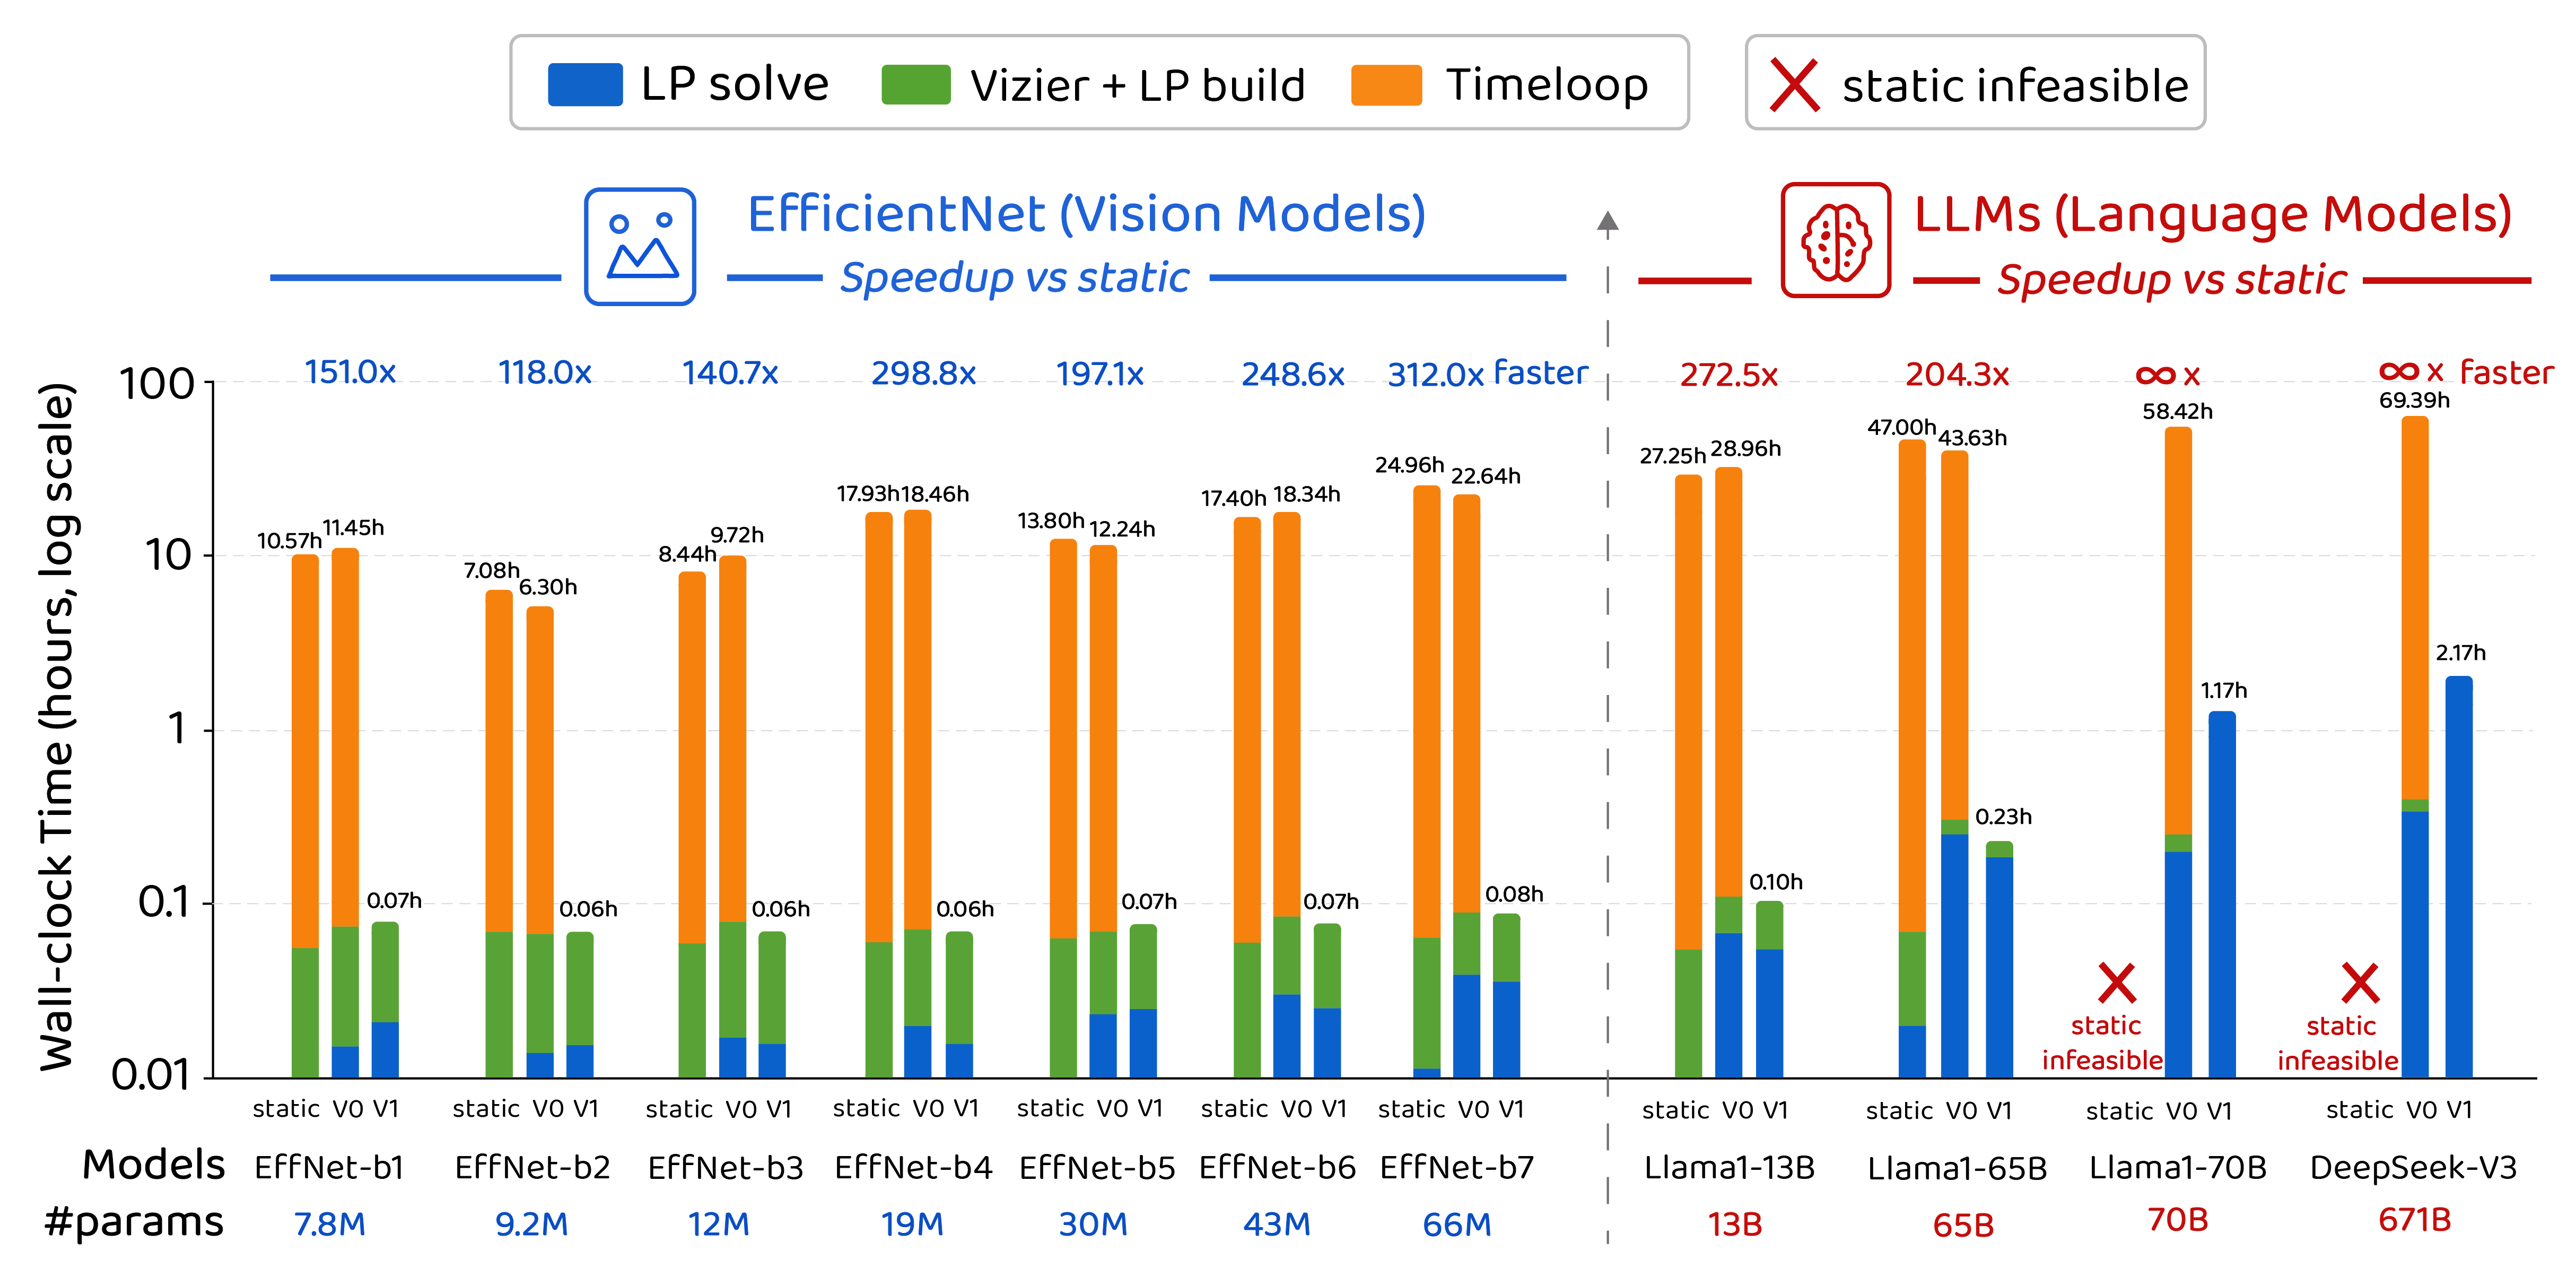
\includegraphics[width=1.0\linewidth]{fig3/wallclock_new_v5.png}
% % % % \caption{Wall-clock time decomposition and performance acceleration across formulations: CHEETAH-V1's internalized tiling eliminates the Timeloop bottleneck, achieving up to 100–300× faster search than classical static method.}
% % % % \label{fig:wallclock}
% % % % \end{figure}

% % % \begin{figure}[ht!]
% % %     \centering
% % % 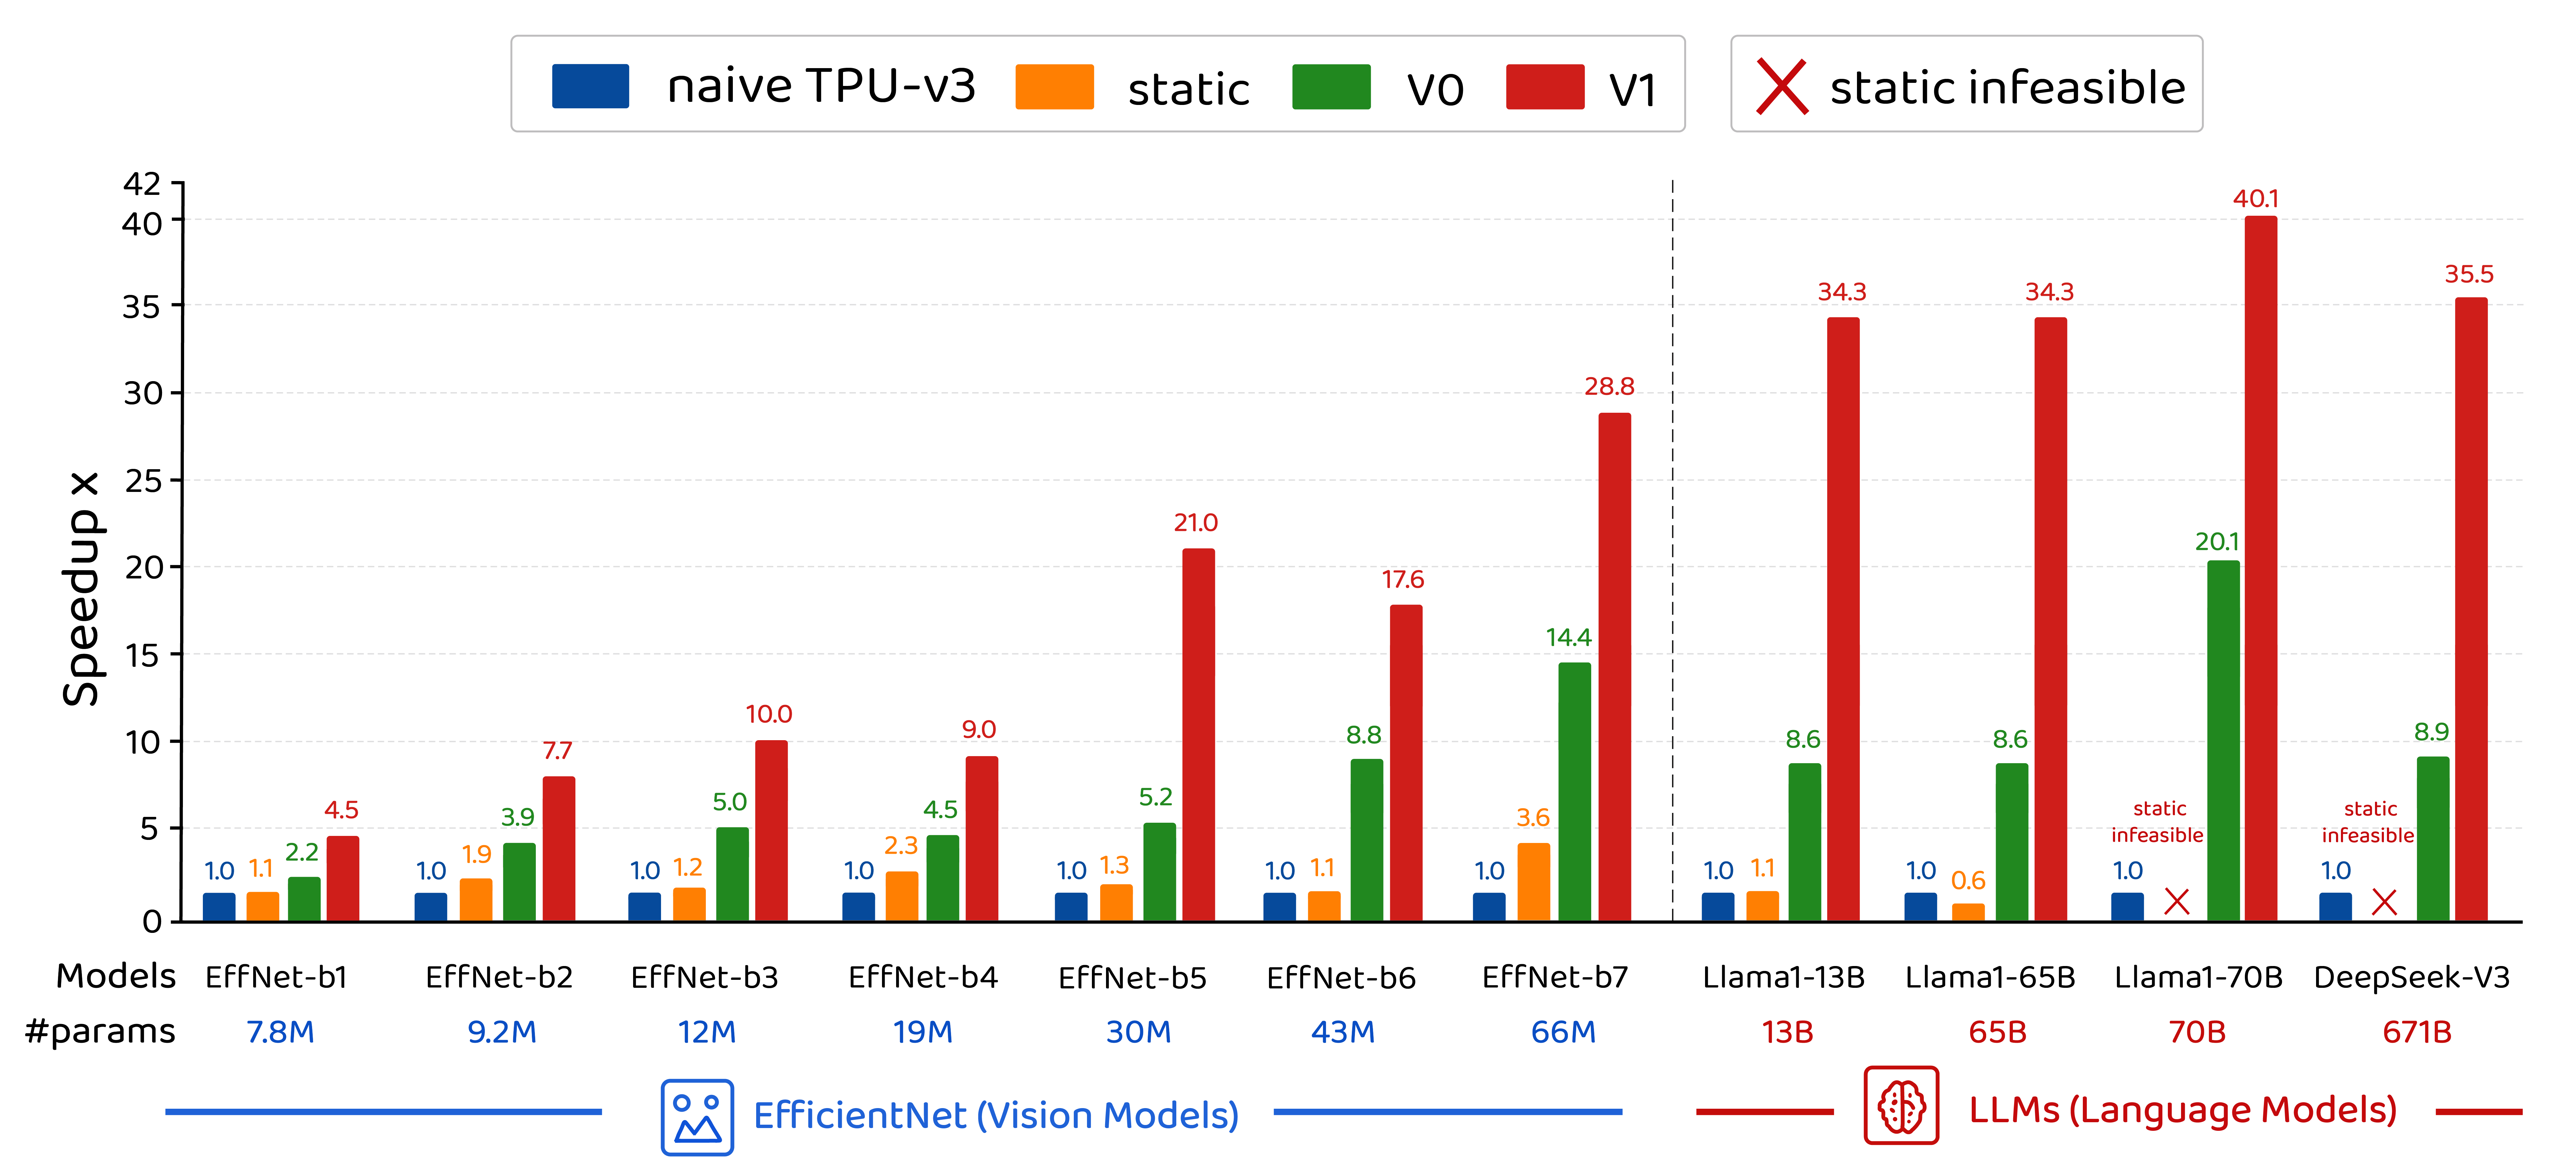
\includegraphics[width=1.0\linewidth]{fig3/speedup_final_v2.png}
% % % \caption{Speedup over modeled TPU-v3 baseline across formulations and workloads: CHEETAH-V1's joint tiling-fusion optimization achieves up to $\sim$35× acceleration, while static fusion is infeasible on large-scale LLMs.}
% % % \label{fig:speedup}
% % % \end{figure}

% % % % In addition to efficiently enabling more globally optimized accelerator designs, we anticipate that future work may build off this foundation to implement custom Flash Attention type speedup mechanisms for individual hardware (such as RTX5090) and workloads (such as LLama70B) tractably within hours, as well as quickly and efficiently design custom accelerators for targeted inference tasks. 
% % % % compromise on any single workload; a growing body of evidence suggests that workload-specialized designs can deliver $2$--$6\times$ improvements in performance per watt.
% % % % The resulting system replaces FAST's sequential Timeloop$\rightarrow$fusion~ILP pipeline with a single LP that jointly optimizes tiling, fusion, and memory scheduling, while preserving Vizier's outer loop over hardware configurations (or replacing it with LLM-guided search).

% % % % Furthermore, FAST's fusion ILP uses static tensor placement: a tensor is either pinned for the entire inference pass or not at all.
% % % % This is overly conservative for models with long dependency chains or skip connections, where different tensors are live at different times during execution.
% % % % A dynamic placement strategy that can evict and re-pin tensors across timesteps could substantially improve global memory utilization. Joint Optimization is the only way to solve the "Memory Wall" for large scale models like DeepSeek-V3.

% % % % FAST operates via a three-stage sequential pipeline (Figure \ref{fig::workflow}): (1)~a black-box optimizer (Google Vizier \citep{google_vizier}) proposes a hardware configuration defined by 16 hyperparameters---PE grid dimensions, systolic array sizes, buffer capacities, DRAM channels, and batch size; (2)~a scheduling engine (Timeloop \citep{timeloop}) finds the best tiling and mapping for each operation independently given the fixed hardware; and (3)~an integer linear program (ILP) decides which tensors to pin in the on-chip Global Memory to reduce DRAM traffic.
% % % % The result of each trial---predicted performance per TDP---is fed back to Vizier, which proposes the next hardware configuration, repeating for thousands of trials until convergence.


% % % % automate the framework with SkyDiscover Loop for profile and context aware co-design. Therefore in less than five hours, we are able to find an more performant design spec than the strongest baseline on designing , in terms of both perf/TDP and speedup. Our experiments also include freezing any hardware at input, and reducing the scheduling, tiling, etc search to just the LP can yield speedups of avg 2.2x than just the base hardware along. We anticipate that future work may build off this foundation to implement custom Flash Attention type speedup mechanisms for individual hardware (such as RTX5090) and workloads (such as LLama70B) tractably within hours. 

% % % % Our propose the formulation for global co-design for a custom accelerator as a large scale linear program which captures strict dependencies and tradeoffs sequential methods may miss. Our LP formulation captures scheduling, tiling, rematerialization, and is able to solve matrices at scales of $6{,}319 \times 4{,}516$,\ nnz$=829{,}852$ \& $3{,}669{,}793 \times 3{,}263{,}443$,\ nnz$=7{,}342{,}293$ \& $2{,}983{,}450 \times 2{,}504{,}019$,\ nnz$=6{,}094{,}156$ quickly, by utilizing a JAX based large scale solver. Our insight is that despite the challenging large scale of the problem, the structure of the matrices, once formed, retain the same structure. Therefore we are able to design one preconditioning scheme to these large scale systems matrices that can be re-used across any NN. This also allows us to capture dependencies prior methods cannot, for example our formulation introduces a dynamic placement strategy that can evict and re-pin tensors across timesteps could substantially improve global memory utilization. Joint Optimization is the only way to solve the "Memory Wall" for large scale models like DeepSeek-V3. 

% % % % For EfficientNet-B7 at $L=400$ operations and $T=400$ timesteps, the V1 LP contains approximately $2$ million variables and $5$ million constraints with $15$--$25$ million nonzeros. To better solve such large-scale LP problems more efficiently, we implement our own variant of a GPU-accelerated solver based on recent primal-dual LP algorithm \citep{applegate2022practicallargescalelinearprogramming}. We extend its original formulation in various ways and benchmark our implementation compared to existing commercial SciPy solvers, which showcase the advantage of our solver. To keep the main context clean and focused, we defer LP solver-related details to Appendix \ref{app:solver}.

% % % % A large number of black box optimization tools to handle this large search space have been recently proposed, such as Google's Vizier, Meta's AX, and Optuna. In addition search strategies are also explored, for example Google's Vizier proposes numerous methods Gaussian Process Upper Confidence Bound, Eagle Strategy as a metaheuristic optimization algorithm designed for global optimization via a two-stage hybrid approach that combines global exploration with intensive local search, and Linear Combination Swarm (LCS). However these methods share certain limitations, since they cannot globally capture the tradeoffs and tensions between sequential decisions and rely on brute force iterations. This requires human engineers to spend months of compute and thousands of repetitive trials to get improvements, without feedback on what might be globally optimal. 

% % % % While this sequential decomposition makes the problem tractable, it introduces a fundamental limitation: \emph{each stage takes the previous stage's output as fixed input, preventing the discovery of solutions that require trading off across stages.} Consider a concrete example: for a depthwise-separable convolution layer in a NN, a search tool such as Timeloop might select a tiling configuration that maximizes compute utilization at $74\%$, producing an activation working set of $6$ MiB. THe stacked The downstream fusion ILP solver tool receives this fixed working set size, cannot fit the tensor into the $128$ MiB Global Memory alongside other pinned tensors. However, an alternative tiling configuration with slightly lower utilization ($70\%$) might produce a working set of only $3$ MiB, enabling the fusion solver to pin an additional weight tensor that eliminates a DRAM bottleneck entirely, thus yielding a net $>20\%$ cycle reduction despite the $4\%$ utilization loss. Therefore these sequential pipelines systematically misses such cross-stage trade-offs.

% % % % The rapid evolution of deep learning workloads has created a compelling opportunity for domain-optimized inference accelerators.
% % % % Production models now serve billions of daily users, and the computational demands of architectures based on depthwise-separable convolutions (EfficientNet), self-attention (BERT, LLaMA), mixture-of-experts (DeepSeek-V3, Mixtral), and state-space models (Mamba) differ dramatically in their compute-to-memory ratios, tensor shapes, and data reuse patterns. However although the NN training strategy has been scaled up and we've done a lot of work on it, we now face the inference bottle neck era since general-purpose hardware, Nvidia's gaming GPUs are not necessarily optimized for deep learning tasks, and leaves a huge amount of compute on the table.


% % % page edit

% % \section{Introduction}
% % \label{sec:introduction}

% % \begin{figure}[ht!]
% %     \centering
% %     \includegraphics[width=1.0\linewidth]{figs/cheetah_v4.png}
% %     % \caption{\textbf{FAST vs.\ FAST-CORGI pipeline comparison.} 
% % \caption{Sequential vs Our Unified Optimization Paradigm.
% % (Left) Baseline methods decouple hardware search, operation-level tiling, and static fusion; precluding cross-stage trade-offs.
% % (Right) CHEETAH presents a unified LLM-driven LP-solver-based framework that jointly optimizes tiling, placement, and rematerialization while learning from a causal ledger.}
% % \label{fig::workflow}
% % \end{figure}
% % % The rapid evolution of deep learning workloads varies from convolutions to self-attention (LLaMA), mixture-of-experts (DeepSeek-V3), and state-space models (Mamba). These diverse architectures serve billions of daily users, and have fundamentally shifted the requirements for hardware acceleration. As foundation models continue to scale in parameters, the primary cost and bottleneck of model deployment has shifted from training to inference. Therefore much recent research has been focused on optimizing for more efficient execution and throughput across diverse, high-dimensional workloads. General-purpose GPUs remain largely designed for graphics-heavy throughput, and leave substantial efficiency and compute on the table at these tasks. Therefore we are motivated to design targeted accelerators that are optimized for handling the varying tensor shapes and data-reuse patterns of modern deep learning architectures.
% % % Much research has been done in accelerating inference through custom accelerator design, more efficient neural network (NN) batching algorithms, and domain specific packages and languages that aim to speed up general NN inference. For example, the widely adopted Flash Attention uses tiling to provide significant speedups by optimizing memory movement between SRAM and DRAM. Co-design takes this a step further by aiming to optimize hardware, software and scheduling to unlock performance neither could reach independently. The traditional framework of doing this is a sequential pipeline of heuristics tools, requiring human engineers to iterate through a large search space for months from testing for the size of DRAM, to determining higher level scheduling problems. Optimizing each piece of this complex pipeline is extremely challenging, since hardware datapaths, software schedules, and compiler transforms across a combinatorial space exceeding $\mathcal O(10^{2300})$.
% % The AI inference demand is expected to grow by $10,000\times$ over the next 5 years \citep{cra2026aifuture}. General-purpose accelerators leave significant efficiency gains unrealized, which motivates the design of targeted custom accelerators. Co-design, which jointly optimizes hardware-software (HW/SW), and scheduling for target workloads, offers a path to unlock performance efficiency for the upcoming inference era. However, the prevailing approach relies on sequential pipelines of heuristic tools, a slow, human-driven process navigating a combinatorial search space exceeding $O(10^{2300})$ \citep{zhang_fast}. State-of-the-art frameworks like FAST \citep{zhang_fast} improve on this through an automated flow (a hardware proposer feeds an operation-level tiling agent, which feeds a downstream fusion solver), but remain fundamentally decoupled: a tiling that slightly reduces compute efficiency may shrink the working set enough to eliminate a DRAM bottleneck, yet sequential pipelines cannot discover such cross-stage trade-offs.

% % % The co-design problem is increasingly important as inference efficiency is the dominant AI workload and is rapidly growing. Therefore industry leaders such as NVIDIA and Google have designed chips for improved hardware-native agentic AI and , and state-of-the-art frameworks such as FAST, address this through a sequential decomposition of heuristics (a hardware proposer feeds an operation-level tiling agent, which feeds a downstream fusion solver). While FAST-generated accelerators can provide increased speedups over baseline TPU-v3, this decoupled approach is limited since it cannot capture cross-stage trade-offs. A tiling configuration that is \textit{locally} optimal for one layer may create an activation footprint that later prevents \textit{global} fusion, while a slightly slower tiling might shrink the working set enough to eliminate a DRAM bottleneck entirely. Sequential pipelines are systematically unable to express these interactions, leading to locally good but globally sub-optimal designs. 
% % Unifying the design space into a single convex relaxation yields previously infeasible global optima. Specifically, we introduce CHEETAH: a custom inference accelerator design framework that unlocks globally optimized designs with a dual-loop. Our inner-loop is a novel large-scale Linear Program (LP) to precisely mathematically model strict design decisions and constraints that must not be violated. The LP captures trade-offs for targeted workloads through time-indexed placement and rematerialization, thus allowing tensors to be dynamically pinned, evicted, recomputed across inference timesteps. We further extend our reformulation to internalize tiling selection into the LP, by introducing Pareto-pruned tiling variables and the McCormick linearization (a convex relaxation used for optimization of bilinear problems \citep{mccormick1976computability}). By exploiting the structural invariance of our matrices across hardware trials, we also adapt a GPU-accelerated primal-dual solver in JAX \citep{jax2018github} that can resolve millions of variables to rapidly reduce trial time from days to hours. This allows the LP solver to jointly reason about hardware configuration, activation placement, and weight pinning in a single pass, while providing feedback signal via Lagrangian duals.

% % Our outer-loop framework stacks a black-box optimizer (Google Vizier \citep{google_vizier}) to propose candidate hardware configurations defined by a set of hyperparameters (e.g., processing element grid dimensions, systolic array sizes, DRAM size, etc), while a LLM is used for efficient search-space steering. The LLM acts as a causal architect, interpreting a compact trial ledger of roofline checks and LP feedback diagnostics to propose constrained architectural search input for Vizier. This prevents the search-space gaming typical of black-box optimizers in wide design regions, and reduces the need for thousands of sequential trials via Bayesian search strategies in Vizier to learn good vs bad neighborhoods in search topology. Our results demonstrate that the LLM Architect framework further reduces invalid hardware trials from 24.5\% under vanilla Vizier to 5.9\%, while reaching the Pareto frontier 4.5x faster than the next strongest baseline. We validate all results with Model Flop Utilization (MFU) and roofline lower-bound audits, ensuring predicted latencies are physically grounded in compute and memory throughput limits. 
% % % \todo{Add best of both worlds, strengths from principled LP side, from LLM aggregate info side}
% % % \todo{Aggregates past experience to gain insight into steering hardware-software co-design. We offload the strict solves, with constraints that must the strictly respected, to the LP solve part. This combines the best of both worlds.} 
% % \paragraph{Contributions.} We reformulated the fundamental HW/SW co-design problem into a unified  framework in CHEETAH, combining principled mathematical rigor of the LP formulation to solve strict design decisions optimally, with the powerful aggregation and causal learning of an LLM Architect outer loop for meta-optimization. Our open-source repository for full reproducibility is at \href{https://anonymous.4open.science/r/CHEETAH-B268/readme}{https://anonymous.4open.science/r/CHEETAH-B268/}.

% % \begin{enumerate}
% %     \item \textbf{CHEETAH-V0 - Dynamic Placement with Rematerialization:}
% %     We introduce time-indexed LP variables $p_{i,t}^k$ and rematerialization variables $r_{i,t}$ to enable cheap recompute operations instead of paying DRAM reload costs, supporting skip connections and multi-fanout nodes.

% %     \item \textbf{CHEETAH-V1 - Joint Tiling-Fusion:}
% %     We unify tiling and fusion into a single LP problem by introducing tiling selection variables $y_{i,c}$, and employ McCormick envelopes to exactly linearize the bilinear interaction between tiling and tensor pinning. This technique yields a tight, parameter-free LP relaxation, and the coupling internalizes the tiling-placement trade-off to discover optimal design points that sequential pipelines systematically miss.
% %     % This enables the LP to discover trade-offs where accepting a suboptimal tiling configuration enables superior fusion, or vice versa---precisely the cross-stage interactions that the sequential pipeline cannot capture.
% %     \item \textbf{LLM-guided Causal Architect:} The LLM outer loop steers hardware search by interpreting Lagrangian sensitivity signals and a Causal Ledger of past trials to perform targeted subspace interventions, transforming black-box search into a structured, diagnostic-driven process. The Architect guides Vizier through widened search spaces, reducing invalid trials by ${\sim}4\times$ while preserving the global optimal score, and enables profile-specific designs (speech models may emphasize latency, while data synthesis models may prioritize bandwidth). 
% %     \item \textbf{Speedup:} Our method demonstrates an average speedup of $\sim22.07\times$ over the baseline across a wide range of $11$ vision and language models. 

% %     % profiles into consideration to push the black-box optimizer responsible for hardware suggestions to output with structured reasoning about architectural trade-offs. 

% % \end{enumerate}

% % \begin{figure}[ht!]
% %     \centering
% % 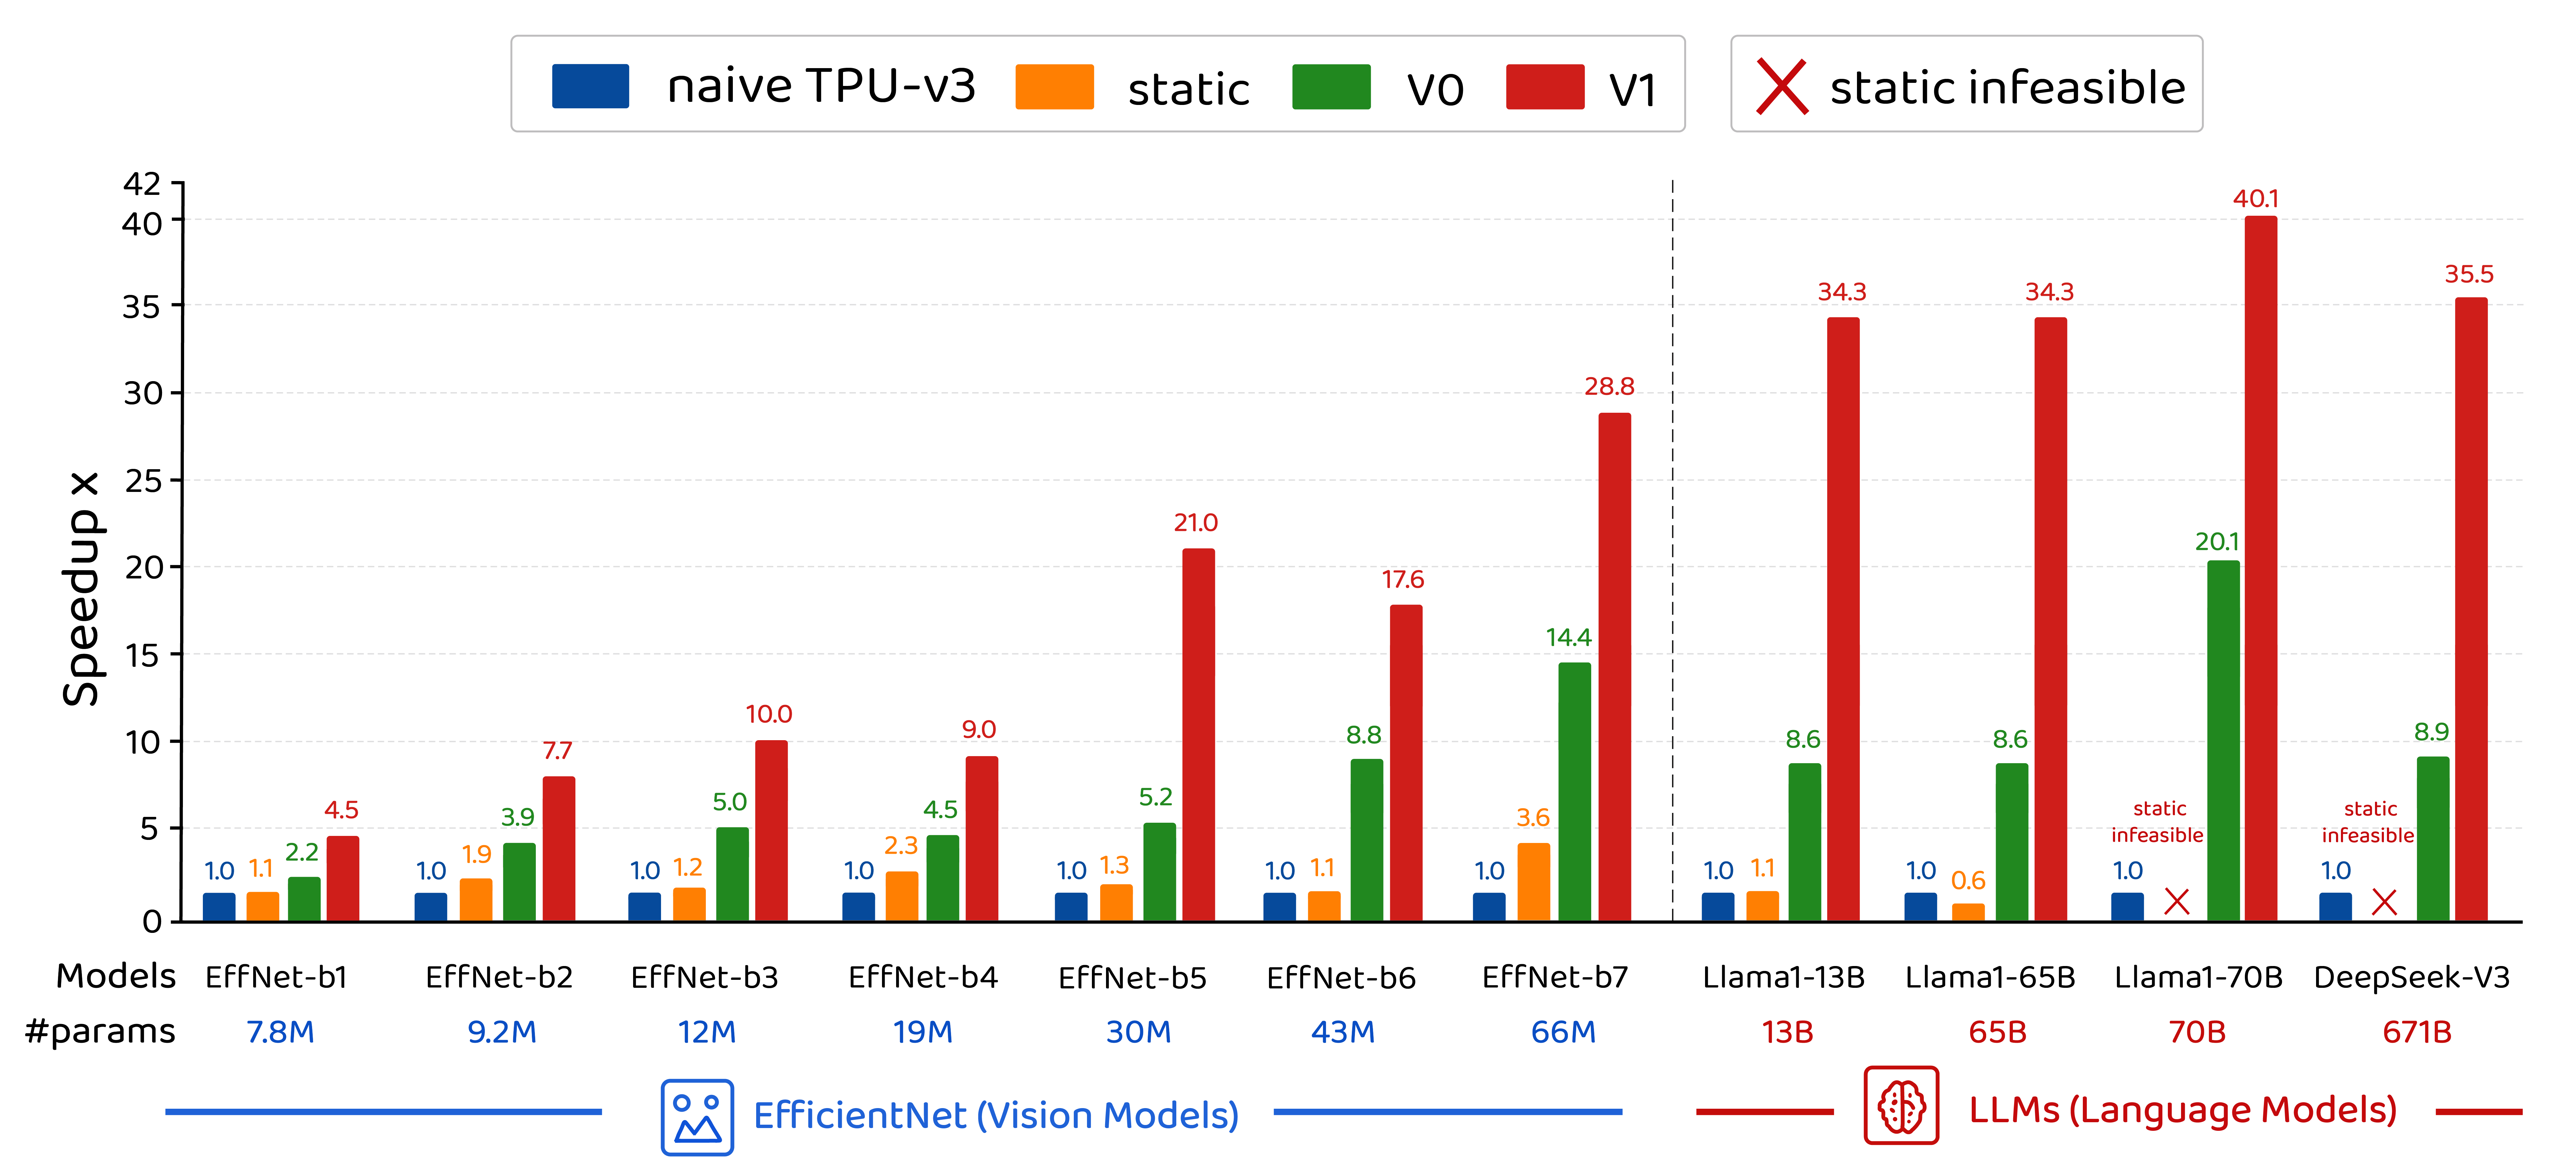
\includegraphics[width=1.0\linewidth]{fig3/speedup_final_v2.png}
% % \caption{Speedup over modeled TPU-v3 baseline across formulations and workloads: CHEETAH-V1's joint tiling-fusion optimization achieves up to $\sim$40.1$\times$ acceleration, while static fusion is infeasible on large-scale LLMs. Progressive gains are visible across formulations: V0's dynamic placement improves over static by $2$--$20\times$, while V1's joint tiling-fusion adds another $2$--$4\times$ on top. See Section~\ref{sec:experiments} for full analysis and wall-clock time breakdowns.}
% % \label{fig:speedup}
% % \end{figure}

% % % In addition to efficiently enabling more globally optimized accelerator designs, we anticipate that future work may build off this foundation to implement custom Flash Attention type speedup mechanisms for individual hardware (such as RTX5090) and workloads (such as LLama70B) tractably within hours, as well as quickly and efficiently design custom accelerators for targeted inference tasks. 
% % % compromise on any single workload; a growing body of evidence suggests that workload-specialized designs can deliver $2$--$6\times$ improvements in performance per watt.
% % % The resulting system replaces FAST's sequential Timeloop$\rightarrow$fusion~ILP pipeline with a single LP that jointly optimizes tiling, fusion, and memory scheduling, while preserving Vizier's outer loop over hardware configurations (or replacing it with LLM-guided search).

% % % Furthermore, FAST's fusion ILP uses static tensor placement: a tensor is either pinned for the entire inference pass or not at all.
% % % This is overly conservative for models with long dependency chains or skip connections, where different tensors are live at different times during execution.
% % % A dynamic placement strategy that can evict and re-pin tensors across timesteps could substantially improve global memory utilization. Joint Optimization is the only way to solve the "Memory Wall" for large scale models like DeepSeek-V3.

% % % FAST operates via a three-stage sequential pipeline (Figure \ref{fig::workflow}): (1)~a black-box optimizer (Google Vizier \citep{google_vizier}) proposes a hardware configuration defined by 16 hyperparameters---PE grid dimensions, systolic array sizes, buffer capacities, DRAM channels, and batch size; (2)~a scheduling engine (Timeloop \citep{timeloop}) finds the best tiling and mapping for each operation independently given the fixed hardware; and (3)~an integer linear program (ILP) decides which tensors to pin in the on-chip Global Memory to reduce DRAM traffic.
% % % The result of each trial---predicted performance per TDP---is fed back to Vizier, which proposes the next hardware configuration, repeating for thousands of trials until convergence.


% % % automate the framework with SkyDiscover Loop for profile and context aware co-design. Therefore in less than five hours, we are able to find an more performant design spec than the strongest baseline on designing , in terms of both perf/TDP and speedup. Our experiments also include freezing any hardware at input, and reducing the scheduling, tiling, etc search to just the LP can yield speedups of avg 2.2x than just the base hardware along. We anticipate that future work may build off this foundation to implement custom Flash Attention type speedup mechanisms for individual hardware (such as RTX5090) and workloads (such as LLama70B) tractably within hours. 

% % % Our propose the formulation for global co-design for a custom accelerator as a large scale linear program which captures strict dependencies and tradeoffs sequential methods may miss. Our LP formulation captures scheduling, tiling, rematerialization, and is able to solve matrices at scales of $6{,}319 \times 4{,}516$,\ nnz$=829{,}852$ \& $3{,}669{,}793 \times 3{,}263{,}443$,\ nnz$=7{,}342{,}293$ \& $2{,}983{,}450 \times 2{,}504{,}019$,\ nnz$=6{,}094{,}156$ quickly, by utilizing a JAX based large scale solver. Our insight is that despite the challenging large scale of the problem, the structure of the matrices, once formed, retain the same structure. Therefore we are able to design one preconditioning scheme to these large scale systems matrices that can be re-used across any NN. This also allows us to capture dependencies prior methods cannot, for example our formulation introduces a dynamic placement strategy that can evict and re-pin tensors across timesteps could substantially improve global memory utilization. Joint Optimization is the only way to solve the "Memory Wall" for large scale models like DeepSeek-V3. 

% % % For EfficientNet-B7 at $L=400$ operations and $T=400$ timesteps, the V1 LP contains approximately $2$ million variables and $5$ million constraints with $15$--$25$ million nonzeros. To better solve such large-scale LP problems more efficiently, we implement our own variant of a GPU-accelerated solver based on recent primal-dual LP algorithm \citep{applegate2022practicallargescalelinearprogramming}. We extend its original formulation in various ways and benchmark our implementation compared to existing commercial SciPy solvers, which showcase the advantage of our solver. To keep the main context clean and focused, we defer LP solver-related details to Appendix \ref{app:solver}.

% % % A large number of black box optimization tools to handle this large search space have been recently proposed, such as Google's Vizier, Meta's AX, and Optuna. In addition search strategies are also explored, for example Google's Vizier proposes numerous methods Gaussian Process Upper Confidence Bound, Eagle Strategy as a metaheuristic optimization algorithm designed for global optimization via a two-stage hybrid approach that combines global exploration with intensive local search, and Linear Combination Swarm (LCS). However these methods share certain limitations, since they cannot globally capture the tradeoffs and tensions between sequential decisions and rely on brute force iterations. This requires human engineers to spend months of compute and thousands of repetitive trials to get improvements, without feedback on what might be globally optimal. 

% % % While this sequential decomposition makes the problem tractable, it introduces a fundamental limitation: \emph{each stage takes the previous stage's output as fixed input, preventing the discovery of solutions that require trading off across stages.} Consider a concrete example: for a depthwise-separable convolution layer in a NN, a search tool such as Timeloop might select a tiling configuration that maximizes compute utilization at $74\%$, producing an activation working set of $6$ MiB. THe stacked The downstream fusion ILP solver tool receives this fixed working set size, cannot fit the tensor into the $128$ MiB Global Memory alongside other pinned tensors. However, an alternative tiling configuration with slightly lower utilization ($70\%$) might produce a working set of only $3$ MiB, enabling the fusion solver to pin an additional weight tensor that eliminates a DRAM bottleneck entirely, thus yielding a net $>20\%$ cycle reduction despite the $4\%$ utilization loss. Therefore these sequential pipelines systematically misses such cross-stage trade-offs.

% % % The rapid evolution of deep learning workloads has created a compelling opportunity for domain-optimized inference accelerators.
% % % Production models now serve billions of daily users, and the computational demands of architectures based on depthwise-separable convolutions (EfficientNet), self-attention (BERT, LLaMA), mixture-of-experts (DeepSeek-V3, Mixtral), and state-space models (Mamba) differ dramatically in their compute-to-memory ratios, tensor shapes, and data reuse patterns. However although the NN training strategy has been scaled up and we've done a lot of work on it, we now face the inference bottle neck era since general-purpose hardware, Nvidia's gaming GPUs are not necessarily optimized for deep learning tasks, and leaves a huge amount of compute on the table.

% % refer tofigure 2 edit

% % \section{Introduction}
% % \label{sec:introduction}

% % \begin{figure}[ht!]
% %     \centering
% %     \includegraphics[width=1.0\linewidth]{figs/cheetah_v4.png}
% % \caption{Sequential vs Unified Optimization Paradigm Comparison.
% % (Left) Baseline methods decouple hardware search, operation-level tiling, and static fusion; precluding cross-stage trade-offs.
% % (Right) CHEETAH presents a unified LLM-driven LP-solver-based framework that jointly optimizes tiling, placement, and rematerialization while learning from a causal ledger.}
% % \label{fig::workflow}
% % \end{figure}
% % % The rapid evolution of deep learning workloads varies from convolutions to self-attention (LLaMA), mixture-of-experts (DeepSeek-V3), and state-space models (Mamba). These diverse architectures serve billions of daily users, and have fundamentally shifted the requirements for hardware acceleration. As foundation models continue to scale in parameters, the primary cost and bottleneck of model deployment has shifted from training to inference. Therefore much recent research has been focused on optimizing for more efficient execution and throughput across diverse, high-dimensional workloads. General-purpose GPUs remain largely designed for graphics-heavy throughput, and leave substantial efficiency and compute on the table at these tasks. Therefore we are motivated to design targeted accelerators that are optimized for handling the varying tensor shapes and data-reuse patterns of modern deep learning architectures.
% % % Much research has been done in accelerating inference through custom accelerator design, more efficient neural network (NN) batching algorithms, and domain specific packages and languages that aim to speed up general NN inference. For example, the widely adopted Flash Attention uses tiling to provide significant speedups by optimizing memory movement between SRAM and DRAM. Co-design takes this a step further by aiming to optimize hardware, software and scheduling to unlock performance neither could reach independently. The traditional framework of doing this is a sequential pipeline of heuristics tools, requiring human engineers to iterate through a large search space for months from testing for the size of DRAM, to determining higher level scheduling problems. Optimizing each piece of this complex pipeline is extremely challenging, since hardware datapaths, software schedules, and compiler transforms across a combinatorial space exceeding $\mathcal O(10^{2300})$.
% % The AI inference demand is expected to grow by $10,000\times$ over the next 5 years \citep{cra2026aifuture}. General-purpose accelerators leave significant efficiency gains unrealized, which motivates the design of targeted custom accelerators. Co-design, which jointly optimizes hardware, software, and scheduling for target workloads, offers a path to unlock performance efficiency for the upcoming inference era. However, the prevailing approach relies on sequential pipelines of heuristic tools, a slow, human-driven process navigating a combinatorial search space exceeding $O(10^{2300})$ \citep{zhang_fast}. State-of-the-art frameworks like FAST \citep{zhang_fast} improve on through an automated flow (a hardware proposer feeds an operation-level tiling agent, which feeds a downstream fusion solver), but remain fundamentally decoupled.  For example, a tiling configuration that is \textit{locally} optimal for one layer may create an activation footprint that later prevents \textit{global} fusion, while a slightly slower tiling might shrink the working set enough to eliminate a DRAM bottleneck entirely. Sequential pipelines are systematically unable to express these interactions, leading to locally good but globally sub-optimal designs.

% % % The co-design problem is increasingly important as inference efficiency is the dominant AI workload and is rapidly growing. Therefore industry leaders such as NVIDIA and Google have designed chips for improved hardware-native agentic AI and , and state-of-the-art frameworks such as FAST, address this through a sequential decomposition of heuristics (a hardware proposer feeds an operation-level tiling agent, which feeds a downstream fusion solver). While FAST-generated accelerators can provide increased speedups over baseline TPU-v3, this decoupled approach is limited since it cannot capture cross-stage trade-offs. A tiling configuration that is \textit{locally} optimal for one layer may create an activation footprint that later prevents \textit{global} fusion, while a slightly slower tiling might shrink the working set enough to eliminate a DRAM bottleneck entirely. Sequential pipelines are systematically unable to express these interactions, leading to locally good but globally sub-optimal designs. 
% % We prove that by unifying the design space into a single convex relaxation, we find global optima that were previously  infeasible. Specifically, we introduce CHEETAH: a custom inference accelerator design framework that unlocks globally optimized designs with a dual-loop engine (See Figure \ref{fig::workflow}). Our inner-loop is a novel large-scale Linear Program (LP) to precisely mathematically model strict design decisions and constraints that must not be violated. The LP captures trade-offs for targeted workloads through time-indexed placement and rematerialization, thus allowing tensors to be dynamically pinned, evicted, recomputed across inference timesteps. We further extend our reformulation to internalize tiling selection into the LP, by introducing Pareto-pruned tiling variables and the McCormick linearization (a convex relaxation used for optimization of bilinear problems \citep{mccormick1976computability}). By exploiting the structural invariance of our matrices across hardware trials, we also adapt a GPU-accelerated primal-dual solver in JAX that can resolve millions of variables to rapidly reduce trial time from days to hours. This allows the LP solver to jointly reason about hardware configuration, activation placement, and weight pinning in a single pass, while providing feedback signal via Lagrangian duals.

% % Our outer-loop framework stacks a black-box optimizer (Google Vizier \citep{google_vizier}) to propose candidate hardware configurations defined by a set of hyperparameters (e.g., processing element grid dimensions, systolic array sizes, DRAM size, etc), while a LLM is used for efficient search-space steering. The LLM acts as a causal architect, interpreting a compact trial ledger of roofline checks and LP feedback diagnostics to propose constrained architectural search input for Vizier. This prevents the search-space gaming typical of black-box optimizers in wide design regions, and reduces the need for thousands of sequential trails via Bayesian search strategies in Vizier to learn good vs bad neighborhoods in search topology. Our results demonstrate that the LLM-Architect framework further reduces invalid hardware trials from 24.5\% under vanilla Vizier to 5.9\%, while reaching the Pareto frontier 4.5x faster than the next strongest baseline. We validate all results with Model Flop Utilization (MFU)  and roofline lower-bound audits, ensuring predicted latencies are physically grounded in compute and memory throughput limits. 
% % % \todo{Add best of both worlds, strengths from principled LP side, from LLM aggregate info side}
% % % \todo{Aggregates past experience to gain insight into steering hardware-software co-design. We offload the strict solves, with constraints that must the strictly respected, to the LP solve part. This combines the best of both worlds.} 
% % \paragraph{Contributions.} We reformulated the fundamental HW/SW co-design problem into a unified  framework in CHEETAH, combining principled mathematical rigor of the LP formulation to solve strict design decisions optimally, with the powerful aggregation and causal learning of an LLM Architect outer loop for meta-optimization. Our open-source repository for full reproducibility is at \href{https://anonymous.4open.science/r/CHEETAH-B268/readme}{https://anonymous.4open.science/r/CHEETAH-B268/}.

% % \begin{enumerate}
% %     \item \textbf{CHEETAH-V0 - Dynamic Placement with Rematerialization:}
% %     We introduce the time-indexed and rematerialization variables to enable cheap recompute operations (\eg, depthwise convolutions that account for only $5\%$ of FLOPs but produce large activations) instead of paying DRAM reload costs. This addresses the restrictions of existing baseline methods where activations can only be pinned between consecutively-executed operations, and supports skip connections and multi-fanout nodes.

% %     \item \textbf{CHEETAH-V1 - Joint Tiling-Fusion:}
% %     We unify tiling and fusion into a single LP problem by introducing tiling selection variables $y_{i,c}$, and employ McCormick envelopes to exactly linearize the bilinear interaction between tiling and tensor pinning. This technique yields a tight, parameter-free LP relaxation, and the coupling internalizes the tiling-placement trade-off to discover optimal design points that sequential pipelines systematically miss.
% %     % This enables the LP to discover trade-offs where accepting a suboptimal tiling configuration enables superior fusion, or vice versa---precisely the cross-stage interactions that the sequential pipeline cannot capture.
% %     \item \textbf{LLM-guided Causal Architect:} The LLM outer loop steers hardware search and bridges high-level architectural reasoning with low-level solver duals. It interprets Lagrangian sensitivity signals to perform targeted subspace interventions, transforming black-box search into a structured, diagnostic-driven process. We use a context-aware LLM Architect to propose good search areas as input to Vizier (a black-box Bayesian optimizer). Feedback signals are aggregated across historical trials through both the Causal Ledger and the LP solver. The Architect then guides Vizier through widened search spaces, reducing invalid trials by ${\sim}4\times$ while preserving the global optimal score, while enabling profile-specific designs (speech models may emphasize latency, while data synthesis models may prioritize bandwidth). 
% %     \item \textbf{Speedup:} We show that across a large suite of vision and language modeling workloads, CHEETAH results in an average of 20.9X faster designs than prior work. 

% %     % profiles into consideration to push the black-box optimizer responsible for hardware suggestions to output with structured reasoning about architectural trade-offs. 

% % \end{enumerate}

% % We anticipate that future work may build from this framework in two ways: as an end-to-end co-design system for efficient accelerators, and as an automated optimization engine for existing hardware. By fixing the architecture, the inner loop derives optimal tiling and scheduling strategies that can act as custom speedups for targeted inference tasks.

% % % \begin{figure}[ht!] 
% % %     \centering
% % % 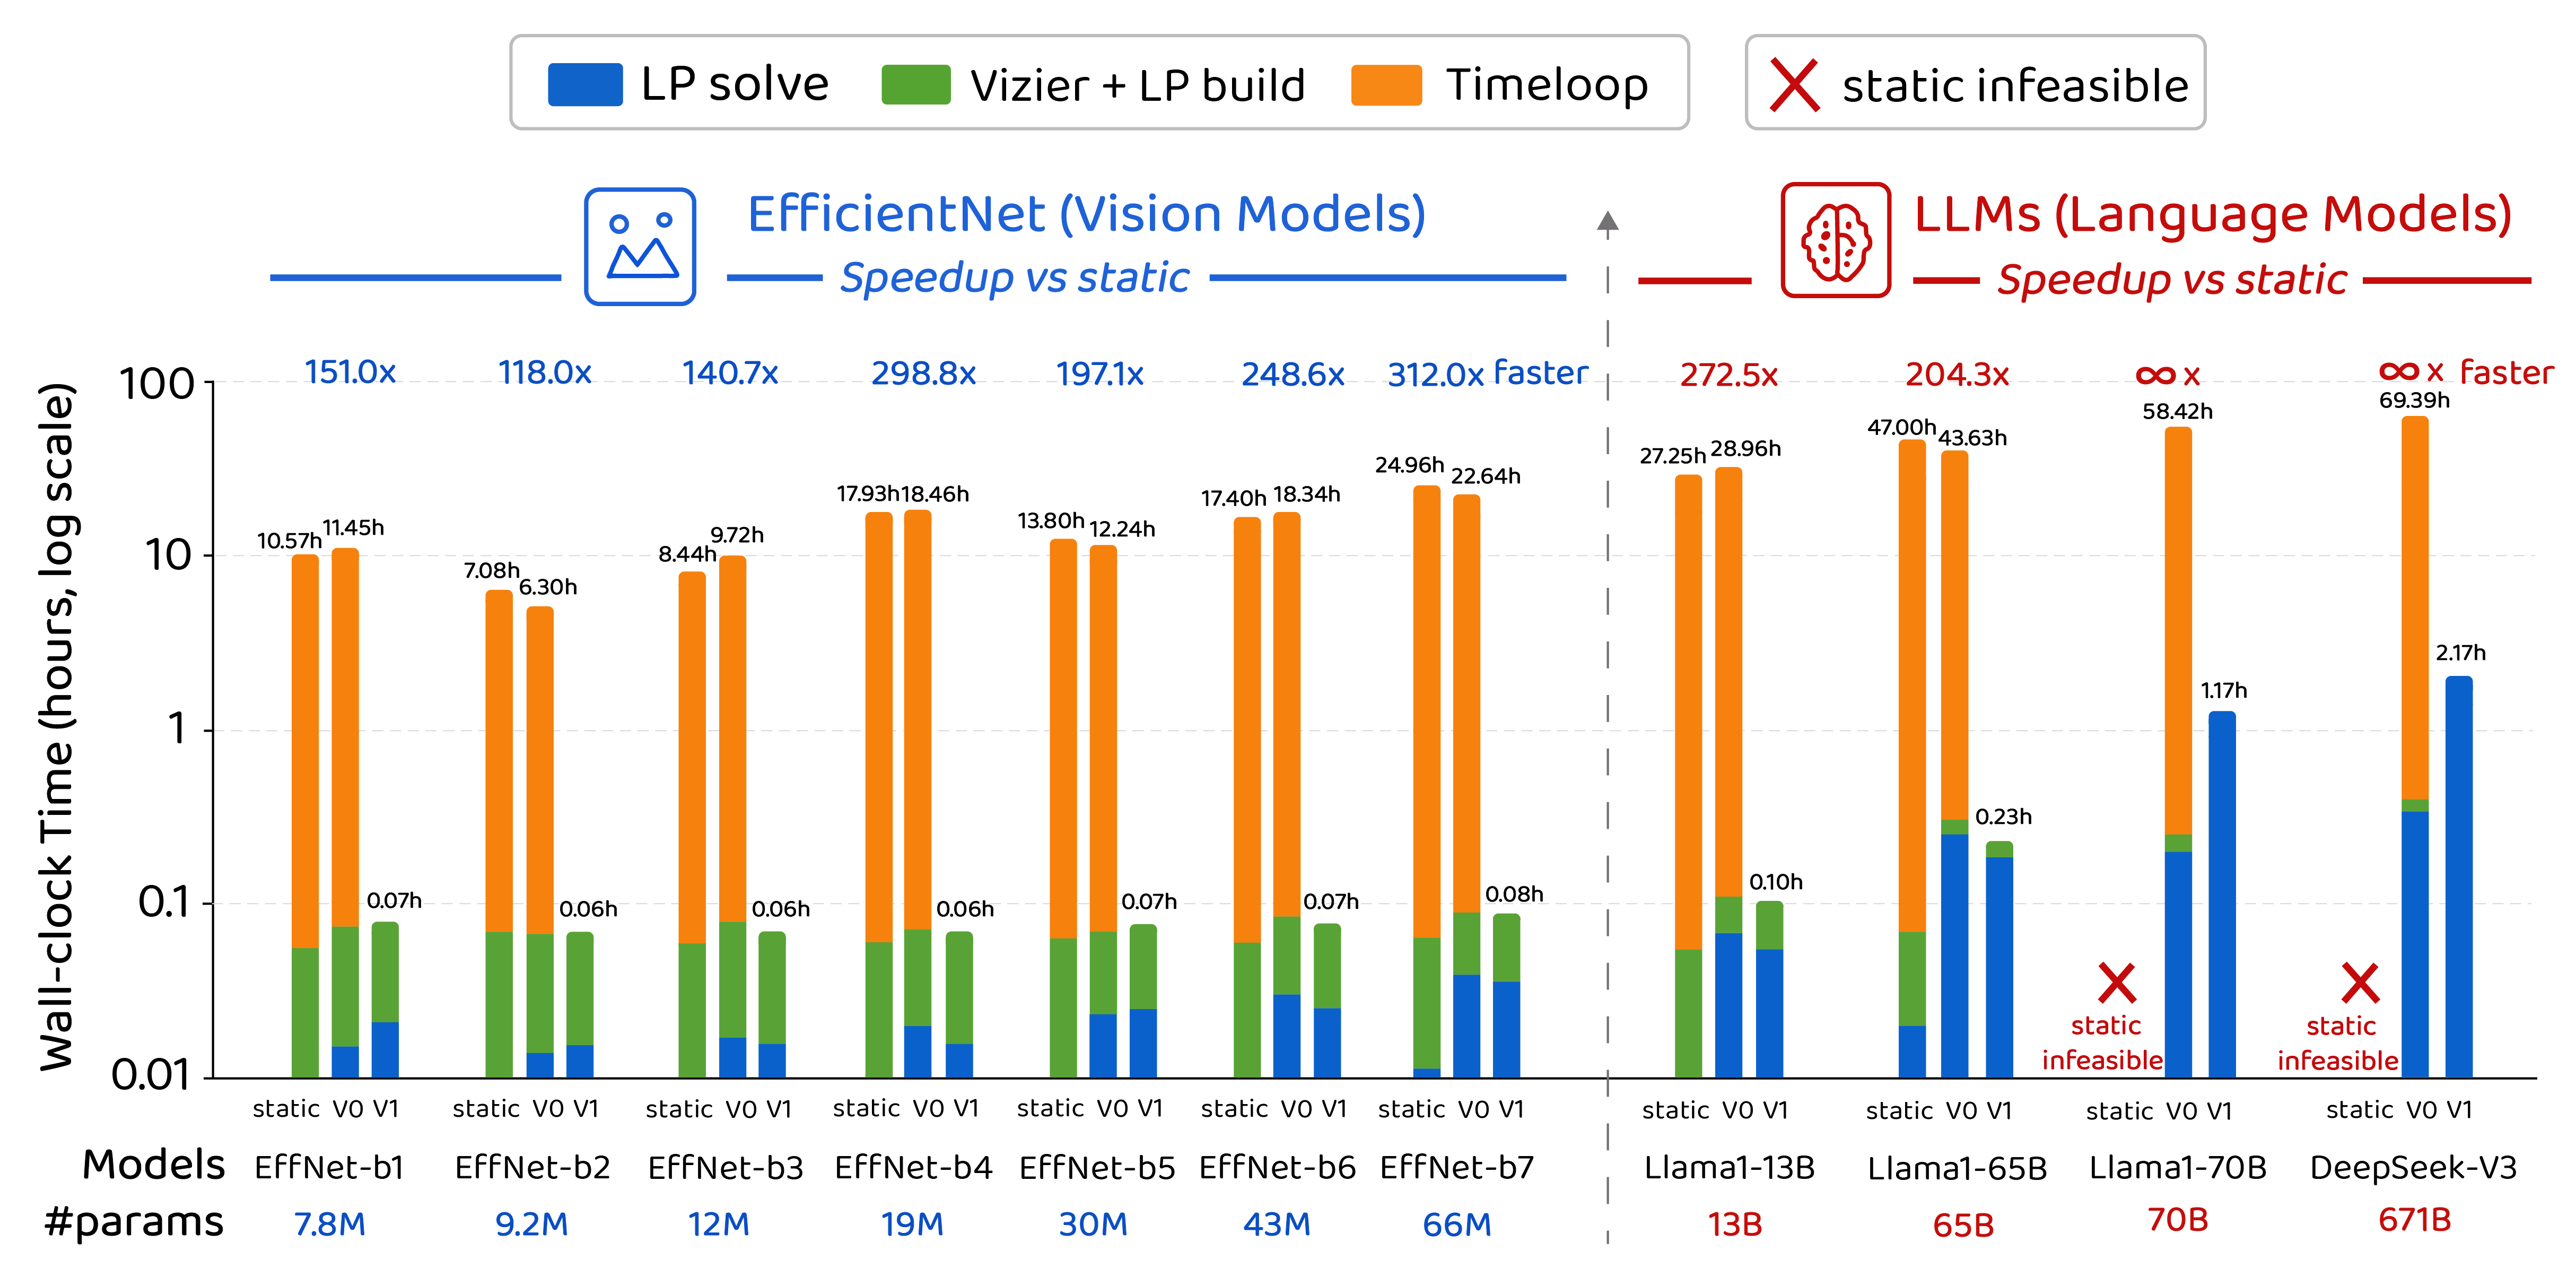
\includegraphics[width=1.0\linewidth]{fig3/wallclock_new_v5.png}
% % % \caption{Wall-clock time decomposition and performance acceleration across formulations: CHEETAH-V1's internalized tiling eliminates the Timeloop bottleneck, achieving up to 100–300× faster search than classical static method.}
% % % \label{fig:wallclock}
% % % \end{figure}

% % \begin{figure}[ht!]
% %     \centering
% % 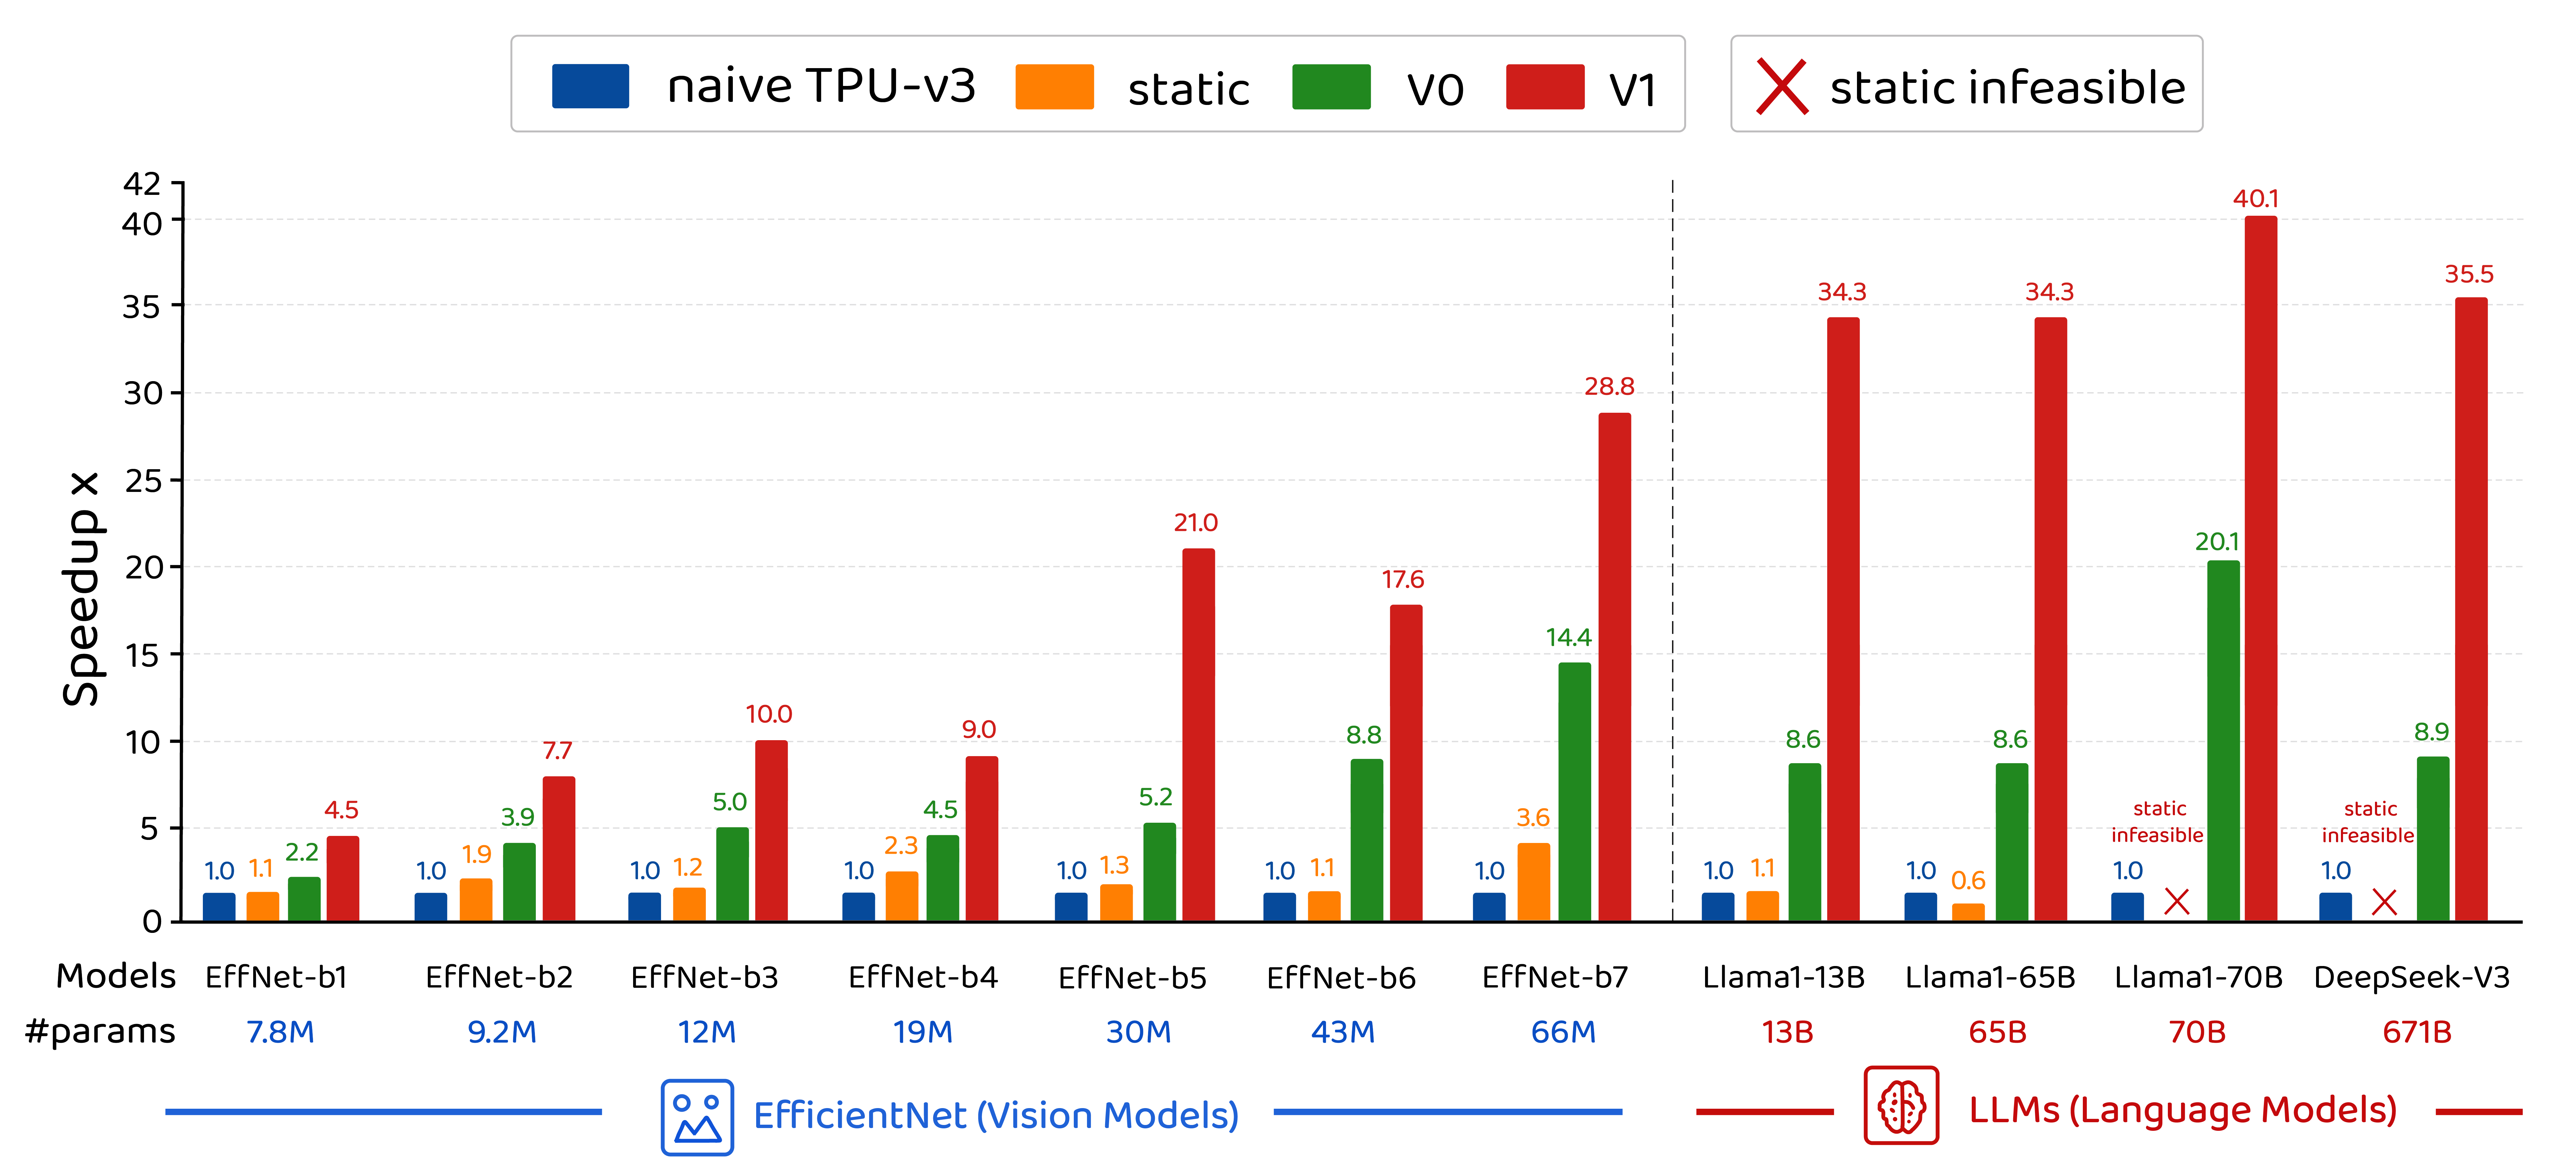
\includegraphics[width=1.0\linewidth]{fig3/speedup_final_v2.png}
% % \caption{Speedup over modeled TPU-v3 baseline across formulations and workloads: CHEETAH-V1's joint tiling-fusion optimization achieves up to $\sim$35× acceleration, while static fusion is infeasible on large-scale LLMs.}
% % \label{fig:speedup}
% % \end{figure}

% % % In addition to efficiently enabling more globally optimized accelerator designs, we anticipate that future work may build off this foundation to implement custom Flash Attention type speedup mechanisms for individual hardware (such as RTX5090) and workloads (such as LLama70B) tractably within hours, as well as quickly and efficiently design custom accelerators for targeted inference tasks. 
% % % compromise on any single workload; a growing body of evidence suggests that workload-specialized designs can deliver $2$--$6\times$ improvements in performance per watt.
% % % The resulting system replaces FAST's sequential Timeloop$\rightarrow$fusion~ILP pipeline with a single LP that jointly optimizes tiling, fusion, and memory scheduling, while preserving Vizier's outer loop over hardware configurations (or replacing it with LLM-guided search).

% % % Furthermore, FAST's fusion ILP uses static tensor placement: a tensor is either pinned for the entire inference pass or not at all.
% % % This is overly conservative for models with long dependency chains or skip connections, where different tensors are live at different times during execution.
% % % A dynamic placement strategy that can evict and re-pin tensors across timesteps could substantially improve global memory utilization. Joint Optimization is the only way to solve the "Memory Wall" for large scale models like DeepSeek-V3.

% % % FAST operates via a three-stage sequential pipeline (Figure \ref{fig::workflow}): (1)~a black-box optimizer (Google Vizier \citep{google_vizier}) proposes a hardware configuration defined by 16 hyperparameters---PE grid dimensions, systolic array sizes, buffer capacities, DRAM channels, and batch size; (2)~a scheduling engine (Timeloop \citep{timeloop}) finds the best tiling and mapping for each operation independently given the fixed hardware; and (3)~an integer linear program (ILP) decides which tensors to pin in the on-chip Global Memory to reduce DRAM traffic.
% % % The result of each trial---predicted performance per TDP---is fed back to Vizier, which proposes the next hardware configuration, repeating for thousands of trials until convergence.


% % % automate the framework with SkyDiscover Loop for profile and context aware co-design. Therefore in less than five hours, we are able to find an more performant design spec than the strongest baseline on designing , in terms of both perf/TDP and speedup. Our experiments also include freezing any hardware at input, and reducing the scheduling, tiling, etc search to just the LP can yield speedups of avg 2.2x than just the base hardware along. We anticipate that future work may build off this foundation to implement custom Flash Attention type speedup mechanisms for individual hardware (such as RTX5090) and workloads (such as LLama70B) tractably within hours. 

% % % Our propose the formulation for global co-design for a custom accelerator as a large scale linear program which captures strict dependencies and tradeoffs sequential methods may miss. Our LP formulation captures scheduling, tiling, rematerialization, and is able to solve matrices at scales of $6{,}319 \times 4{,}516$,\ nnz$=829{,}852$ \& $3{,}669{,}793 \times 3{,}263{,}443$,\ nnz$=7{,}342{,}293$ \& $2{,}983{,}450 \times 2{,}504{,}019$,\ nnz$=6{,}094{,}156$ quickly, by utilizing a JAX based large scale solver. Our insight is that despite the challenging large scale of the problem, the structure of the matrices, once formed, retain the same structure. Therefore we are able to design one preconditioning scheme to these large scale systems matrices that can be re-used across any NN. This also allows us to capture dependencies prior methods cannot, for example our formulation introduces a dynamic placement strategy that can evict and re-pin tensors across timesteps could substantially improve global memory utilization. Joint Optimization is the only way to solve the "Memory Wall" for large scale models like DeepSeek-V3. 

% % % For EfficientNet-B7 at $L=400$ operations and $T=400$ timesteps, the V1 LP contains approximately $2$ million variables and $5$ million constraints with $15$--$25$ million nonzeros. To better solve such large-scale LP problems more efficiently, we implement our own variant of a GPU-accelerated solver based on recent primal-dual LP algorithm \citep{applegate2022practicallargescalelinearprogramming}. We extend its original formulation in various ways and benchmark our implementation compared to existing commercial SciPy solvers, which showcase the advantage of our solver. To keep the main context clean and focused, we defer LP solver-related details to Appendix \ref{app:solver}.

% % % A large number of black box optimization tools to handle this large search space have been recently proposed, such as Google's Vizier, Meta's AX, and Optuna. In addition search strategies are also explored, for example Google's Vizier proposes numerous methods Gaussian Process Upper Confidence Bound, Eagle Strategy as a metaheuristic optimization algorithm designed for global optimization via a two-stage hybrid approach that combines global exploration with intensive local search, and Linear Combination Swarm (LCS). However these methods share certain limitations, since they cannot globally capture the tradeoffs and tensions between sequential decisions and rely on brute force iterations. This requires human engineers to spend months of compute and thousands of repetitive trials to get improvements, without feedback on what might be globally optimal. 

% % % While this sequential decomposition makes the problem tractable, it introduces a fundamental limitation: \emph{each stage takes the previous stage's output as fixed input, preventing the discovery of solutions that require trading off across stages.} Consider a concrete example: for a depthwise-separable convolution layer in a NN, a search tool such as Timeloop might select a tiling configuration that maximizes compute utilization at $74\%$, producing an activation working set of $6$ MiB. THe stacked The downstream fusion ILP solver tool receives this fixed working set size, cannot fit the tensor into the $128$ MiB Global Memory alongside other pinned tensors. However, an alternative tiling configuration with slightly lower utilization ($70\%$) might produce a working set of only $3$ MiB, enabling the fusion solver to pin an additional weight tensor that eliminates a DRAM bottleneck entirely, thus yielding a net $>20\%$ cycle reduction despite the $4\%$ utilization loss. Therefore these sequential pipelines systematically misses such cross-stage trade-offs.

% % % The rapid evolution of deep learning workloads has created a compelling opportunity for domain-optimized inference accelerators.
% % % Production models now serve billions of daily users, and the computational demands of architectures based on depthwise-separable convolutions (EfficientNet), self-attention (BERT, LLaMA), mixture-of-experts (DeepSeek-V3, Mixtral), and state-space models (Mamba) differ dramatically in their compute-to-memory ratios, tensor shapes, and data reuse patterns. However although the NN training strategy has been scaled up and we've done a lot of work on it, we now face the inference bottle neck era since general-purpose hardware, Nvidia's gaming GPUs are not necessarily optimized for deep learning tasks, and leaves a huge amount of compute on the table.


% % page edit

% \section{Introduction}
% \label{sec:introduction}

% \begin{figure}[ht!]
%     \centering
%     \includegraphics[width=1.0\linewidth]{figs/cheetah_v4.png}
%     % \caption{\textbf{FAST vs.\ FAST-CORGI pipeline comparison.} 
% \caption{Sequential vs Our Unified Optimization Paradigm.
% (Left) Baseline methods decouple hardware search, operation-level tiling, and static fusion; precluding cross-stage trade-offs.
% (Right) CHEETAH presents a unified LLM-driven LP-solver-based framework that jointly optimizes tiling, placement, and rematerialization while learning from a causal ledger.}
% \label{fig::workflow}
% \end{figure}
% % The rapid evolution of deep learning workloads varies from convolutions to self-attention (LLaMA), mixture-of-experts (DeepSeek-V3), and state-space models (Mamba). These diverse architectures serve billions of daily users, and have fundamentally shifted the requirements for hardware acceleration. As foundation models continue to scale in parameters, the primary cost and bottleneck of model deployment has shifted from training to inference. Therefore much recent research has been focused on optimizing for more efficient execution and throughput across diverse, high-dimensional workloads. General-purpose GPUs remain largely designed for graphics-heavy throughput, and leave substantial efficiency and compute on the table at these tasks. Therefore we are motivated to design targeted accelerators that are optimized for handling the varying tensor shapes and data-reuse patterns of modern deep learning architectures.
% % Much research has been done in accelerating inference through custom accelerator design, more efficient neural network (NN) batching algorithms, and domain specific packages and languages that aim to speed up general NN inference. For example, the widely adopted Flash Attention uses tiling to provide significant speedups by optimizing memory movement between SRAM and DRAM. Co-design takes this a step further by aiming to optimize hardware, software and scheduling to unlock performance neither could reach independently. The traditional framework of doing this is a sequential pipeline of heuristics tools, requiring human engineers to iterate through a large search space for months from testing for the size of DRAM, to determining higher level scheduling problems. Optimizing each piece of this complex pipeline is extremely challenging, since hardware datapaths, software schedules, and compiler transforms across a combinatorial space exceeding $\mathcal O(10^{2300})$.
% The AI inference demand is expected to grow by $10,000\times$ over the next 5 years \citep{cra2026aifuture}. General-purpose accelerators leave significant efficiency gains unrealized, which motivates the design of targeted custom accelerators. Co-design, which jointly optimizes hardware-software (HW/SW), and scheduling for target workloads, offers a path to unlock performance efficiency for the upcoming inference era. However, the prevailing approach relies on sequential pipelines of heuristic tools, a slow, human-driven process navigating a combinatorial search space exceeding $O(10^{2300})$ \citep{zhang_fast}. State-of-the-art frameworks like FAST \citep{zhang_fast} improve on this through an automated flow (a hardware proposer feeds an operation-level tiling agent, which feeds a downstream fusion solver), but remain fundamentally decoupled: a tiling that slightly reduces compute efficiency may shrink the working set enough to eliminate a DRAM bottleneck, yet sequential pipelines cannot discover such cross-stage trade-offs.

% % The co-design problem is increasingly important as inference efficiency is the dominant AI workload and is rapidly growing. Therefore industry leaders such as NVIDIA and Google have designed chips for improved hardware-native agentic AI and , and state-of-the-art frameworks such as FAST, address this through a sequential decomposition of heuristics (a hardware proposer feeds an operation-level tiling agent, which feeds a downstream fusion solver). While FAST-generated accelerators can provide increased speedups over baseline TPU-v3, this decoupled approach is limited since it cannot capture cross-stage trade-offs. A tiling configuration that is \textit{locally} optimal for one layer may create an activation footprint that later prevents \textit{global} fusion, while a slightly slower tiling might shrink the working set enough to eliminate a DRAM bottleneck entirely. Sequential pipelines are systematically unable to express these interactions, leading to locally good but globally sub-optimal designs. 
% Unifying the design space into a single convex relaxation yields previously infeasible global optima. Specifically, we introduce CHEETAH: a custom inference accelerator design framework that unlocks globally optimized designs with a dual-loop. Our inner-loop is a novel large-scale Linear Program (LP) to precisely mathematically model strict design decisions and constraints that must not be violated. The LP captures trade-offs for targeted workloads through time-indexed placement and rematerialization, thus allowing tensors to be dynamically pinned, evicted, recomputed across inference timesteps. We further extend our reformulation to internalize tiling selection into the LP, by introducing Pareto-pruned tiling variables and the McCormick linearization (a convex relaxation used for optimization of bilinear problems \citep{mccormick1976computability}). By exploiting the structural invariance of our matrices across hardware trials, we also adapt a GPU-accelerated primal-dual solver in JAX \citep{jax2018github} that can resolve millions of variables to rapidly reduce trial time from days to hours. This allows the LP solver to jointly reason about hardware configuration, activation placement, and weight pinning in a single pass, while providing feedback signal via Lagrangian duals.

% Our outer-loop framework stacks a black-box optimizer (Google Vizier \citep{google_vizier}) to propose candidate hardware configurations defined by a set of hyperparameters (e.g., processing element grid dimensions, systolic array sizes, DRAM size, etc), while a LLM is used for efficient search-space steering. The LLM acts as a causal architect, interpreting a compact trial ledger of roofline checks and LP feedback diagnostics to propose constrained architectural search input for Vizier. This prevents the search-space gaming typical of black-box optimizers in wide design regions, and reduces the need for thousands of sequential trials via Bayesian search strategies in Vizier to learn good vs bad neighborhoods in search topology. Our results demonstrate that the LLM Architect framework further reduces invalid hardware trials from 24.5\% under vanilla Vizier to 5.9\%, while reaching the Pareto frontier 4.5x faster than the next strongest baseline. We validate all results with Model Flop Utilization (MFU) and roofline lower-bound audits, ensuring predicted latencies are physically grounded in compute and memory throughput limits. 
% % \todo{Add best of both worlds, strengths from principled LP side, from LLM aggregate info side}
% % \todo{Aggregates past experience to gain insight into steering hardware-software co-design. We offload the strict solves, with constraints that must the strictly respected, to the LP solve part. This combines the best of both worlds.} 
% \paragraph{Contributions.} We reformulated the fundamental HW/SW co-design problem into a unified  framework in CHEETAH, combining principled mathematical rigor of the LP formulation to solve strict design decisions optimally, with the powerful aggregation and causal learning of an LLM Architect outer loop for meta-optimization. Our open-source repository for full reproducibility is at \href{https://anonymous.4open.science/r/CHEETAH-B268/readme}{https://anonymous.4open.science/r/CHEETAH-B268/}.

% \begin{enumerate}
%     \item \textbf{CHEETAH-V0 - Dynamic Placement with Rematerialization:}
%     We introduce time-indexed LP variables $p_{i,t}^k$ and rematerialization variables $r_{i,t}$ to enable cheap recompute operations instead of paying DRAM reload costs, supporting skip connections and multi-fanout nodes.

%     \item \textbf{CHEETAH-V1 - Joint Tiling-Fusion:}
%     We unify tiling and fusion into a single LP problem by introducing tiling selection variables $y_{i,c}$, and employ McCormick envelopes to exactly linearize the bilinear interaction between tiling and tensor pinning. This technique yields a tight, parameter-free LP relaxation, and the coupling internalizes the tiling-placement trade-off to discover optimal design points that sequential pipelines systematically miss.
%     % This enables the LP to discover trade-offs where accepting a suboptimal tiling configuration enables superior fusion, or vice versa---precisely the cross-stage interactions that the sequential pipeline cannot capture.
%     \item \textbf{LLM-guided Causal Architect:} The LLM outer loop steers hardware search by interpreting Lagrangian sensitivity signals and a Causal Ledger of past trials to perform targeted subspace interventions, transforming black-box search into a structured, diagnostic-driven process. The Architect guides Vizier through widened search spaces, reducing invalid trials by ${\sim}4\times$ while preserving the global optimal score, and enables profile-specific designs (speech models may emphasize latency, while data synthesis models may prioritize bandwidth). 
%     \item \textbf{Speedup:} Our method demonstrates an average speedup of $\sim22.07\times$ over the baseline across a wide range of $11$ vision and language models, reaching up to ${\sim}40.1\times$ on a single workload, as shown in  Figure \ref{fig:speedup} below.

%     % profiles into consideration to push the black-box optimizer responsible for hardware suggestions to output with structured reasoning about architectural trade-offs. 

% \end{enumerate}

% \begin{figure}[ht!]
%     \centering
% 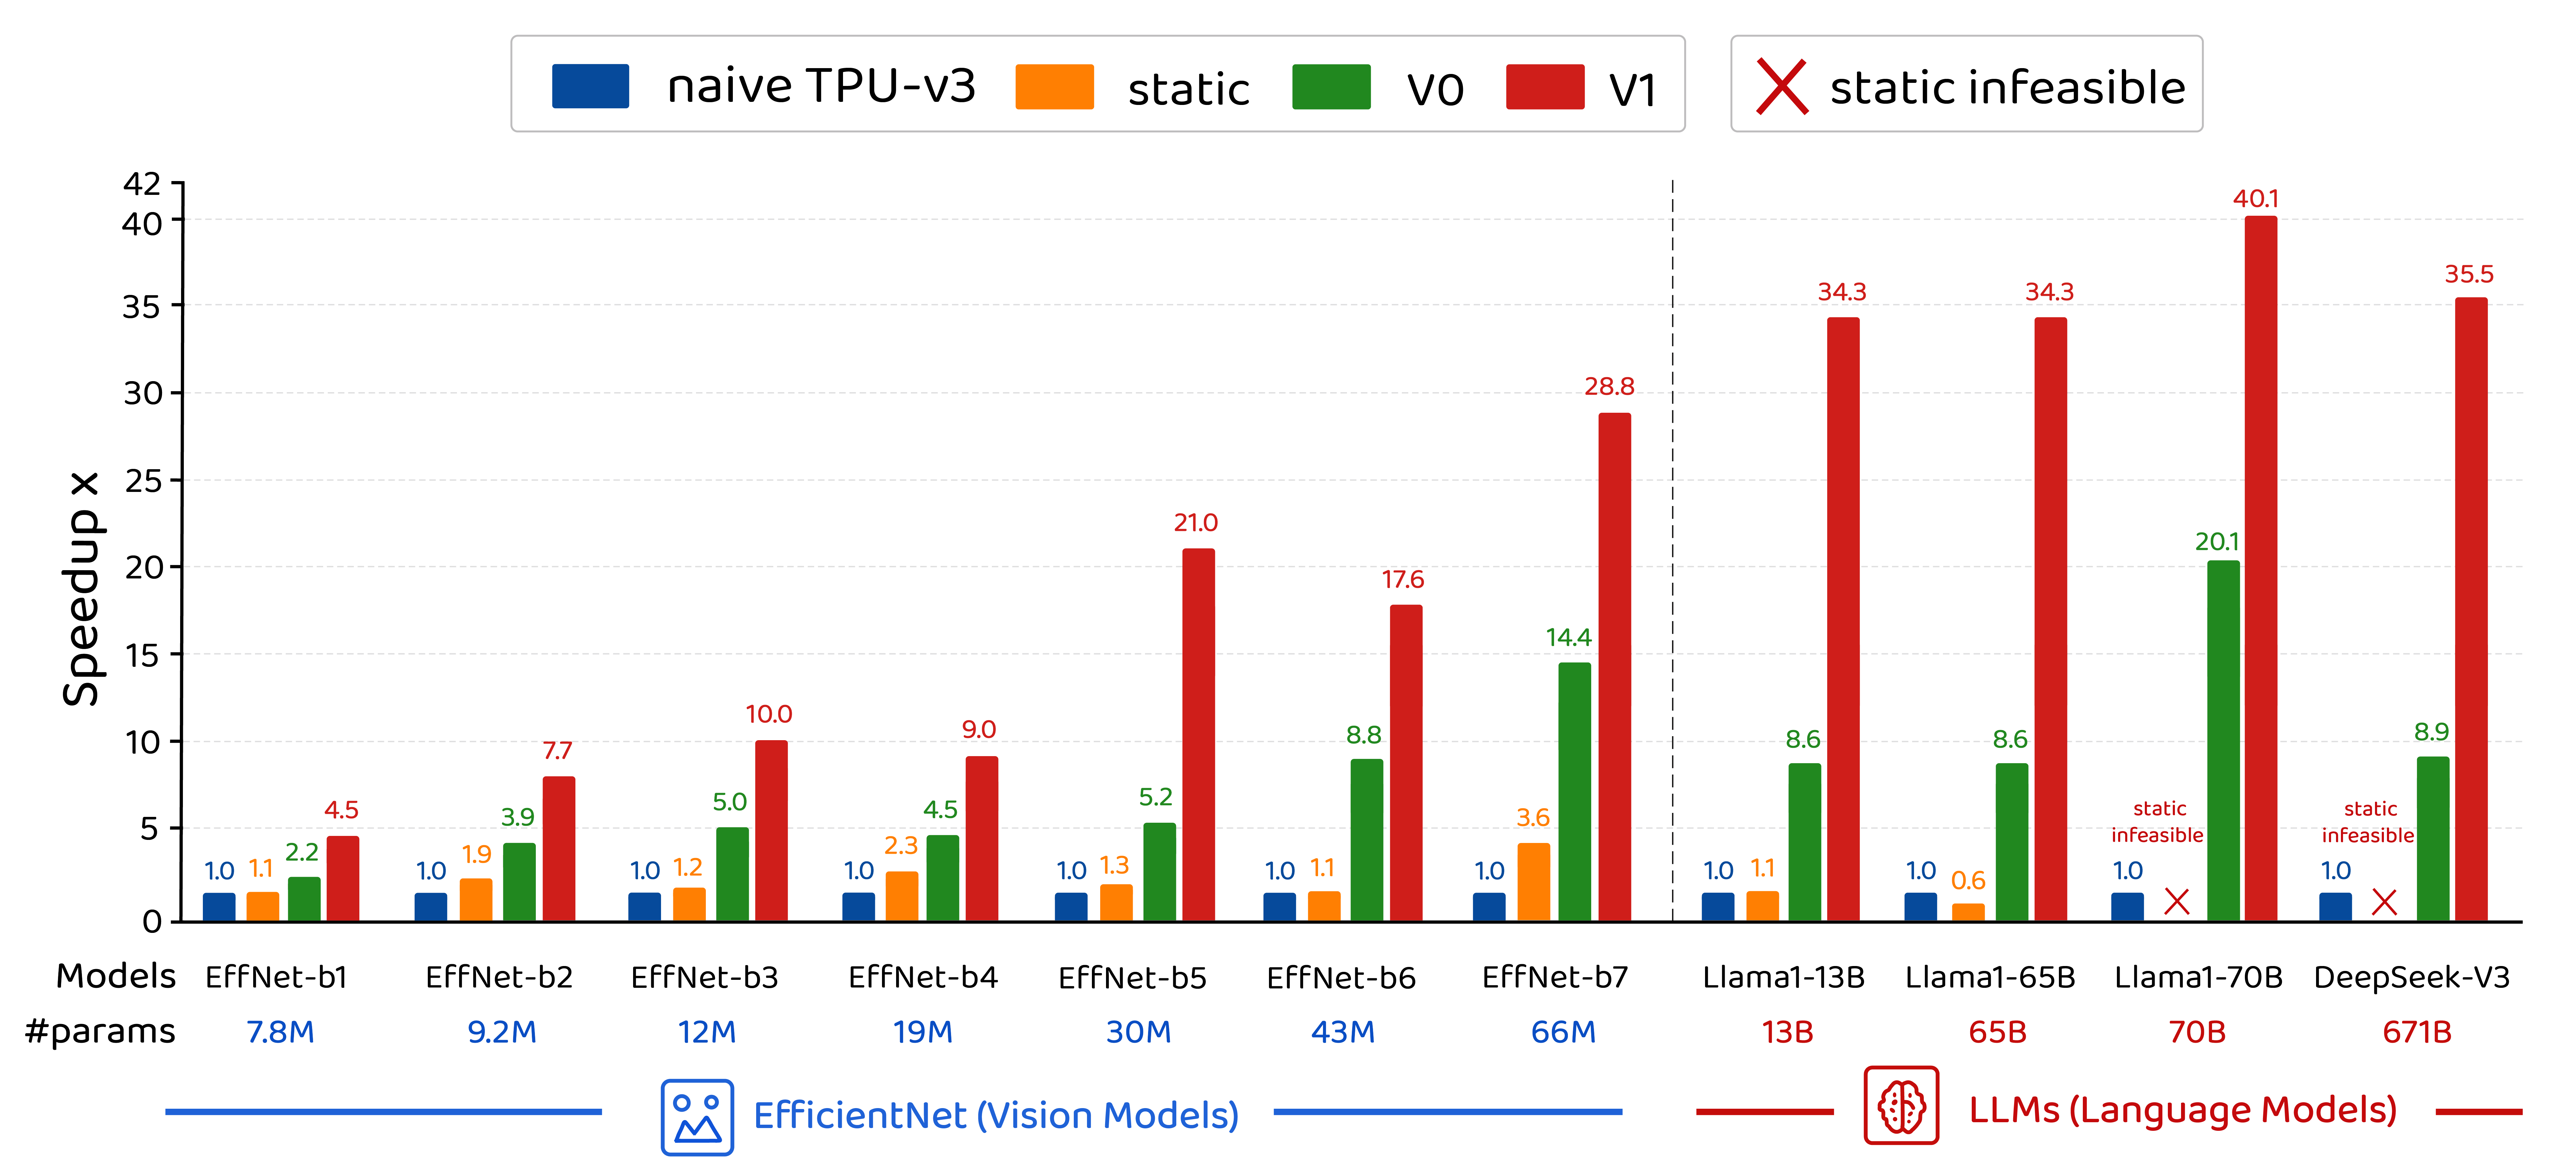
\includegraphics[width=1.0\linewidth]{fig3/speedup_final_v2.png}
% \caption{Speedup over modeled TPU-v3 baseline across formulations and workloads: CHEETAH-V1's joint tiling-fusion optimization achieves up to $\sim$40.1$\times$ acceleration, while static fusion is infeasible on large-scale LLMs. Progressive gains are visible across formulations: V0's dynamic placement improves over static by $2$--$20\times$, while V1's joint tiling-fusion adds another $2$--$4\times$ on top. See Section~\ref{sec:experiments} for full analysis and wall-clock time breakdowns.}
% \label{fig:speedup}
% \end{figure}

% % In addition to efficiently enabling more globally optimized accelerator designs, we anticipate that future work may build off this foundation to implement custom Flash Attention type speedup mechanisms for individual hardware (such as RTX5090) and workloads (such as LLama70B) tractably within hours, as well as quickly and efficiently design custom accelerators for targeted inference tasks. 
% % compromise on any single workload; a growing body of evidence suggests that workload-specialized designs can deliver $2$--$6\times$ improvements in performance per watt.
% % The resulting system replaces FAST's sequential Timeloop$\rightarrow$fusion~ILP pipeline with a single LP that jointly optimizes tiling, fusion, and memory scheduling, while preserving Vizier's outer loop over hardware configurations (or replacing it with LLM-guided search).

% % Furthermore, FAST's fusion ILP uses static tensor placement: a tensor is either pinned for the entire inference pass or not at all.
% % This is overly conservative for models with long dependency chains or skip connections, where different tensors are live at different times during execution.
% % A dynamic placement strategy that can evict and re-pin tensors across timesteps could substantially improve global memory utilization. Joint Optimization is the only way to solve the "Memory Wall" for large scale models like DeepSeek-V3.

% % FAST operates via a three-stage sequential pipeline (Figure \ref{fig::workflow}): (1)~a black-box optimizer (Google Vizier \citep{google_vizier}) proposes a hardware configuration defined by 16 hyperparameters---PE grid dimensions, systolic array sizes, buffer capacities, DRAM channels, and batch size; (2)~a scheduling engine (Timeloop \citep{timeloop}) finds the best tiling and mapping for each operation independently given the fixed hardware; and (3)~an integer linear program (ILP) decides which tensors to pin in the on-chip Global Memory to reduce DRAM traffic.
% % The result of each trial---predicted performance per TDP---is fed back to Vizier, which proposes the next hardware configuration, repeating for thousands of trials until convergence.


% % automate the framework with SkyDiscover Loop for profile and context aware co-design. Therefore in less than five hours, we are able to find an more performant design spec than the strongest baseline on designing , in terms of both perf/TDP and speedup. Our experiments also include freezing any hardware at input, and reducing the scheduling, tiling, etc search to just the LP can yield speedups of avg 2.2x than just the base hardware along. We anticipate that future work may build off this foundation to implement custom Flash Attention type speedup mechanisms for individual hardware (such as RTX5090) and workloads (such as LLama70B) tractably within hours. 

% % Our propose the formulation for global co-design for a custom accelerator as a large scale linear program which captures strict dependencies and tradeoffs sequential methods may miss. Our LP formulation captures scheduling, tiling, rematerialization, and is able to solve matrices at scales of $6{,}319 \times 4{,}516$,\ nnz$=829{,}852$ \& $3{,}669{,}793 \times 3{,}263{,}443$,\ nnz$=7{,}342{,}293$ \& $2{,}983{,}450 \times 2{,}504{,}019$,\ nnz$=6{,}094{,}156$ quickly, by utilizing a JAX based large scale solver. Our insight is that despite the challenging large scale of the problem, the structure of the matrices, once formed, retain the same structure. Therefore we are able to design one preconditioning scheme to these large scale systems matrices that can be re-used across any NN. This also allows us to capture dependencies prior methods cannot, for example our formulation introduces a dynamic placement strategy that can evict and re-pin tensors across timesteps could substantially improve global memory utilization. Joint Optimization is the only way to solve the "Memory Wall" for large scale models like DeepSeek-V3. 

% % For EfficientNet-B7 at $L=400$ operations and $T=400$ timesteps, the V1 LP contains approximately $2$ million variables and $5$ million constraints with $15$--$25$ million nonzeros. To better solve such large-scale LP problems more efficiently, we implement our own variant of a GPU-accelerated solver based on recent primal-dual LP algorithm \citep{applegate2022practicallargescalelinearprogramming}. We extend its original formulation in various ways and benchmark our implementation compared to existing commercial SciPy solvers, which showcase the advantage of our solver. To keep the main context clean and focused, we defer LP solver-related details to Appendix \ref{app:solver}.

% % A large number of black box optimization tools to handle this large search space have been recently proposed, such as Google's Vizier, Meta's AX, and Optuna. In addition search strategies are also explored, for example Google's Vizier proposes numerous methods Gaussian Process Upper Confidence Bound, Eagle Strategy as a metaheuristic optimization algorithm designed for global optimization via a two-stage hybrid approach that combines global exploration with intensive local search, and Linear Combination Swarm (LCS). However these methods share certain limitations, since they cannot globally capture the tradeoffs and tensions between sequential decisions and rely on brute force iterations. This requires human engineers to spend months of compute and thousands of repetitive trials to get improvements, without feedback on what might be globally optimal. 

% % While this sequential decomposition makes the problem tractable, it introduces a fundamental limitation: \emph{each stage takes the previous stage's output as fixed input, preventing the discovery of solutions that require trading off across stages.} Consider a concrete example: for a depthwise-separable convolution layer in a NN, a search tool such as Timeloop might select a tiling configuration that maximizes compute utilization at $74\%$, producing an activation working set of $6$ MiB. THe stacked The downstream fusion ILP solver tool receives this fixed working set size, cannot fit the tensor into the $128$ MiB Global Memory alongside other pinned tensors. However, an alternative tiling configuration with slightly lower utilization ($70\%$) might produce a working set of only $3$ MiB, enabling the fusion solver to pin an additional weight tensor that eliminates a DRAM bottleneck entirely, thus yielding a net $>20\%$ cycle reduction despite the $4\%$ utilization loss. Therefore these sequential pipelines systematically misses such cross-stage trade-offs.

% % The rapid evolution of deep learning workloads has created a compelling opportunity for domain-optimized inference accelerators.
% % Production models now serve billions of daily users, and the computational demands of architectures based on depthwise-separable convolutions (EfficientNet), self-attention (BERT, LLaMA), mixture-of-experts (DeepSeek-V3, Mixtral), and state-space models (Mamba) differ dramatically in their compute-to-memory ratios, tensor shapes, and data reuse patterns. However although the NN training strategy has been scaled up and we've done a lot of work on it, we now face the inference bottle neck era since general-purpose hardware, Nvidia's gaming GPUs are not necessarily optimized for deep learning tasks, and leaves a huge amount of compute on the table.



% figure 2 reference edit again

% \section{Introduction}
% \label{sec:introduction}

% \begin{figure}[ht!]
%     \centering
%     \includegraphics[width=1.0\linewidth]{figs/cheetah_v4.png}
% \caption{Sequential vs Unified Optimization Paradigm Comparison.
% (Left) Baseline methods decouple hardware search, operation-level tiling, and static fusion; precluding cross-stage trade-offs.
% (Right) CHEETAH presents a unified LLM-driven LP-solver-based framework that jointly optimizes tiling, placement, and rematerialization while learning from a causal ledger.}
% \label{fig::workflow}
% \end{figure}
% % The rapid evolution of deep learning workloads varies from convolutions to self-attention (LLaMA), mixture-of-experts (DeepSeek-V3), and state-space models (Mamba). These diverse architectures serve billions of daily users, and have fundamentally shifted the requirements for hardware acceleration. As foundation models continue to scale in parameters, the primary cost and bottleneck of model deployment has shifted from training to inference. Therefore much recent research has been focused on optimizing for more efficient execution and throughput across diverse, high-dimensional workloads. General-purpose GPUs remain largely designed for graphics-heavy throughput, and leave substantial efficiency and compute on the table at these tasks. Therefore we are motivated to design targeted accelerators that are optimized for handling the varying tensor shapes and data-reuse patterns of modern deep learning architectures.
% % Much research has been done in accelerating inference through custom accelerator design, more efficient neural network (NN) batching algorithms, and domain specific packages and languages that aim to speed up general NN inference. For example, the widely adopted Flash Attention uses tiling to provide significant speedups by optimizing memory movement between SRAM and DRAM. Co-design takes this a step further by aiming to optimize hardware, software and scheduling to unlock performance neither could reach independently. The traditional framework of doing this is a sequential pipeline of heuristics tools, requiring human engineers to iterate through a large search space for months from testing for the size of DRAM, to determining higher level scheduling problems. Optimizing each piece of this complex pipeline is extremely challenging, since hardware datapaths, software schedules, and compiler transforms across a combinatorial space exceeding $\mathcal O(10^{2300})$.
% The AI inference demand is expected to grow by $10,000\times$ over the next 5 years \citep{cra2026aifuture}. General-purpose accelerators leave significant efficiency gains unrealized, which motivates the design of targeted custom accelerators. Co-design, which jointly optimizes hardware, software, and scheduling for target workloads, offers a path to unlock performance efficiency for the upcoming inference era. However, the prevailing approach relies on sequential pipelines of heuristic tools, a slow, human-driven process navigating a combinatorial search space exceeding $O(10^{2300})$ \citep{zhang_fast}. State-of-the-art frameworks like FAST \citep{zhang_fast} improve on through an automated flow (a hardware proposer feeds an operation-level tiling agent, which feeds a downstream fusion solver), but remain fundamentally decoupled.  For example, a tiling configuration that is \textit{locally} optimal for one layer may create an activation footprint that later prevents \textit{global} fusion, while a slightly slower tiling might shrink the working set enough to eliminate a DRAM bottleneck entirely. Sequential pipelines are systematically unable to express these interactions, leading to locally good but globally sub-optimal designs.

% % The co-design problem is increasingly important as inference efficiency is the dominant AI workload and is rapidly growing. Therefore industry leaders such as NVIDIA and Google have designed chips for improved hardware-native agentic AI and , and state-of-the-art frameworks such as FAST, address this through a sequential decomposition of heuristics (a hardware proposer feeds an operation-level tiling agent, which feeds a downstream fusion solver). While FAST-generated accelerators can provide increased speedups over baseline TPU-v3, this decoupled approach is limited since it cannot capture cross-stage trade-offs. A tiling configuration that is \textit{locally} optimal for one layer may create an activation footprint that later prevents \textit{global} fusion, while a slightly slower tiling might shrink the working set enough to eliminate a DRAM bottleneck entirely. Sequential pipelines are systematically unable to express these interactions, leading to locally good but globally sub-optimal designs. 
% We prove that by unifying the design space into a single convex relaxation, we find global optima that were previously  infeasible. Specifically, we introduce CHEETAH: a custom inference accelerator design framework that unlocks globally optimized designs with a dual-loop engine (See Figure \ref{fig::workflow}). Our inner-loop is a novel large-scale Linear Program (LP) to precisely mathematically model strict design decisions and constraints that must not be violated. The LP captures trade-offs for targeted workloads through time-indexed placement and rematerialization, thus allowing tensors to be dynamically pinned, evicted, recomputed across inference timesteps. We further extend our reformulation to internalize tiling selection into the LP, by introducing Pareto-pruned tiling variables and the McCormick linearization (a convex relaxation used for optimization of bilinear problems \citep{mccormick1976computability}). By exploiting the structural invariance of our matrices across hardware trials, we also adapt a GPU-accelerated primal-dual solver in JAX that can resolve millions of variables to rapidly reduce trial time from days to hours. This allows the LP solver to jointly reason about hardware configuration, activation placement, and weight pinning in a single pass, while providing feedback signal via Lagrangian duals.

% Our outer-loop framework stacks a black-box optimizer (Google Vizier \citep{google_vizier}) to propose candidate hardware configurations defined by a set of hyperparameters (e.g., processing element grid dimensions, systolic array sizes, DRAM size, etc), while a LLM is used for efficient search-space steering. The LLM acts as a causal architect, interpreting a compact trial ledger of roofline checks and LP feedback diagnostics to propose constrained architectural search input for Vizier. This prevents the search-space gaming typical of black-box optimizers in wide design regions, and reduces the need for thousands of sequential trails via Bayesian search strategies in Vizier to learn good vs bad neighborhoods in search topology. Our results demonstrate that the LLM-Architect framework further reduces invalid hardware trials from 24.5\% under vanilla Vizier to 5.9\%, while reaching the Pareto frontier 4.5x faster than the next strongest baseline. We validate all results with Model Flop Utilization (MFU)  and roofline lower-bound audits, ensuring predicted latencies are physically grounded in compute and memory throughput limits. 
% % \todo{Add best of both worlds, strengths from principled LP side, from LLM aggregate info side}
% % \todo{Aggregates past experience to gain insight into steering hardware-software co-design. We offload the strict solves, with constraints that must the strictly respected, to the LP solve part. This combines the best of both worlds.} 
% \paragraph{Contributions.} We reformulated the fundamental HW/SW co-design problem into a unified  framework in CHEETAH, combining principled mathematical rigor of the LP formulation to solve strict design decisions optimally, with the powerful aggregation and causal learning of an LLM Architect outer loop for meta-optimization. Our open-source repository for full reproducibility is at \href{https://anonymous.4open.science/r/CHEETAH-B268/readme}{https://anonymous.4open.science/r/CHEETAH-B268/}.

% \begin{enumerate}
%     \item \textbf{CHEETAH-V0 - Dynamic Placement with Rematerialization:}
%     We introduce the time-indexed and rematerialization variables to enable cheap recompute operations (\eg, depthwise convolutions that account for only $5\%$ of FLOPs but produce large activations) instead of paying DRAM reload costs. This addresses the restrictions of existing baseline methods where activations can only be pinned between consecutively-executed operations, and supports skip connections and multi-fanout nodes.

%     \item \textbf{CHEETAH-V1 - Joint Tiling-Fusion:}
%     We unify tiling and fusion into a single LP problem by introducing tiling selection variables $y_{i,c}$, and employ McCormick envelopes to exactly linearize the bilinear interaction between tiling and tensor pinning. This technique yields a tight, parameter-free LP relaxation, and the coupling internalizes the tiling-placement trade-off to discover optimal design points that sequential pipelines systematically miss.
%     % This enables the LP to discover trade-offs where accepting a suboptimal tiling configuration enables superior fusion, or vice versa---precisely the cross-stage interactions that the sequential pipeline cannot capture.
%     \item \textbf{LLM-guided Causal Architect:} The LLM outer loop steers hardware search and bridges high-level architectural reasoning with low-level solver duals. It interprets Lagrangian sensitivity signals to perform targeted subspace interventions, transforming black-box search into a structured, diagnostic-driven process. We use a context-aware LLM Architect to propose good search areas as input to Vizier (a black-box Bayesian optimizer). Feedback signals are aggregated across historical trials through both the Causal Ledger and the LP solver. The Architect then guides Vizier through widened search spaces, reducing invalid trials by ${\sim}4\times$ while preserving the global optimal score, while enabling profile-specific designs (speech models may emphasize latency, while data synthesis models may prioritize bandwidth). 
%     \item \textbf{Speedup:} We show that across a large suite of vision and language modeling workloads, CHEETAH results in an average of 20.9X faster designs than prior work. 

%     % profiles into consideration to push the black-box optimizer responsible for hardware suggestions to output with structured reasoning about architectural trade-offs. 

% \end{enumerate}

% We anticipate that future work may build from this framework in two ways: as an end-to-end co-design system for efficient accelerators, and as an automated optimization engine for existing hardware. By fixing the architecture, the inner loop derives optimal tiling and scheduling strategies that can act as custom speedups for targeted inference tasks.

% % \begin{figure}[ht!] 
% %     \centering
% % 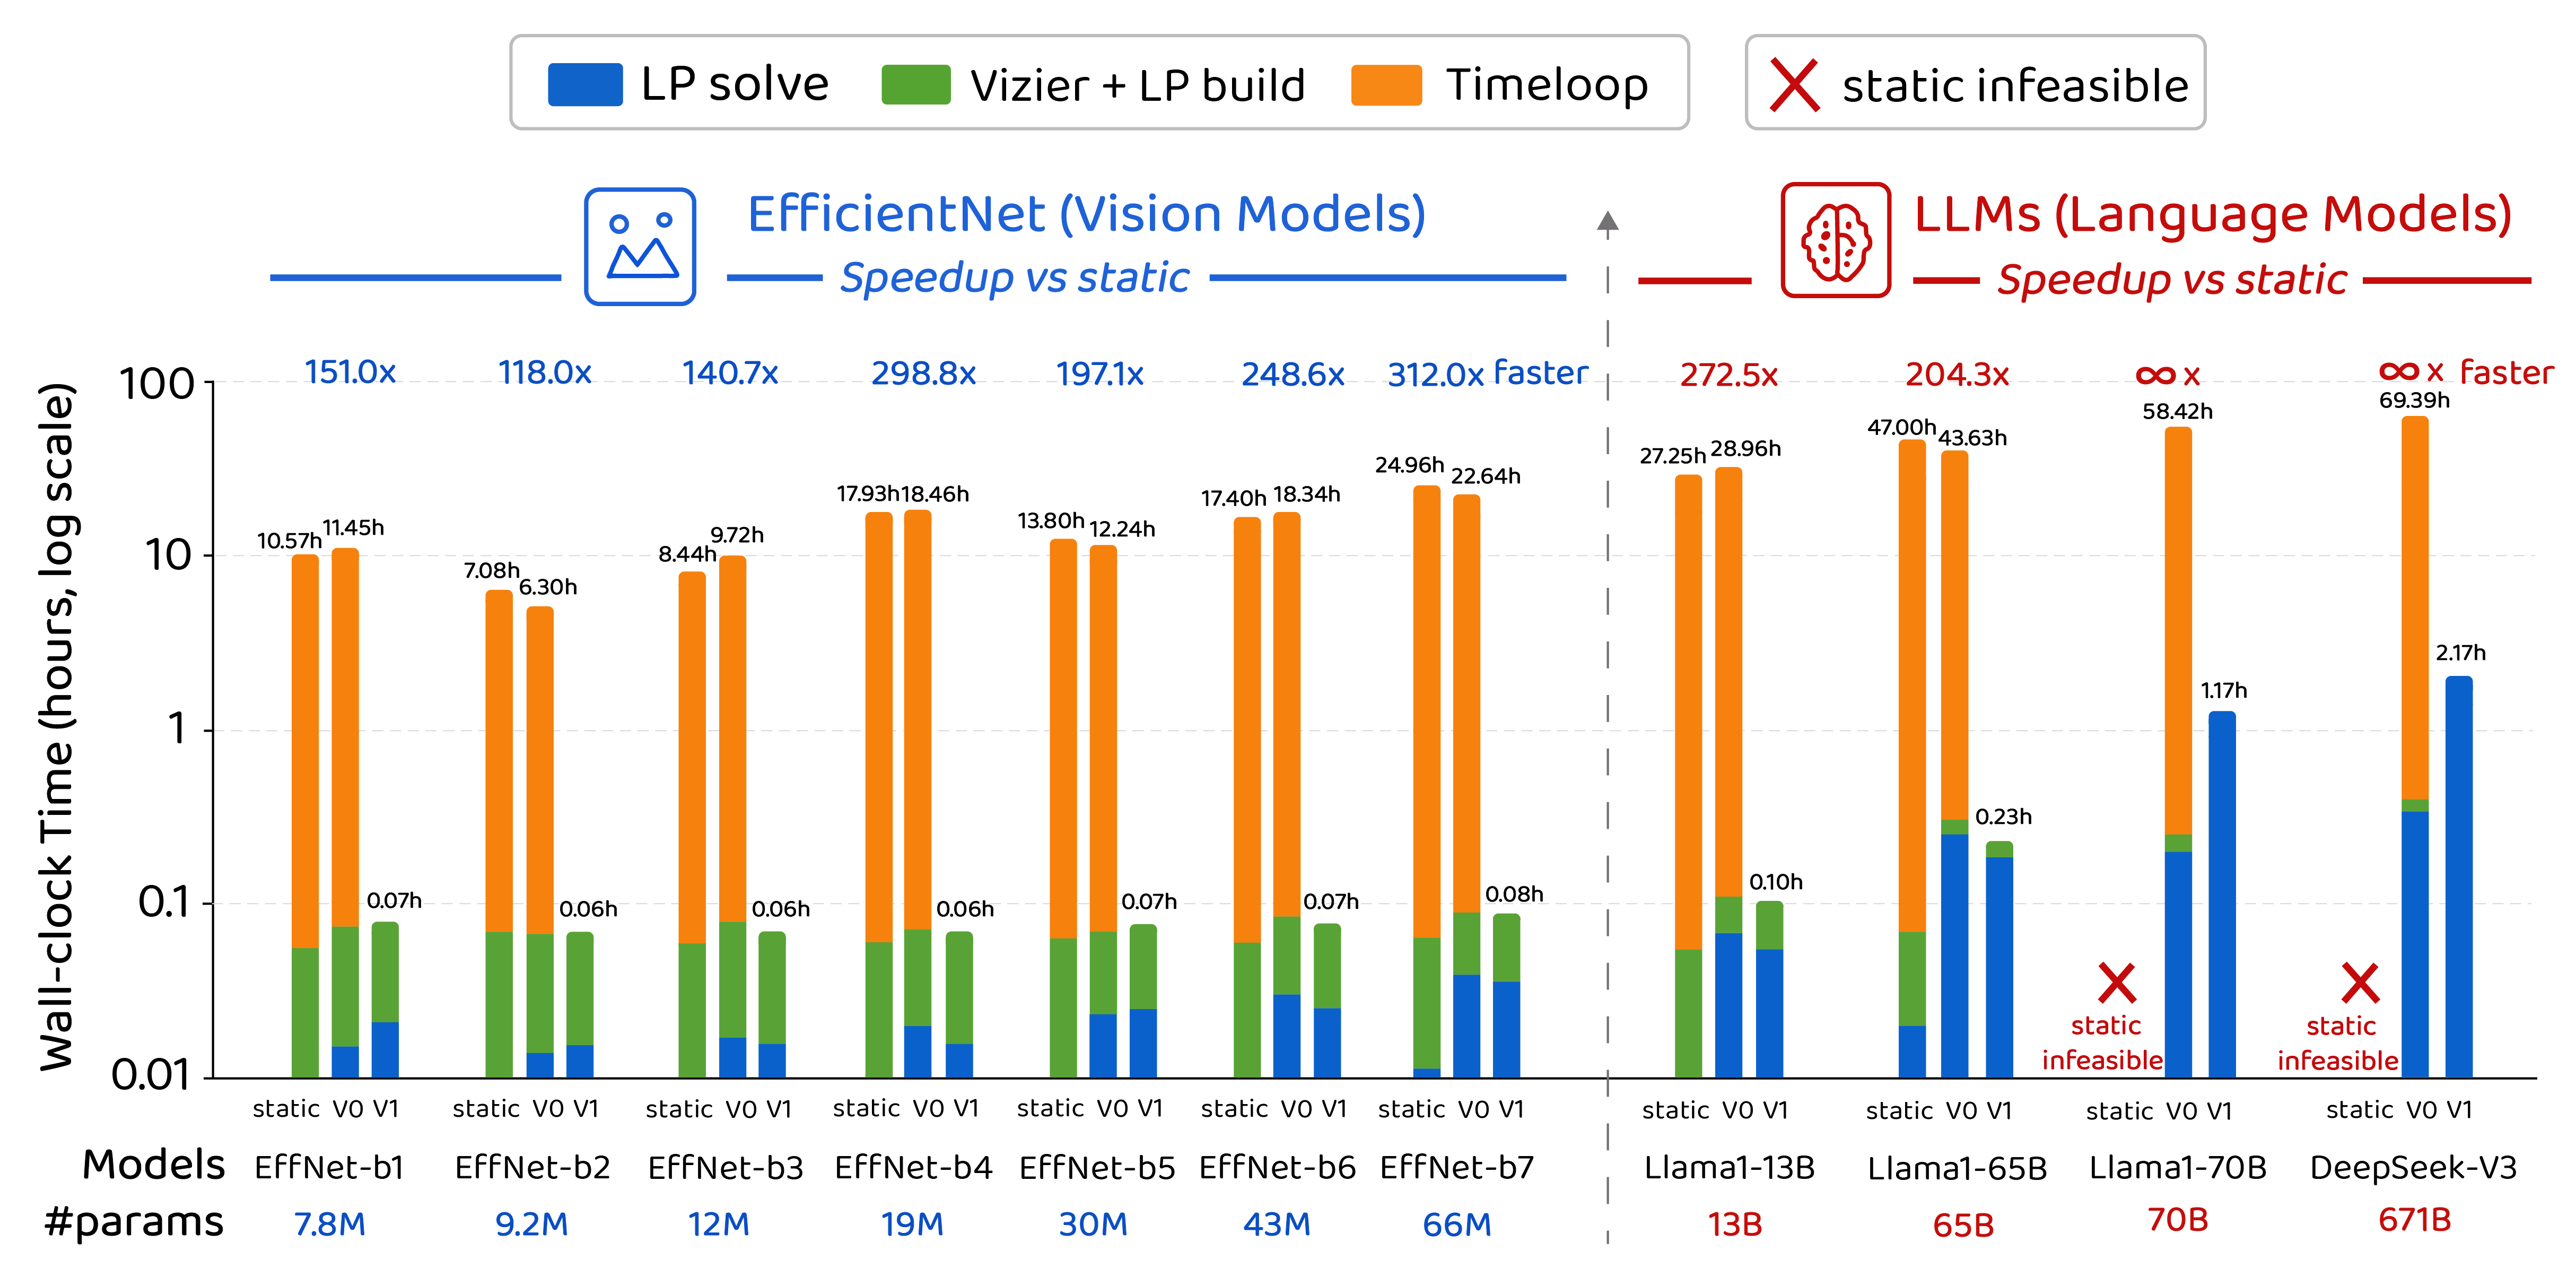
\includegraphics[width=1.0\linewidth]{fig3/wallclock_new_v5.png}
% % \caption{Wall-clock time decomposition and performance acceleration across formulations: CHEETAH-V1's internalized tiling eliminates the Timeloop bottleneck, achieving up to 100–300× faster search than classical static method.}
% % \label{fig:wallclock}
% % \end{figure}

% \begin{figure}[ht!]
%     \centering
% 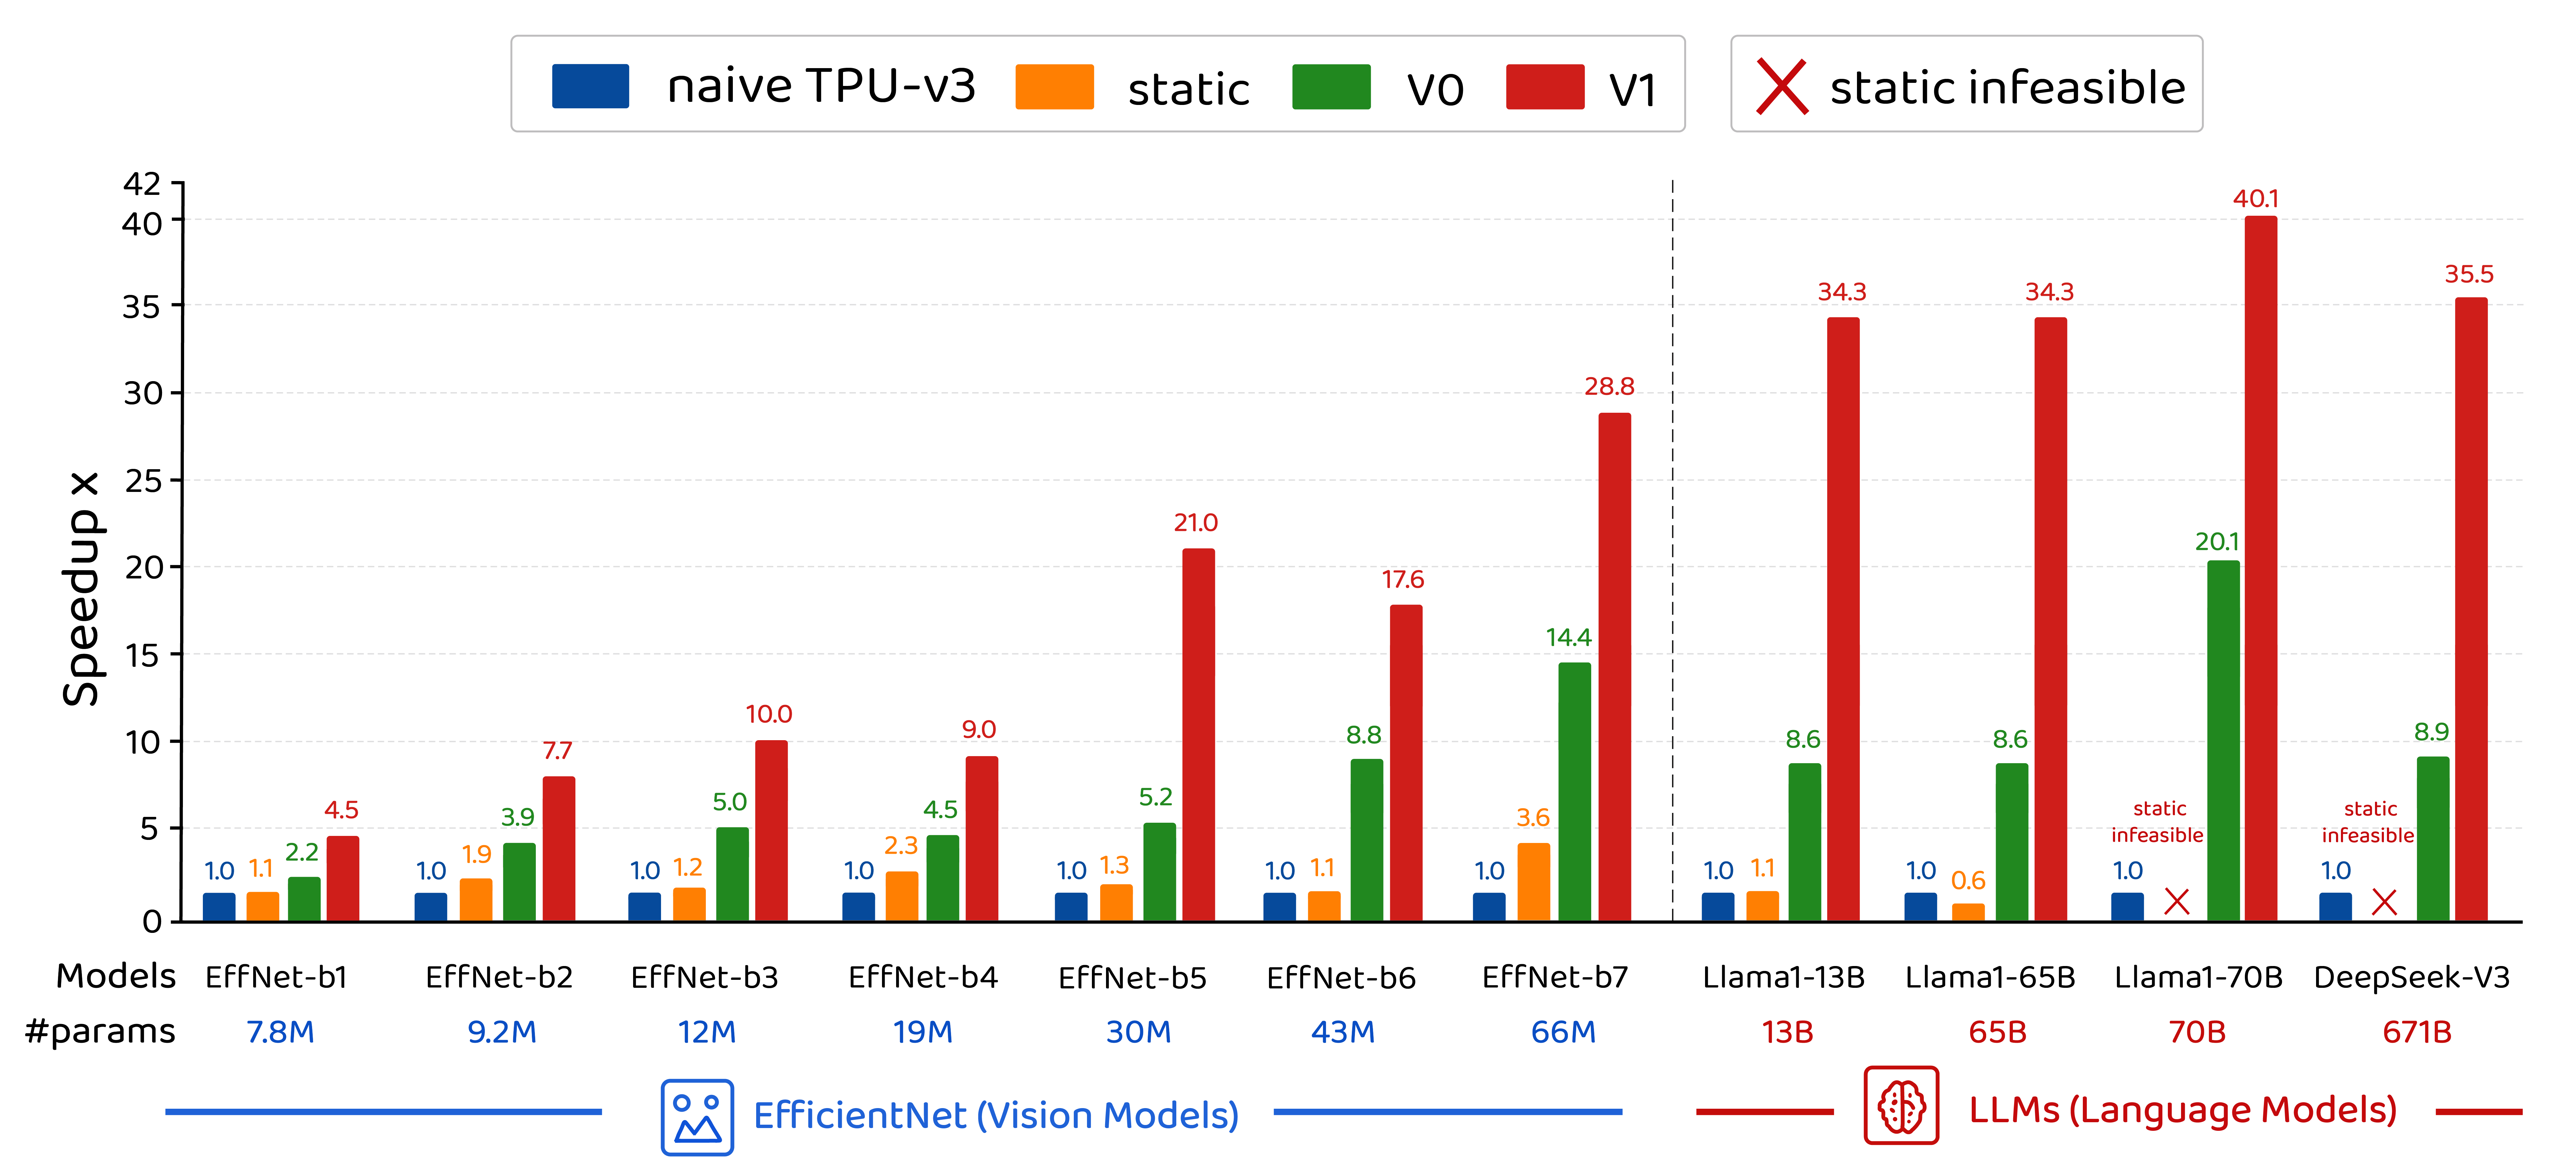
\includegraphics[width=1.0\linewidth]{fig3/speedup_final_v2.png}
% \caption{Speedup over modeled TPU-v3 baseline across formulations and workloads: CHEETAH-V1's joint tiling-fusion optimization achieves up to $\sim$35× acceleration, while static fusion is infeasible on large-scale LLMs.}
% \label{fig:speedup}
% \end{figure}

% % In addition to efficiently enabling more globally optimized accelerator designs, we anticipate that future work may build off this foundation to implement custom Flash Attention type speedup mechanisms for individual hardware (such as RTX5090) and workloads (such as LLama70B) tractably within hours, as well as quickly and efficiently design custom accelerators for targeted inference tasks. 
% % compromise on any single workload; a growing body of evidence suggests that workload-specialized designs can deliver $2$--$6\times$ improvements in performance per watt.
% % The resulting system replaces FAST's sequential Timeloop$\rightarrow$fusion~ILP pipeline with a single LP that jointly optimizes tiling, fusion, and memory scheduling, while preserving Vizier's outer loop over hardware configurations (or replacing it with LLM-guided search).

% % Furthermore, FAST's fusion ILP uses static tensor placement: a tensor is either pinned for the entire inference pass or not at all.
% % This is overly conservative for models with long dependency chains or skip connections, where different tensors are live at different times during execution.
% % A dynamic placement strategy that can evict and re-pin tensors across timesteps could substantially improve global memory utilization. Joint Optimization is the only way to solve the "Memory Wall" for large scale models like DeepSeek-V3.

% % FAST operates via a three-stage sequential pipeline (Figure \ref{fig::workflow}): (1)~a black-box optimizer (Google Vizier \citep{google_vizier}) proposes a hardware configuration defined by 16 hyperparameters---PE grid dimensions, systolic array sizes, buffer capacities, DRAM channels, and batch size; (2)~a scheduling engine (Timeloop \citep{timeloop}) finds the best tiling and mapping for each operation independently given the fixed hardware; and (3)~an integer linear program (ILP) decides which tensors to pin in the on-chip Global Memory to reduce DRAM traffic.
% % The result of each trial---predicted performance per TDP---is fed back to Vizier, which proposes the next hardware configuration, repeating for thousands of trials until convergence.


% % automate the framework with SkyDiscover Loop for profile and context aware co-design. Therefore in less than five hours, we are able to find an more performant design spec than the strongest baseline on designing , in terms of both perf/TDP and speedup. Our experiments also include freezing any hardware at input, and reducing the scheduling, tiling, etc search to just the LP can yield speedups of avg 2.2x than just the base hardware along. We anticipate that future work may build off this foundation to implement custom Flash Attention type speedup mechanisms for individual hardware (such as RTX5090) and workloads (such as LLama70B) tractably within hours. 

% % Our propose the formulation for global co-design for a custom accelerator as a large scale linear program which captures strict dependencies and tradeoffs sequential methods may miss. Our LP formulation captures scheduling, tiling, rematerialization, and is able to solve matrices at scales of $6{,}319 \times 4{,}516$,\ nnz$=829{,}852$ \& $3{,}669{,}793 \times 3{,}263{,}443$,\ nnz$=7{,}342{,}293$ \& $2{,}983{,}450 \times 2{,}504{,}019$,\ nnz$=6{,}094{,}156$ quickly, by utilizing a JAX based large scale solver. Our insight is that despite the challenging large scale of the problem, the structure of the matrices, once formed, retain the same structure. Therefore we are able to design one preconditioning scheme to these large scale systems matrices that can be re-used across any NN. This also allows us to capture dependencies prior methods cannot, for example our formulation introduces a dynamic placement strategy that can evict and re-pin tensors across timesteps could substantially improve global memory utilization. Joint Optimization is the only way to solve the "Memory Wall" for large scale models like DeepSeek-V3. 

% % For EfficientNet-B7 at $L=400$ operations and $T=400$ timesteps, the V1 LP contains approximately $2$ million variables and $5$ million constraints with $15$--$25$ million nonzeros. To better solve such large-scale LP problems more efficiently, we implement our own variant of a GPU-accelerated solver based on recent primal-dual LP algorithm \citep{applegate2022practicallargescalelinearprogramming}. We extend its original formulation in various ways and benchmark our implementation compared to existing commercial SciPy solvers, which showcase the advantage of our solver. To keep the main context clean and focused, we defer LP solver-related details to Appendix \ref{app:solver}.

% % A large number of black box optimization tools to handle this large search space have been recently proposed, such as Google's Vizier, Meta's AX, and Optuna. In addition search strategies are also explored, for example Google's Vizier proposes numerous methods Gaussian Process Upper Confidence Bound, Eagle Strategy as a metaheuristic optimization algorithm designed for global optimization via a two-stage hybrid approach that combines global exploration with intensive local search, and Linear Combination Swarm (LCS). However these methods share certain limitations, since they cannot globally capture the tradeoffs and tensions between sequential decisions and rely on brute force iterations. This requires human engineers to spend months of compute and thousands of repetitive trials to get improvements, without feedback on what might be globally optimal. 

% % While this sequential decomposition makes the problem tractable, it introduces a fundamental limitation: \emph{each stage takes the previous stage's output as fixed input, preventing the discovery of solutions that require trading off across stages.} Consider a concrete example: for a depthwise-separable convolution layer in a NN, a search tool such as Timeloop might select a tiling configuration that maximizes compute utilization at $74\%$, producing an activation working set of $6$ MiB. THe stacked The downstream fusion ILP solver tool receives this fixed working set size, cannot fit the tensor into the $128$ MiB Global Memory alongside other pinned tensors. However, an alternative tiling configuration with slightly lower utilization ($70\%$) might produce a working set of only $3$ MiB, enabling the fusion solver to pin an additional weight tensor that eliminates a DRAM bottleneck entirely, thus yielding a net $>20\%$ cycle reduction despite the $4\%$ utilization loss. Therefore these sequential pipelines systematically misses such cross-stage trade-offs.

% % The rapid evolution of deep learning workloads has created a compelling opportunity for domain-optimized inference accelerators.
% % Production models now serve billions of daily users, and the computational demands of architectures based on depthwise-separable convolutions (EfficientNet), self-attention (BERT, LLaMA), mixture-of-experts (DeepSeek-V3, Mixtral), and state-space models (Mamba) differ dramatically in their compute-to-memory ratios, tensor shapes, and data reuse patterns. However although the NN training strategy has been scaled up and we've done a lot of work on it, we now face the inference bottle neck era since general-purpose hardware, Nvidia's gaming GPUs are not necessarily optimized for deep learning tasks, and leaves a huge amount of compute on the table.


% page edit

\section{Introduction}
\label{sec:introduction}

\begin{figure}[ht!]
    \centering
    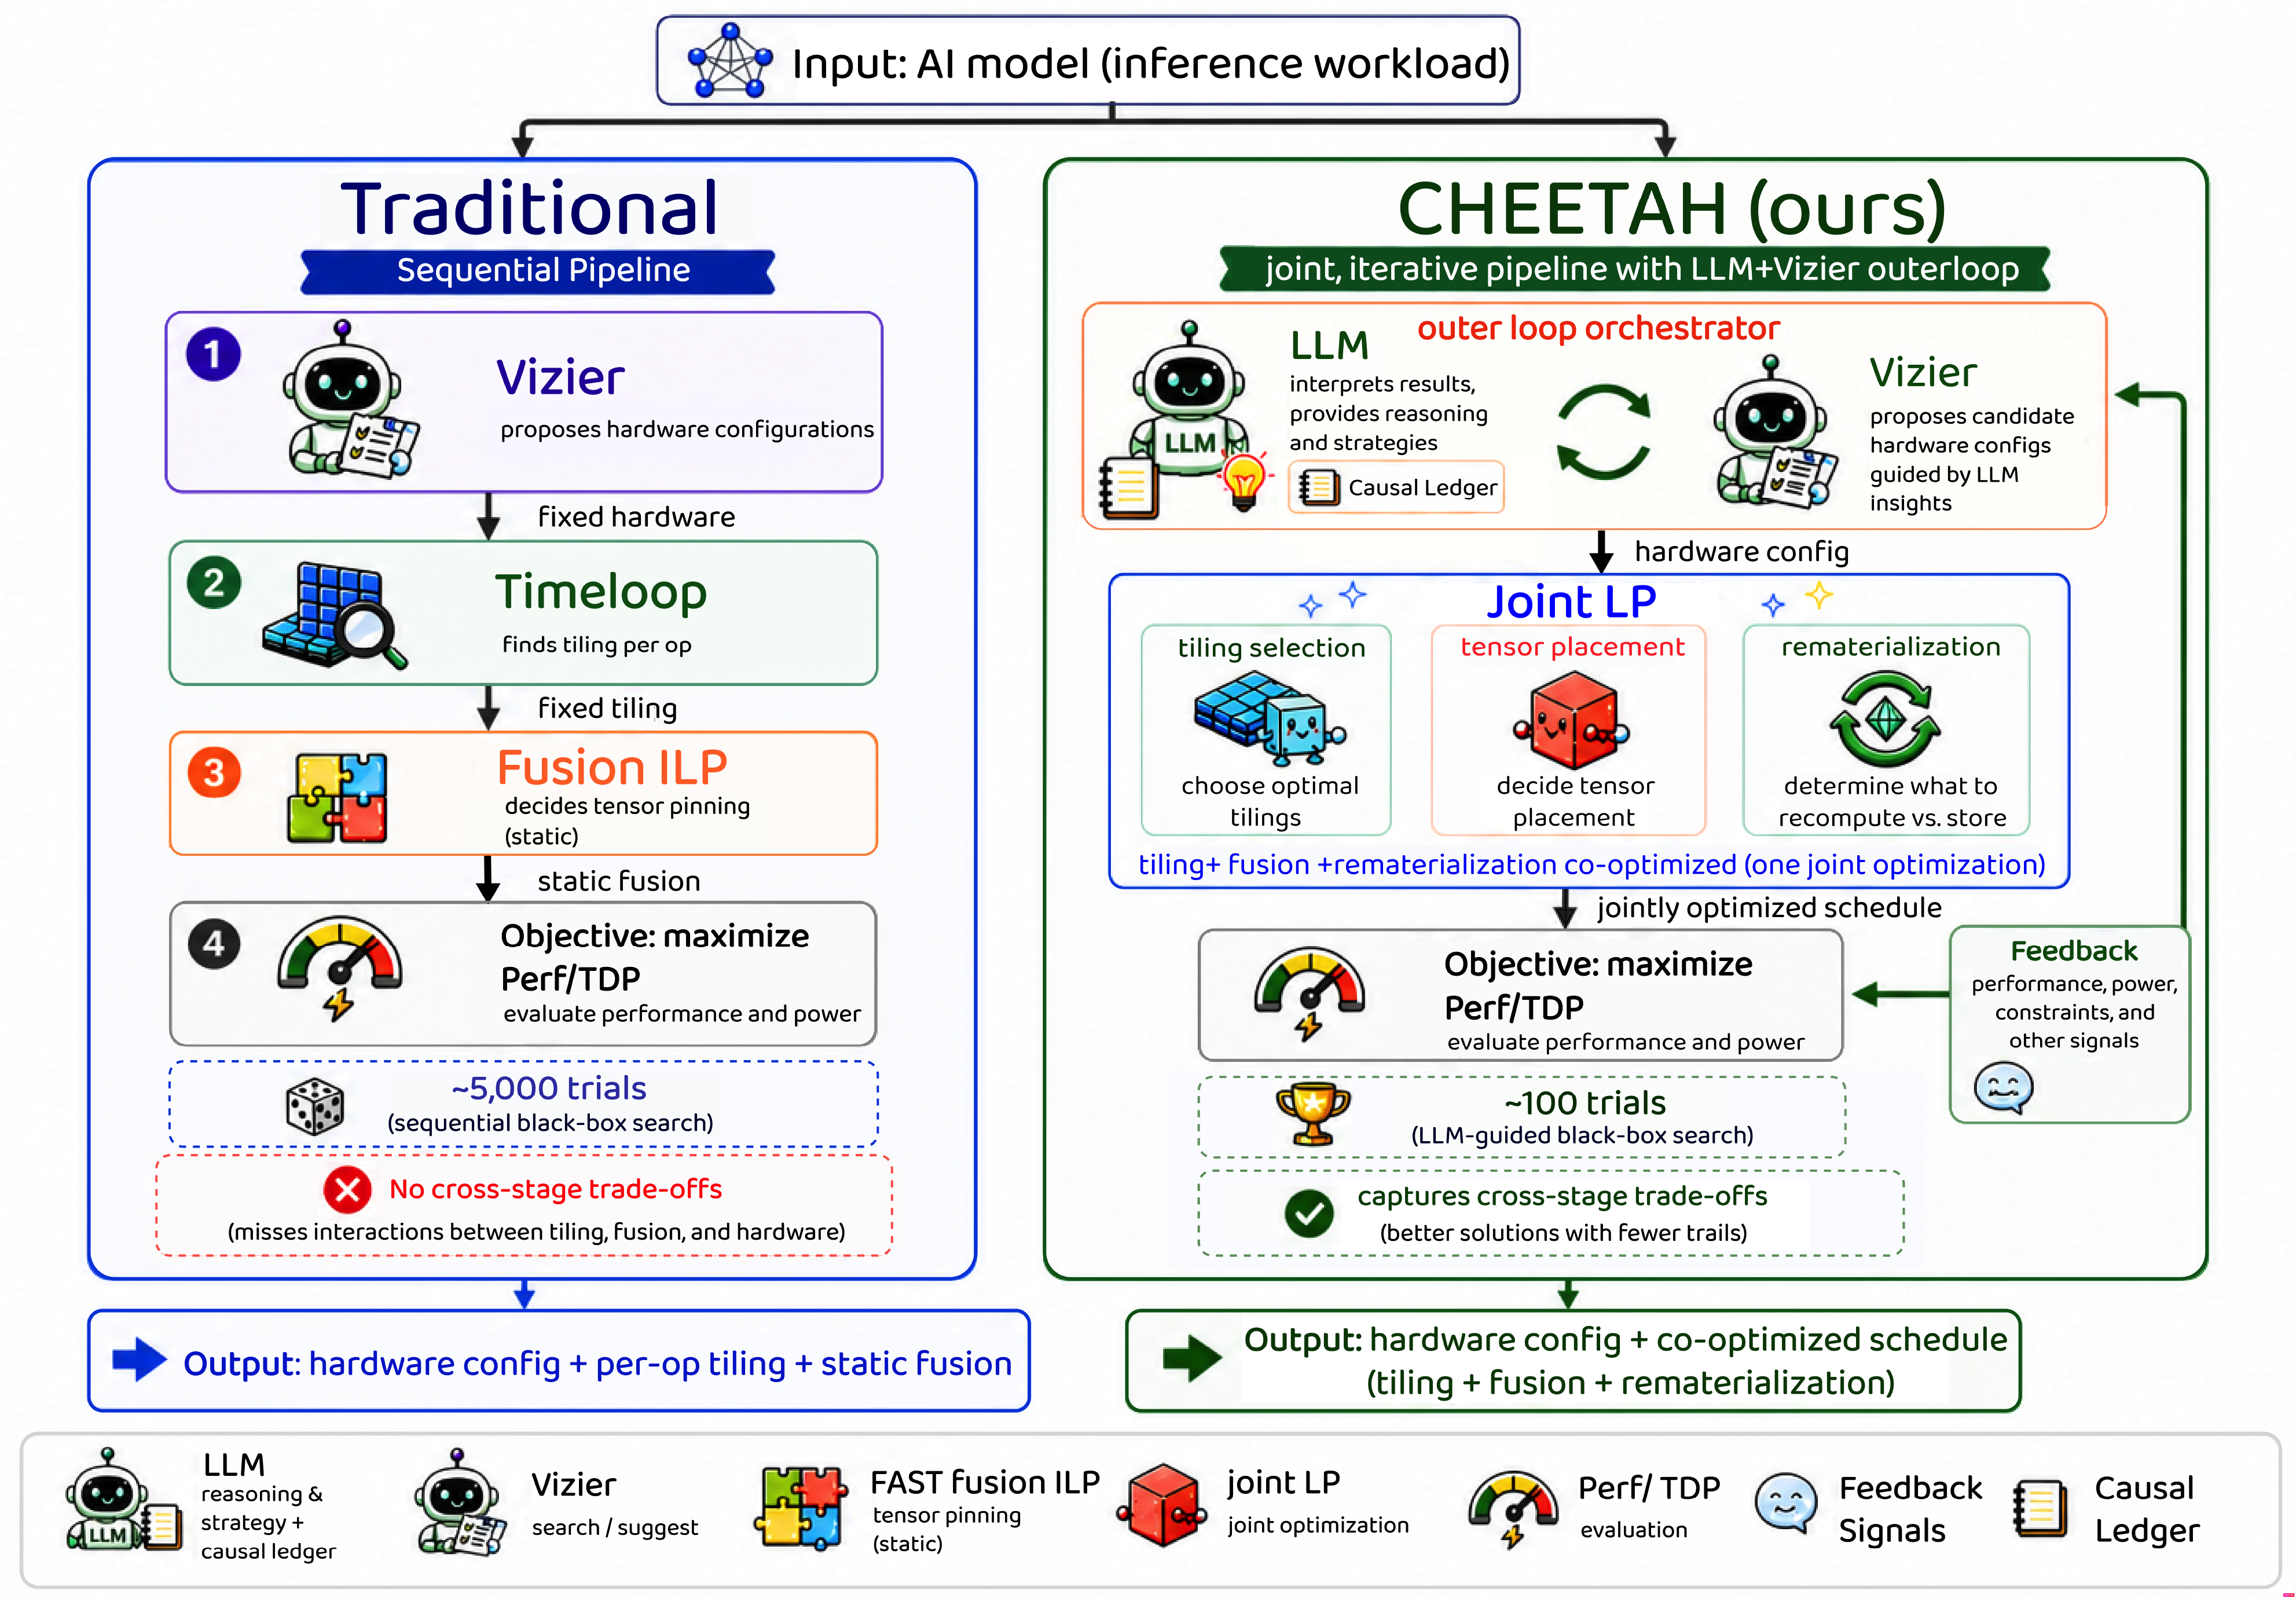
\includegraphics[width=1.0\linewidth]{figs/cheetah_v4_new.png}
    % \caption{\textbf{FAST vs.\ FAST-CORGI pipeline comparison.} 
\caption{Sequential vs Our Unified Optimization Paradigm.
(Left) Baseline methods decouple hardware search, operation-level tiling, and static fusion; precluding cross-stage trade-offs.
(Right) CHEETAH presents a unified LLM-driven LP-solver-based framework that jointly optimizes tiling, placement, and rematerialization while learning from a causal ledger.}
\label{fig::workflow}
\end{figure}
% The rapid evolution of deep learning workloads varies from convolutions to self-attention (LLaMA), mixture-of-experts (DeepSeek-V3), and state-space models (Mamba). These diverse architectures serve billions of daily users, and have fundamentally shifted the requirements for hardware acceleration. As foundation models continue to scale in parameters, the primary cost and bottleneck of model deployment has shifted from training to inference. Therefore much recent research has been focused on optimizing for more efficient execution and throughput across diverse, high-dimensional workloads. General-purpose GPUs remain largely designed for graphics-heavy throughput, and leave substantial efficiency and compute on the table at these tasks. Therefore we are motivated to design targeted accelerators that are optimized for handling the varying tensor shapes and data-reuse patterns of modern deep learning architectures.
% Much research has been done in accelerating inference through custom accelerator design, more efficient neural network (NN) batching algorithms, and domain specific packages and languages that aim to speed up general NN inference. For example, the widely adopted Flash Attention uses tiling to provide significant speedups by optimizing memory movement between SRAM and DRAM. Co-design takes this a step further by aiming to optimize hardware, software and scheduling to unlock performance neither could reach independently. The traditional framework of doing this is a sequential pipeline of heuristics tools, requiring human engineers to iterate through a large search space for months from testing for the size of DRAM, to determining higher level scheduling problems. Optimizing each piece of this complex pipeline is extremely challenging, since hardware datapaths, software schedules, and compiler transforms across a combinatorial space exceeding $\mathcal O(10^{2300})$.
The AI inference demand is expected to grow by $10,000\times$ over the next 5 years \citep{cra2026aifuture}. General-purpose accelerators leave significant efficiency gains unrealized, which motivates the design of targeted custom accelerators. Co-design, which jointly optimizes hardware-software (HW/SW), and scheduling for target workloads, offers a path to unlock performance efficiency for the upcoming inference era. However, the prevailing approach relies on sequential pipelines of heuristic tools, a slow, human-driven process navigating a combinatorial search space exceeding $\mathcal O(10^{2300})$ \citep{zhang_fast}. State-of-the-art frameworks like FAST \citep{zhang_fast} improve on this through an automated flow (a hardware proposer feeds an operation-level tiling agent, which feeds a downstream fusion solver), but remain fundamentally decoupled: a tiling that slightly reduces compute efficiency may shrink the working set enough to eliminate a DRAM bottleneck, yet sequential pipelines cannot discover such cross-stage trade-offs.

% The co-design problem is increasingly important as inference efficiency is the dominant AI workload and is rapidly growing. Therefore industry leaders such as NVIDIA and Google have designed chips for improved hardware-native agentic AI and , and state-of-the-art frameworks such as FAST, address this through a sequential decomposition of heuristics (a hardware proposer feeds an operation-level tiling agent, which feeds a downstream fusion solver). While FAST-generated accelerators can provide increased speedups over baseline TPU-v3, this decoupled approach is limited since it cannot capture cross-stage trade-offs. A tiling configuration that is \textit{locally} optimal for one layer may create an activation footprint that later prevents \textit{global} fusion, while a slightly slower tiling might shrink the working set enough to eliminate a DRAM bottleneck entirely. Sequential pipelines are systematically unable to express these interactions, leading to locally good but globally sub-optimal designs. 
Unifying the design space into a single convex relaxation yields previously infeasible global optima. Specifically, we introduce CHEETAH: a custom inference accelerator design framework that unlocks globally optimized designs with a dual-loop. Our inner-loop is a novel large-scale Linear Program (LP) to precisely mathematically model strict design decisions and constraints that must not be violated. The LP captures trade-offs for targeted workloads through time-indexed placement and rematerialization, thus allowing tensors to be dynamically pinned, evicted, recomputed across inference timesteps. We further extend our reformulation to internalize tiling selection into the LP, by introducing Pareto-pruned tiling variables and the McCormick linearization (a convex relaxation used for optimization of bilinear problems \citep{mccormick1976computability}). By exploiting the structural invariance of our matrices across hardware trials, we also adapt a GPU-accelerated primal-dual solver in JAX \citep{jax2018github} that can resolve millions of variables to rapidly reduce trial time from days to hours. This allows the LP solver to jointly reason about hardware configuration, activation placement, and weight pinning in a single pass, while providing feedback signal via Lagrangian duals.

\paragraph{One program, many architectures.} A natural question is how a single program can co-design accelerators for workloads as different as EfficientNet, the Llama family, DeepSeek-V3's mixture-of-experts, and the Stable Diffusion UNet. The LP is \emph{not} per-architecture: it is defined over a generic graph intermediate representation, a directed acyclic graph of operations, each carrying a Timeloop-derived tile-configuration Pareto set and a roofline, connected by edges with residency. A depthwise convolution, a dense GEMM, an attention matmul, and an expert feed-forward are all simply ``operations with shapes''; the architecture-specific content lives entirely in the coefficients (operation shapes, Pareto data, and edge topology), never in the structure of the program. Architecture-specific decisions (a KV-cache budget, mixture-of-experts expert-residency, diffusion cross-step reuse) are optional constraint families that switch on only when the relevant operation type is present and are inert otherwise. One program therefore covers every architecture the way a single register allocator compiles every source language: it operates on the graph, not the workload.

Our outer-loop framework stacks a black-box optimizer (Google Vizier \citep{google_vizier}) to propose candidate hardware configurations defined by a set of hyperparameters (e.g., processing element grid dimensions, systolic array sizes, DRAM size, etc), while a LLM is used for efficient search-space steering. The LLM acts as a causal architect, interpreting a compact trial ledger of roofline checks and LP feedback diagnostics to propose constrained architectural search input for Vizier. This prevents the search-space gaming typical of black-box optimizers in wide design regions, and reduces the need for thousands of sequential trials via Bayesian search strategies in Vizier to learn good vs bad neighborhoods in search topology. Our results demonstrate that the LLM Architect framework further reduces invalid hardware trials from 24.5\% under vanilla Vizier to 5.9\%, to reach the Pareto frontier faster than the next strongest baseline. We validate all results with Model Flop Utilization (MFU) and roofline lower-bound audits, ensuring predicted latencies are physically grounded in compute and memory throughput limits. Figure~\ref{fig::workflow} outlines the comparative difference between the standard sequential workflow and our joint optimization paradigm. 
% \todo{Add best of both worlds, strengths from principled LP side, from LLM aggregate info side}
% \todo{Aggregates past experience to gain insight into steering hardware-software co-design. We offload the strict solves, with constraints that must the strictly respected, to the LP solve part. This combines the best of both worlds.} 
\paragraph{Contributions.} We reformulate the fundamental HW/SW co-design problem into a unified  framework in CHEETAH, combining principled mathematical rigor of the LP formulation to solve strict design decisions optimally, with the powerful aggregation and causal learning of an LLM Architect outer loop for meta-optimization. Our open-source repository for full reproducibility is at \href{https://anonymous.4open.science/r/CHEETAH-B268/readme}{https://anonymous.4open.science/r/CHEETAH-B268/}.

\begin{enumerate}
    \item \textbf{CHEETAH-V0 - Dynamic Placement with Rematerialization:}
    We introduce time-indexed LP variables $p_{i,t}^k$ and rematerialization variables $r_{i,t}$ to enable cheap recompute operations instead of paying DRAM reload costs, supporting skip connections and multi-fanout nodes.

    \item \textbf{CHEETAH-V1 and V3 - Joint Tiling-Fusion via Classical Convex Modeling:}
    We unify tiling and fusion into a single LP problem by introducing tiling selection variables $y_{i,c}$, and employ \textbf{McCormick envelopes} to exactly linearize the bilinear interaction between tiling and tensor pinning; V3 then promotes the chip's MAC count and bandwidth to decisions and replaces the aggregate roofline with a \textbf{disaggregated perspective epigraph} that is the exact convex hull of the per-tile roofline disjunction. Both are classical tools of mathematical programming (McCormick's 1976 envelopes and epigraph/perspective reformulation) that the accelerator co-design literature does not use, because its pipelines are built from simulators and heuristics rather than from programs. Applied here they buy two things at once: a parameter-free relaxation that is exact at every integer vertex, so the LP is simultaneously an optimizer and a valid lower bound, and a coupling that internalizes the tiling-placement trade-off to discover design points that sequential pipelines systematically miss.
    % This enables the LP to discover trade-offs where accepting a suboptimal tiling configuration enables superior fusion, or vice versa---precisely the cross-stage interactions that the sequential pipeline cannot capture.
    \item \textbf{VM-One-Armed-Rescue Solver:} The McCormick linearization that makes V1 exact also \emph{blows up} the constraint matrix (for DeepSeek-V3, ${\sim}2.5$M variables, ${\sim}3.0$M constraints, and ${\sim}6.1$M nonzeros) and leaves it severely ill-conditioned, with coefficients spanning ${\sim}10$ orders of magnitude. Stock first-order GPU solvers (cuPDLP) and CPU simplex/barrier (HiGHS) stall or diverge, with the primal or dual side lagging. We introduce \textbf{VM-One-Armed-Rescue}, a matrix-free JAX solver that augments restarted PDHG with a diagonal \emph{variable-metric} rescaling and a one-sided ``rescue'' restart, resolving these LPs to dual convergence in seconds. To our knowledge it is the first solver to make the McCormick-linearized joint tiling--fusion--placement co-design LP tractable at LLM scale: the enabling step that collapses a days-long search into hours (Section~\ref{sec:solver_vm}).

    \item \textbf{LLM-guided Causal Architect:} The LLM outer loop steers hardware search by interpreting \emph{converged Lagrangian dual signals} from the inner LP together with a Causal Ledger of past trials to perform targeted subspace interventions, transforming black-box search into a structured, diagnostic-driven process. To our knowledge, CHEETAH is the \textbf{first} to steer an LLM-guided architecture search with the converged Lagrangian dual variables of a co-design LP: the duals \emph{indicate} where to search while the LP retains every optimality certificate; the LLM proposes, the solver never loses rigor. The Architect guides Vizier through widened search spaces, reducing invalid trials by ${\sim}4\times$ ($24.5\%\!\to\!5.9\%$) while preserving the global optimal score, and enables profile-specific designs (speech models may emphasize latency, while data-synthesis models may prioritize bandwidth).
    \item \textbf{Certificates, not counters:} Every CHEETAH schedule ships with an LP optimality certificate: the converged dual bound against which the realized schedule is measured, with the relaxation gap reported per workload and the integral optimum certified exactly on chain-structured models. A cycle-accurate RTL replay then confirms, decision by decision (tile choice, residency, eviction, rematerialization), that the plan executed as planned with byte-exact memory occupancy. This is a stronger guarantee than the ``did the optimization fire'' checks that agentic kernel optimizers use to validate hardware-aware code~\citep{tschand2026hawkeye}: a counter confirms a feature was used, a certificate bounds how far the result can be from optimal.

    \item \textbf{Speedup:} Our method demonstrates an average speedup of $\sim22.07\times$ over the baseline across a wide range of $12$ workloads ($11$ vision and language models plus the Stable Diffusion~1.5 UNet), reaching up to ${\sim}40.1\times$ on a single workload, as shown in Figure~\ref{fig:speedup} below. \todo{averages and Figure~\ref{fig:speedup} to be refreshed once SD1.5-UNet is added to the search plots}

    % profiles into consideration to push the black-box optimizer responsible for hardware suggestions to output with structured reasoning about architectural trade-offs. 

\end{enumerate}

\begin{figure}[ht!]
    \centering
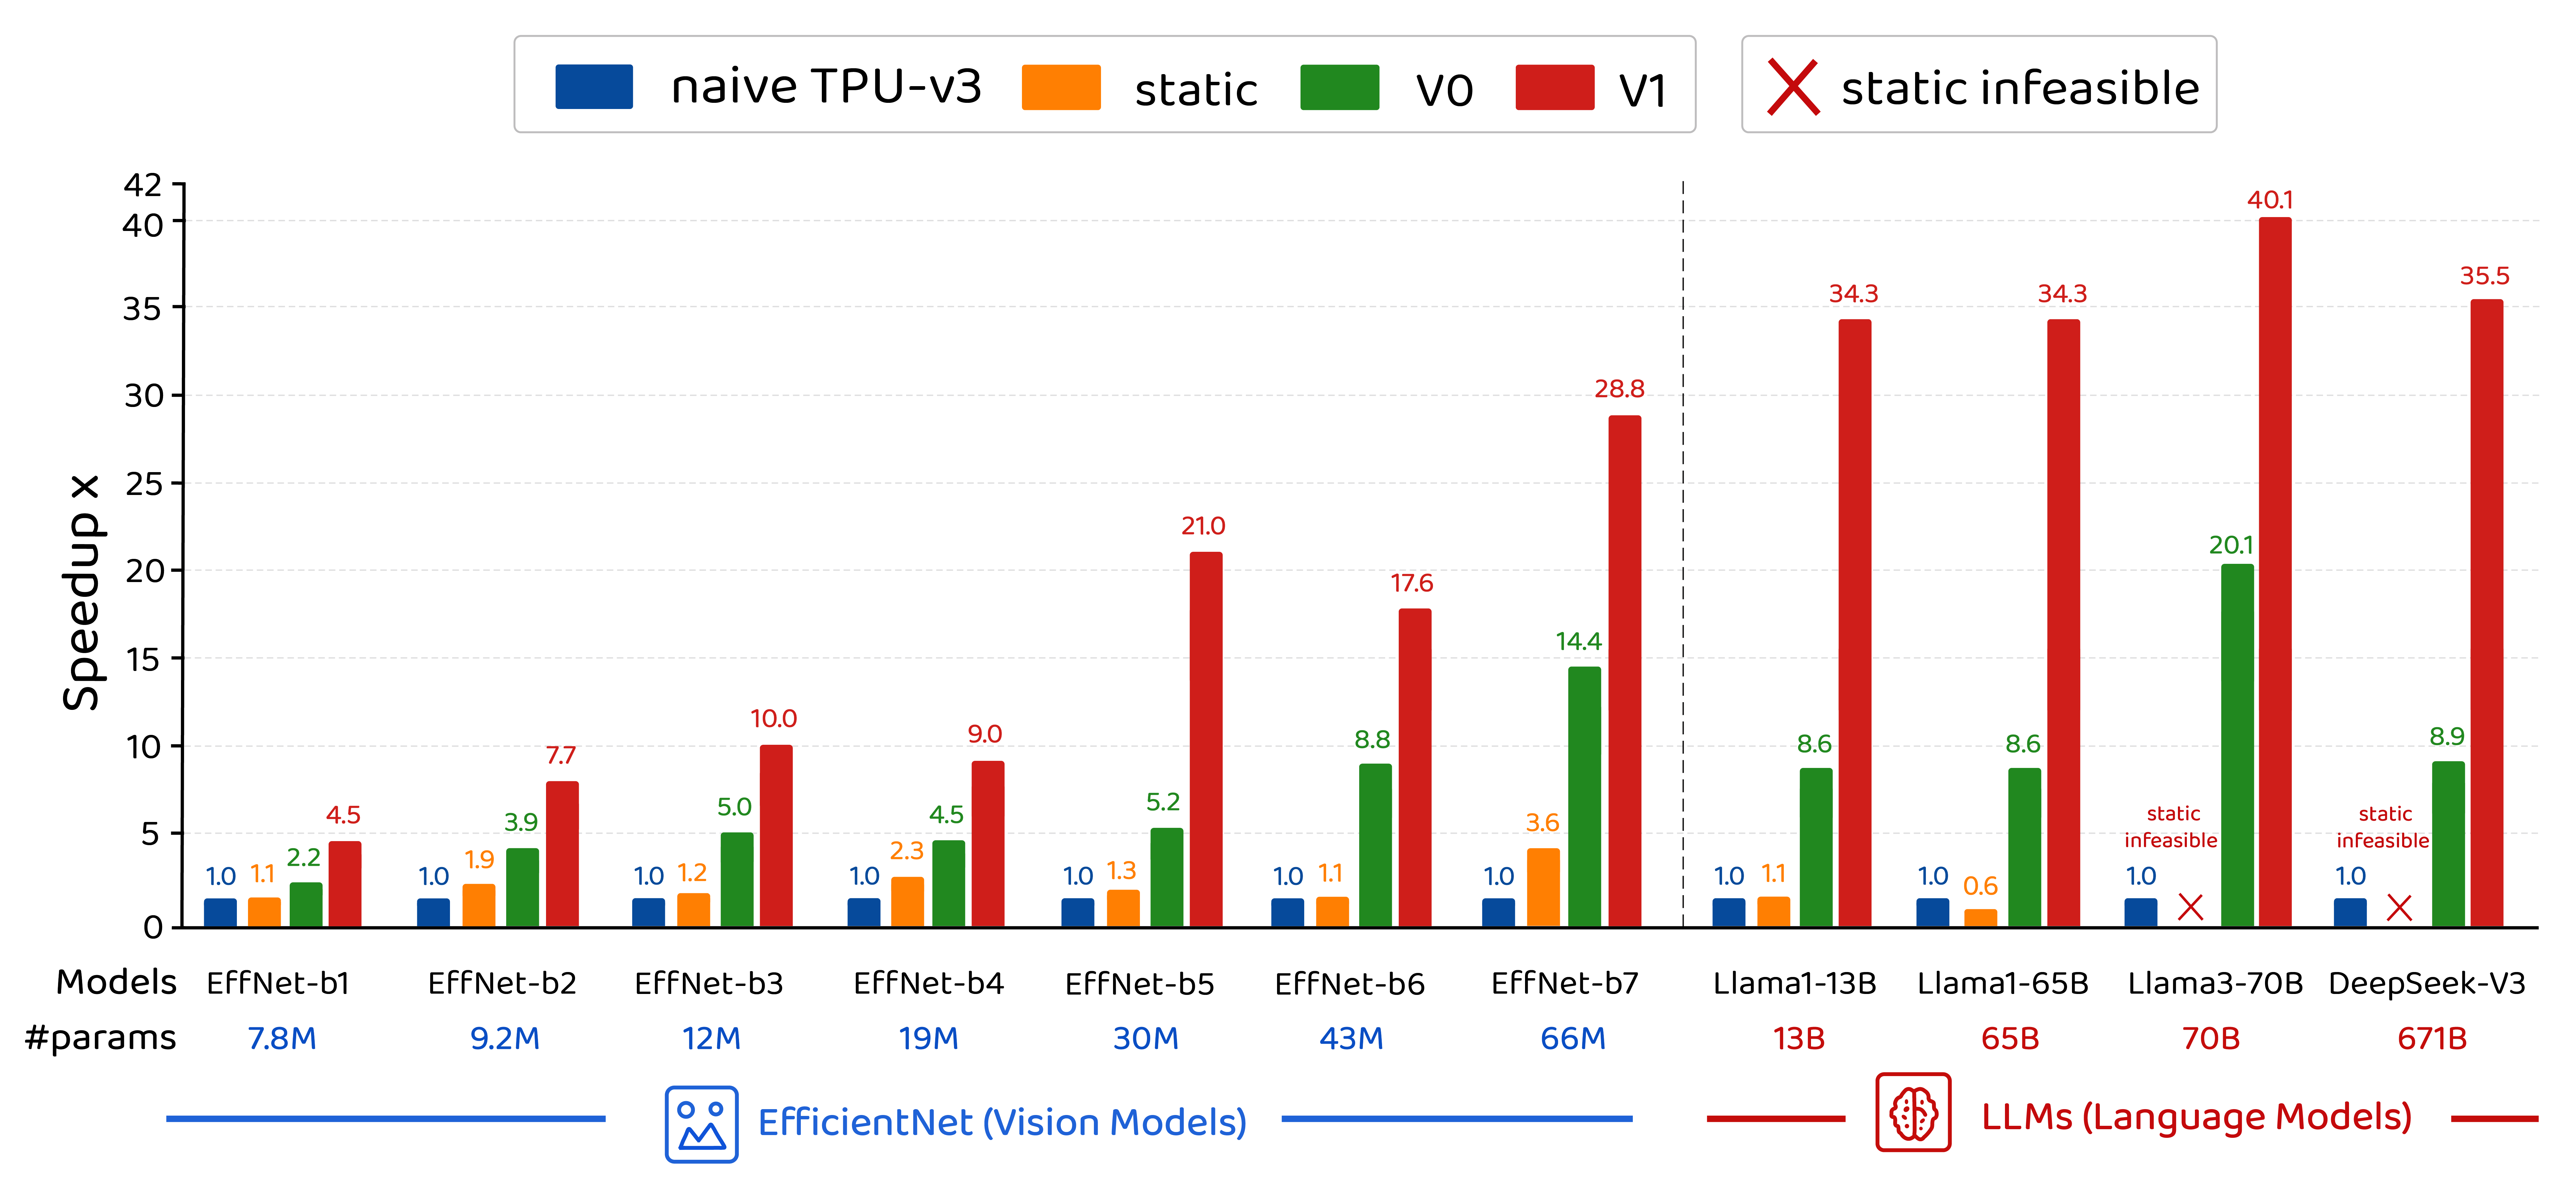
\includegraphics[width=1.0\linewidth]{fig3/speedup_final_v3.png}
\caption{Speedup over modeled TPU-v3 baseline for each workload and formulation: CHEETAH-V1's joint tiling-fusion optimization achieves up to $\sim$40.1$\times$ acceleration, while static fusion is infeasible on large-scale LLMs. Progressive gains are visible across formulations: V0's dynamic placement improves over static by $2$--$20\times$, while V1's joint tiling-fusion adds another $2$--$4\times$ on top. See Section~\ref{sec:experiments} for full analysis and wall-clock time breakdowns.}
\label{fig:speedup}
\end{figure}

CHEETAH reframes accelerator co-design from a sequential pipeline of heuristics into a single certified optimization. Its inner LP provably \emph{contains} the map-then-fuse pipelines of prior work (Theorem~\ref{thm:containment}) and returns a certified lower bound on schedule quality, so the field's usual ``$N\times$ over a baseline'' becomes ``within a certified gap of the optimum''; its outer loop couples this rigor with an LLM that reads the LP's own Lagrangian duals to steer the hardware search. The consequences are concrete: a ${\sim}22\times$ average (up to ${\sim}40\times$) speedup over a modeled TPU-v3 across $12$ vision, language, and diffusion workloads, every design validated by cycle-accurate RTL, six physical-feasibility gates, and roofline lower-bound audits, and a co-design loop that runs in \emph{hours} rather than months. The human's role shifts accordingly: they write constraints (area, power, capacity, and the cost model), not designs, and a new chip or a new workload enters the same program as new columns and rows rather than as a new search. We view this as a step-change in \emph{how} accelerators are designed: not a faster point inside an existing search, but a reformulation that makes the global optimum (and a proof of how close a design sits to it) attainable for the inference era.

\paragraph{Beyond prefill: shrinking the decode memory wall.} The speedups above are largest in the compute-bound \emph{prefill} phase, where scheduling has the most room. Realistic LLM \emph{serving}, however, is dominated by autoregressive \emph{decode}, where generating each token reloads the full weights and a growing KV cache from DRAM: the bottleneck shifts from compute to memory, and on fixed hardware no schedule can move it because the bytes are schedule-invariant. CHEETAH's co-design attacks this wall directly and jointly, by \emph{sizing on-chip global memory against a bounded, quantized KV cache} so that the cache is co-designed to fit on chip and its per-token read never touches DRAM. \todo{STALE FRAMING: our own newer results (\cref{sec:batch_sensitivity}, App.~N, Limitations) show the decode wall is MoE WEIGHT RELOAD (${\sim}98\%$ of decode traffic) with KV negligible. Rewrite this and the matching abstract clause around the sparse-routing/speculation story already written below.}The structural insight the program exploits is that on-chip memory should hold the KV cache, not the weights: model weights ($13$--$70$\,GB) cannot fit and must stream, but the KV cache can be bounded by eviction and shrunk by quantization until it fits, and it is re-read every decode step, so every byte of on-chip memory spent on it pays off once per generated token. Sizing the global buffer, the eviction budget, and the KV precision in one program is what shrinks the decode memory wall.

\paragraph{Why the decode wall does not dissolve under load: sparse routing defeats batching.}
For a dense model the decode memory wall is, in principle, a low-batch problem:
a larger serving batch amortizes each weight load perfectly, because the same
weights serve every token in the batch, so at high enough throughput the wall
recedes on its own. A sparse mixture of experts breaks this argument, and this
is what makes the co-design necessary rather than merely convenient. Under
top-$k$ routing the set of experts a decode step must load is the \emph{union}
of the experts its tokens select, so a larger batch touches \emph{more} experts:
the expected number of distinct experts follows $n(1-(1-k/n)^{B})$, which for
DeepSeek-V3 ($n=256$, $k=8$) rises from $8$ experts at $B=1$ to $163$ at
$B=32$ and $252$ at $B=128$. The reload therefore \emph{grows} with batch,
from $19$ to $598$~GB per step across that range, and although the per-token
cost does fall, it falls only from $19$ to $4.7$~GB, a $4\times$ amortization
bought with a $128\times$ increase in batch, and it saturates once essentially
every expert is swept. The wall is thus a structural property of sparse serving
rather than an artifact of small batches, and we confirm the consequence
empirically in \cref{sec:batch_sensitivity}: the speculative width the program
selects rises rather than collapses as batch grows, doubling with every
fourfold increase in batch, and the certified serving advantage rises
monotonically from $33.1\times$ at $B=1$ to $48.6\times$ at $B=128$. Two
mechanisms that are usually described as competing amortizers, batching and
speculation, are complementary here, precisely because batching amortizes so
poorly under sparse routing.

We present the work as a progression, so that each formulation's contribution can be read on its own terms. Section~\ref{sec:related} positions CHEETAH against prior mapping, co-design, and compilation systems (Table~\ref{tab:capability-matrix}). Section~\ref{sec:methods} builds the formulation in rungs: CHEETAH-V0 (Section~\ref{sec:v0}) adds time-indexed placement and rematerialization to the static fusion ILP; V1 (Section~\ref{sec:v1}) brings tiling inside the program, using Pareto pruning to compress the raw tile space and McCormick envelopes to flatten the resulting bilinear coupling into a linear program; V2 adds memory sizing and tile-dependent residency; and V3 (Section~\ref{sec:v1}) promotes the hardware itself to a decision under a disaggregated perspective epigraph, with the solver (Section~\ref{sec:solver_vm}) and the LLM-guided outer loop closing the loop. Section~\ref{sec:experiments} reports the progressive gains across these rungs together with the same-silicon fixed-hardware study, each result grounded by roofline, MFU, and manufacturability validators; Section~\ref{sec:rtl_validation} replays the schedules on cycle-accurate RTL; Section~\ref{sec:tco} reads the outcome in FAST's own cost model; and the appendices carry the containment theory, the solver, and the deficit and sensitivity analyses.

% In addition to efficiently enabling more globally optimized accelerator designs, we anticipate that future work may build off this foundation to implement custom Flash Attention type speedup mechanisms for individual hardware (such as RTX5090) and workloads (such as LLama70B) tractably within hours, as well as quickly and efficiently design custom accelerators for targeted inference tasks. 
% compromise on any single workload; a growing body of evidence suggests that workload-specialized designs can deliver $2$--$6\times$ improvements in performance per watt.
% The resulting system replaces FAST's sequential Timeloop$\rightarrow$fusion~ILP pipeline with a single LP that jointly optimizes tiling, fusion, and memory scheduling, while preserving Vizier's outer loop over hardware configurations (or replacing it with LLM-guided search).

% Furthermore, FAST's fusion ILP uses static tensor placement: a tensor is either pinned for the entire inference pass or not at all.
% This is overly conservative for models with long dependency chains or skip connections, where different tensors are live at different times during execution.
% A dynamic placement strategy that can evict and re-pin tensors across timesteps could substantially improve global memory utilization. Joint Optimization is the only way to solve the "Memory Wall" for large scale models like DeepSeek-V3.

% FAST operates via a three-stage sequential pipeline (Figure \ref{fig::workflow}): (1)~a black-box optimizer (Google Vizier \citep{google_vizier}) proposes a hardware configuration defined by 16 hyperparameters---PE grid dimensions, systolic array sizes, buffer capacities, DRAM channels, and batch size; (2)~a scheduling engine (Timeloop \citep{timeloop}) finds the best tiling and mapping for each operation independently given the fixed hardware; and (3)~an integer linear program (ILP) decides which tensors to pin in the on-chip Global Memory to reduce DRAM traffic.
% The result of each trial---predicted performance per TDP---is fed back to Vizier, which proposes the next hardware configuration, repeating for thousands of trials until convergence.


% automate the framework with SkyDiscover Loop for profile and context aware co-design. Therefore in less than five hours, we are able to find an more performant design spec than the strongest baseline on designing , in terms of both perf/TDP and speedup. Our experiments also include freezing any hardware at input, and reducing the scheduling, tiling, etc search to just the LP can yield speedups of avg 2.2x than just the base hardware along. We anticipate that future work may build off this foundation to implement custom Flash Attention type speedup mechanisms for individual hardware (such as RTX5090) and workloads (such as LLama70B) tractably within hours. 

% Our propose the formulation for global co-design for a custom accelerator as a large scale linear program which captures strict dependencies and tradeoffs sequential methods may miss. Our LP formulation captures scheduling, tiling, rematerialization, and is able to solve matrices at scales of $6{,}319 \times 4{,}516$,\ nnz$=829{,}852$ \& $3{,}669{,}793 \times 3{,}263{,}443$,\ nnz$=7{,}342{,}293$ \& $2{,}983{,}450 \times 2{,}504{,}019$,\ nnz$=6{,}094{,}156$ quickly, by utilizing a JAX based large scale solver. Our insight is that despite the challenging large scale of the problem, the structure of the matrices, once formed, retain the same structure. Therefore we are able to design one preconditioning scheme to these large scale systems matrices that can be re-used across any NN. This also allows us to capture dependencies prior methods cannot, for example our formulation introduces a dynamic placement strategy that can evict and re-pin tensors across timesteps could substantially improve global memory utilization. Joint Optimization is the only way to solve the "Memory Wall" for large scale models like DeepSeek-V3. 

% For EfficientNet-B7 at $L=400$ operations and $T=400$ timesteps, the V1 LP contains approximately $2$ million variables and $5$ million constraints with $15$--$25$ million nonzeros. To better solve such large-scale LP problems more efficiently, we implement our own variant of a GPU-accelerated solver based on recent primal-dual LP algorithm \citep{applegate2022practicallargescalelinearprogramming}. We extend its original formulation in various ways and benchmark our implementation compared to existing commercial SciPy solvers, which showcase the advantage of our solver. To keep the main context clean and focused, we defer LP solver-related details to Appendix \ref{app:solver}.

% A large number of black box optimization tools to handle this large search space have been recently proposed, such as Google's Vizier, Meta's AX, and Optuna. In addition search strategies are also explored, for example Google's Vizier proposes numerous methods Gaussian Process Upper Confidence Bound, Eagle Strategy as a metaheuristic optimization algorithm designed for global optimization via a two-stage hybrid approach that combines global exploration with intensive local search, and Linear Combination Swarm (LCS). However these methods share certain limitations, since they cannot globally capture the tradeoffs and tensions between sequential decisions and rely on brute force iterations. This requires human engineers to spend months of compute and thousands of repetitive trials to get improvements, without feedback on what might be globally optimal. 

% While this sequential decomposition makes the problem tractable, it introduces a fundamental limitation: \emph{each stage takes the previous stage's output as fixed input, preventing the discovery of solutions that require trading off across stages.} Consider a concrete example: for a depthwise-separable convolution layer in a NN, a search tool such as Timeloop might select a tiling configuration that maximizes compute utilization at $74\%$, producing an activation working set of $6$ MiB. THe stacked The downstream fusion ILP solver tool receives this fixed working set size, cannot fit the tensor into the $128$ MiB Global Memory alongside other pinned tensors. However, an alternative tiling configuration with slightly lower utilization ($70\%$) might produce a working set of only $3$ MiB, enabling the fusion solver to pin an additional weight tensor that eliminates a DRAM bottleneck entirely, thus yielding a net $>20\%$ cycle reduction despite the $4\%$ utilization loss. Therefore these sequential pipelines systematically misses such cross-stage trade-offs.

% The rapid evolution of deep learning workloads has created a compelling opportunity for domain-optimized inference accelerators.
% Production models now serve billions of daily users, and the computational demands of architectures based on depthwise-separable convolutions (EfficientNet), self-attention (BERT, LLaMA), mixture-of-experts (DeepSeek-V3, Mixtral), and state-space models (Mamba) differ dramatically in their compute-to-memory ratios, tensor shapes, and data reuse patterns. However although the NN training strategy has been scaled up and we've done a lot of work on it, we now face the inference bottle neck era since general-purpose hardware, Nvidia's gaming GPUs are not necessarily optimized for deep learning tasks, and leaves a huge amount of compute on the table.